% BU ECE template for MS thesis and PhD dissertation.
%
%==========================================================================%
% MAIN PREAMBLE 
%==========================================================================%
\documentclass[12pt,letterpaper]{report}          % Single-sided printing for the library
%\documentclass[12pt,twoside]{report} % Double-sided printing
\usepackage[intlimits]{amsmath}
\usepackage{amsfonts,amssymb}
\DeclareSymbolFontAlphabet{\mathbb}{AMSb}
%\usepackage{natbib}
\usepackage{apalike}
\usepackage{float}
\usepackage[bf]{caption}       
\setcaptionmargin{0.5in}
\usepackage{fancyhdr}
%\usepackage{fancyheadings}
\usepackage{fancybox}
\usepackage{ifthen}
\usepackage{bu_ece_thesis}
\usepackage{url}
\usepackage{lscape,afterpage}
\usepackage{xspace}
\usepackage{epstopdf} 
\usepackage{subfig}
\usepackage{bm}

%==========================================================================%
%%% graphicx and pdf creation
\usepackage{graphicx}
\usepackage{appendix}
%\usepackage{psfrag}
%\DeclareGraphicsExtensions{.eps}   % extension for included graphics
%\usepackage{thumbpdf}              % thumbnails for ps2pdf
%\usepackage[ps2pdf,                % hyper-references for ps2pdf
%bookmarks=true,%                   % generate bookmarks ...
%bookmarksnumbered=true,%           % ... with numbers
%hypertexnames=false,%              % needed for correct links to figures !!!
%breaklinks=true,%                  % breaks lines, but links are very small
%linkbordercolor={0 0 1},%          % blue frames around links
%pdfborder={0 0 112.0}]{hyperref}%  % border-width of frames 
%                                   % will be multiplied with 0.009 by ps2pdf
%\hypersetup{
%  pdfauthor   = {Joe Graduate <joe.graduate@bu.edu>},
%  pdftitle    = {dissertation.pdf},
%  pdfsubject  = {doctoral dissertations},
%  pdfkeywords = {mathematics, science, technology},
%  pdfcreator  = {LaTeX with hyperref package},
%  pdfproducer = {dvips + ps2pdf}
%}
%==========================================================================%
% customized commands can be placed here
%\newcommand{\figref}[1]{Figure~\ref{#1}}
%\newcommand{\chapref}[1]{Chapter~\ref{#1}}
%\newcommand{\latex}{\LaTeX\xspace}
%==========================================================================%

%==========================================================================%
% BEGIN
%==========================================================================%

%% REMOVE THIS COMMAND AFTER EDITS ARE DONE
%% mark PJE comments in the text
\newcommand{\jcom}[2]{\marginpar{{\footnotesize \bf #1}}{\it {#2}}}
\begin{document}

% The preliminary pages
% This file contains all the necessary setup and commands to create
% the preliminary pages according to the buthesis.sty option.

\title{Space-time Sampling Strategies for Electronically Steerable Incoherent Scatter Radar}

\author{John Swoboda}

% Type of document prepared for this degree:
%   1 = Master of Science thesis,
%   2 = Doctor of Philosophy dissertation.
%   3 = Master of Science thesis and Doctor of Philosophy dissertation.
\degree=2

\prevdegrees{B.S., Rensselaer Polytechnic Institute, 2007  \\ M.S., Rensselaer Polytechnic Institute, 2008} 


\department{Department of Electrical and Computer Engineering}

% Degree year is the year the diploma is expected, and defense year is
% the year the dissertation is written up and defended. Often, these
% will be the same, except for January graduation, when your defense
% will be in the fall of year X, and your graduation will be in
% January of year X+1
\defenseyear{2016}
\degreeyear{2017}

% For each reader, specify appropriate label {First, Second, Third},
% then name, and title. IMPORTANT: The title should be:
%   "Professor of Electrical and Computer Engineering",
% or similar, but it MUST NOT be:
%   Professor, Department of Electrical and Computer Engineering"
% or you will be asked to reprint and get new signatures.
% Warning: If you have more than five readers you are out of luck,
% because it will overflow to a new page. You may try to put part of
% the title in with the name.
\reader{First}{Joshua L. Semeter, PhD}{Professor of Electrical and Computer Engineering}
\reader{Second}{David A. Castañón, PhD}{Professor of Electrical and Computer Engineering\\Professor of Systems Engineering}
\reader{Third}{S. Hamid Nawab, PhD}{Professor of Electrical and Computer Engineering\\Professor of Biomedical Engineering}
\reader{Fourth}{Philip J. Erickson, PhD}{Assistant Director, MIT Haystack Observatory}

% The Major Professor is the same as the first reader, but must be
% specified again for the abstract page. Up to 4 Major Professors
% (advisors) can be defined. 
\numadvisors=1
\majorprof{Joshua L. Semeter, PhD}{\mbox{Professor of Electrical and Computer Engineering}}
%\majorprofb{First M. Last, PhD}{{Professor of computer Science}}
%\majorprofc{First M. Last, PhD}{{Professor of Astronomy}}
%\majorprofd{First M. Last, PhD}{{Professor of Biomedical Engineering}}

%%%%%%%%%%%%%%%%%%%%%%%%%%%%%%%%%%%%%%%%%%%%%%%%%%%%%%%%%%%%%%%%  

%                       PRELIMINARY PAGES
% According to the BU guide the preliminary pages consist of:
% title, copyright (optional), approval,  acknowledgments (opt.),
% abstract, preface (opt.), Table of contents, List of tables (if
% any), List of illustrations (if any). The \tableofcontents,
% \listoffigures, and \listoftables commands can be used in the
% appropriate places. For other things like preface, do it manually
% with something like \newpage\section*{Preface}.

% This is an additional page to print a boxed-in title, author name and
% degree statement so that they are visible through the opening in BU
% covers used for reports. This makes a nicely bound copy. Uncomment only
% if you are printing a hardcopy for such covers. Leave commented out
% when producing PDF for library submission.
%\buecethesistitleboxpage

% Make the titlepage based on the above information.  If you need
% something special and can't use the standard form, you can specify
% the exact text of the titlepage yourself.  Put it in a titlepage
% environment and leave blank lines where you want vertical space.
% The spaces will be adjusted to fill the entire page.
\maketitle
\cleardoublepage

% The copyright page is blank except for the notice at the bottom. You
% must provide your name in capitals.
\copyrightpage
\cleardoublepage

% Now include the approval page based on the readers information
\approvalpage
\cleardoublepage

% Here goes your favorite quote. This page is optional.
\newpage
%\thispagestyle{empty}
\phantom{.}
\vspace{4in}

\begin{singlespace}
\begin{quote}
  \textit{IÕve learned that life is one crushing defeat after another until you just wish Flanders was dead.}\\
  \textit{Marge, this ticket doesn't just give me a seat. It also gives me the right, no, the duty to make a complete ass of myself.}\\
   \textit{The code of the schoolyard, Marge! The rules that teach a boy to be a man. Let's see. Don't tattle. Always make fun of those different from you. Never say anything, unless you're sure everyone feels exactly the same way you do.}\\
   \textit{To alcohol! The cause of, and solution to, all of life's problems.}\\
   \textit{Old people don't need companionship. They need to be isolated and studied so it can be determined what nutrients they have that might be extracted for our personal use.}\\
  \hfill{Homer J. Simpson}
  %\textit{Noctes atque dies patet atri janua Ditis;}\\*
  %\textit{Sed revocare gradum, superasque evadere ad auras,}\\
  %\textit{Hoc opus, hic labor est.}\hfill{Virgil (from Don's thesis!)}
\end{quote}
\end{singlespace}

% \vspace{0.7in}
%
% \noindent
% [The descent to Avernus is easy; the gate of Pluto stands open night
% and day; but to retrace one's steps and return to the upper air, that
% is the toil, that the difficulty.]

\cleardoublepage

% The acknowledgment page should go here. Use something like
% \newpage\section*{Acknowledgments} followed by your text.
\newpage
\section*{\centerline{Acknowledgments}}
There's an old saying, "it takes a village to raise a child." A similar statement can be made for a PhD student and their thesis. The first part is in this village that must be mentioned is my committee starting with my advisor, Professor Josh Semeter, who has helped me chase my ideas to fruition and create a piece of my own scholarship. Dr. Phil Erickson at MIT Haystack Observatory has been incredibly helpful and patient in developing this work and without his guidance this would not be possible. Both Professor Hamid Nawab and Professor David Castañón have been very helpful through the great classes they have taught and lending advice on how best to tackle problems.

Before more specific people are detailed I think it needs to be said that Boston University has some incredible institutions within it. The two that have had the most impact on have been ECE department and the Center for Space Physics. These two institutions have exposed me to a number of different of fascinating ideas and people that I would be hard pressed to find anywhere else.

I have had also a large amount of help from other researchers in the geospace field. This includes Dr. Hanna Dahlgren who was hugely helpful when I was first getting started in the lab. Dr. Matt Zettergren has been extremely helpful in providing simulation data and invaluable advice on other areas.

The are a number of other staff members I would like to thank from MIT Haystack Observatory for all there help. This includes Anthea Coster, Frank Lind, Victor Pankratius, Bill Rideout and Juha Vierinen. 

Staff members from SRI international, have been very helpful as well. This include Mike Nicolls, Steven Chen, Roger Varney and Mary Mc Cready.
 
Accompanying me on my wild ride through academia are my labmates, Nithin, Brent, Michael, Chhavi, Hassan, Sebastian, Greg and Thomas. They have all been excellent collaborators and friends. I also have to add into this mix Matt and Dustin, who although are in a different department, need to be mentioned as if they were part of this group.



\vskip 1in

\noindent

\cleardoublepage

% The abstractpage environment sets up everything on the page except
% the text itself.  The title and other header material are put at the
% top of the page, and the supervisors are listed at the bottom.  A
% new page is begun both before and after.  Of course, an abstract may
% be more than one page itself.  If you need more control over the
% format of the page, you can use the abstract environment, which puts
% the word "Abstract" at the beginning and single spaces its text.

\begin{abstractpage}
% ABSTRACT

Have you ever wondered why this is called an \emph{abstract}? Weird thing is
that its legal to cite the abstract of a dissertation alone, apart from the
rest of the manuscript.

\end{abstractpage}
\cleardoublepage

% Now you can include a preface. Again, use something like
% \newpage\section*{Preface} followed by your text

% Table of contents comes after preface
\tableofcontents
\cleardoublepage

% If you do not have tables, comment out the following lines
\newpage
\listoftables
\cleardoublepage

% If you have figures, uncomment the following line
\newpage
\listoffigures
\cleardoublepage

% List of Abbrevs is NOT optional (Martha Wellman likes all abbrevs listed)
\chapter*{List of Abbreviations}
\begin{center}
  \begin{tabular}{lll}
    \hspace*{2em} & \hspace*{1in} & \hspace*{4.5in} \\
    ACF & \dotfill & Autocorrelation Function\\
    AMISR  & \dotfill & Advance Modular Incoherent Scatter Radar \\
    API & \dotfill & Advanced Programing Interface\\
    AR & \dotfill & Autoregressive\\
    CWGN & \dotfill & Complex White Gaussian Noise\\
    DFT & \dotfill & Discrete Fourier Transform \\
    ESA  & \dotfill & Electronically Steerable Array \\
    FFT & \dotfill & Fast Fourier Transform \\
    HAARP & \dotfill & High Frequency Active Auroral Research Program\\
    IPP & \dotfill & Interpulse Period\\
    I\textbackslash Q & \dotfill & Inphase and Quadrature\\
    IS & \dotfill & Incoherent Scatter\\
    ISR  & \dotfill & Incoherent Scatter Radar \\
    MA & \dotfill & Moving Average\\
    MTI & \dotfill & Moving Target Indicator \\
    PBI & \dotfill & Poleward Boundary Intensification \\
    PFISR & \dotfill & Poker Flat Incoherent Scatter Radar\\
    PRF & \dotfill & Pulse Repetition Frequency \\
    PRI & \dotfill & Pulse Repetition Interval\\
    RISR & \dotfill & Resolute Bay Incoherent Scatter Radar\\
    RMSE & \dotfill & Root Mean Squared Error\\
    SimISR & \dotfill & Simulator for Incoherent Scatter Radar \\
    SNR & \dotfill & Signal to Noise Ratio\\
    SuperDARN & \dotfill & Super Dual Auroral Radar Network\
    
   \end{tabular}
\end{center}
\cleardoublepage

% END OF THE PRELIMINARY PAGES

\newpage
\endofprelim
        
\cleardoublepage

% -------------------------------------
% CHAPTER 1: INTRODUCTION
% -------------------------------------
\chapter{Introduction}
\label{chapter:body}
\thispagestyle{myheadings}
\setcounter{tocdepth}{1}
% set this to the location of the figures for this chapter. it may
% also want to be ../Figures/2_Body/ or something. make sure that
% it has a trailing directory separator (i.e., '/')!
\graphicspath{{1_Intro/Figures/}}

Incoherent scatter radar (ISR), like all scientific instruments, is a testament to humankind's desire to understand the world around it. This is especially true for ISR because these systems are generally very large, complicated and use substantial amounts of power, in the range of megawatts. These systems are able to probe Earth's ionosphere and unlike other ground based measures this modality can give direct measurements of various plasma parameters including electron density ($N_e$), electron temperature ($T_e$), ion temperature ($T_i$) and ion velocity ($V_i$). ISRs has been in use since the 1950's \cite{gordon58} and these systems have evolved over time from only being able to measure parameters along a single line of site to recently having the ability to be used as full 3-D sensors \cite{Semeter2009738,Nicolls:2007ie}. The goal of this dissertation is to present a framework to analyze and improve the quality of the data that comes from modern ISR systems. This framework can  improve the spatial and time sampling of the ISR systems and help researchers improve their experiments and better understand the data products from ISR.

Until recently, these systems were constructed using single, mechanically steered antennas. Because of this, the rate that the look angle can change is limited by the mechanical speed of the antenna steering mechanism. The newest generation of ISR systems are now taking advantage of electronically steerable arrays (ESAs), which allow for a near instantaneous change in the radar look direction. This thesis will mainly focus on systems that are equipped with ESA antennas, as they are the impetus for this work. Still, many of the ideas contained within can still be used with single mechanically steered antenna based systems. 
 
\section{Purpose}
Some of the basics of ISR will be introduced in the following section along with information on new developments that has expanded the capabilities of the the sensor modality. After which there will be a short discussion of the ionosphere and some of the phenomena that researchers use these systems to observe. Although the physics behind the ionosphere will not be discussed in detail, the section will help to elucidate some of properties of the system that will be studied. Following this will be a short introduction to some of the basic precepts behind inverse theory and image reconstruction as used by engineers and scientists to analyze and improve the output of sensors.

\subsection{ISR as a 3-D Sensor}
Radar is common remote sensing modality which has found diverse uses ranging from being used by police to monitor the speed of traffic \cite{richards2010principles}, to mapping the surface of planets in our solar system \cite{campbell2002radar}. In order to produce plasma parameter measurements ISR systems radiate electromagnetic energy and monitor the reflected signal from free electrons in the ionosphere, or observe from other radiation sources in bistatic operation \cite{RDS:RDS2903}. This scatter has a specific spectral distribution which is driven by the values of the temperatures, densities and bulk flow of the plasma in the ionosphere\cite{dougherty:farley1960,farleydougherty:ISR2,doughteryfarley:ISR3,hagfors1961}. As such the two main steps in processing is the estimation of a power spectrum or autocorrelation function (ACF) \cite{farley1969}, and then fitting that to a physics based model that takes as inputs the different plasma parameters \cite{RDS:RDS1387}. This is done at each point in time and space where the radar can create an ACF estimate \cite{nikoukar2008}. 

As stated previously ESA antennas can create three dimensional reconstructions of plasma parameters. Examples of these new systems include The Advance Modular Incoherent Scatter Radars (AMISR), which are currently deployed to Poker Flat Alaska and Resolute Bay Canada \cite{Semeter2009738}. These systems are colloquially known in the research community as Poker Flat Incoherent Scatter Radar (PFISR), seen in Figure \ref{fig:amisrpic}, and Resolute Bay Incoherent Scatter Radar (RISR). These systems have already started to give unprecedented views in the ionosphere and upper atmosphere and allowed for new types of measurements that were not possible before \cite{semeter2010CI,butler:imagingfregiondrifts,Nicolls:2007ie}. %Currently EISCAT-3D is being developed as well and is expect do give even greater views due to the multi-static set up \cite{eiscat3ddesign}.

\begin{figure}[!t]
\centering
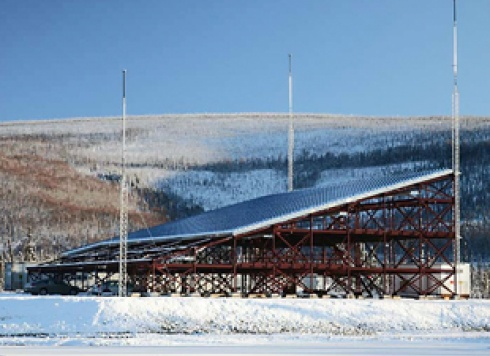
\includegraphics[width=3in]{amisrimage}
\caption{Image of the PFISR \cite{SRIpage}}
\label{fig:amisrpic}
\end{figure}

\subsubsection{Objectives related to 3-D ISR}
There a large number of studies that have used ISR to reconstruct two and three dimensional fields of plasma parameters. Some studies use various types of interpolation to try to stitch together a picture from the one dimensional beams, which give a one dimensional view along range\cite{Semeter2009738,Butler:2013ul,Semeter:2005fo}. Others have taken a tact closer to inverse theory and image reconstruction to create reconstruction of velocity fields of bulk flows or electric fields \cite{butler:imagingfregiondrifts,RDS:RDS20195}. Still, these publications do not get to the core details of reconstructing plasma parameters like the ion and electron temperatures. Interpolations can help visualize the data but these techniques make a lot of assumptions about the underlying imaging process. The goal of this thesis is to present a first principles model of ISR as a three dimensional sensor and use it to create better reconstructions of the plasma parameters.

\subsection{Ionosphere and Phenomena}
The ionosphere is the area of partially ionized gas, or plasma, surrounding the earth, and in a way is like an interface between the earth and outer space \cite{kellybook}. The dynamics of this system are governed by kinetic, fluid and Maxwells equations coupled together \cite{schunk2004ionospheres}. This complicated menagerie of equations allows for the creation of a cornucopia of different phenomena at any number of spatio-temporal scales \cite{Semeter:2008hs,Semeter2009738}.

%In order to understand the behavior of the plasma in the ionosphere one needs to use electromagnetic theory governed by Maxwells Equations seen in Equations \ref{eqn:max1} and \ref{eqn:max2},

%\begin{eqnarray}
%\label{eqn:max1}
%\nabla \cdot \vec{E} = \frac{\rho}{\epsilon_0}\  &&\nabla  \cdot \vec{B} = 0 \nonumber \\
%\nabla  \times \vec{E} = - \frac{\partial B}{\partial t} && \nabla  \times \vec{B} = \mu_{0}\vec{J} +
%\mu_{0}\epsilon_{0}\frac{\partial E}{\partial t}
%\end{eqnarray}
%
%\begin{equation}
%\label{eqn:max2}
%\frac{\partial \rho}{\partial t}+\nabla \cdot \vec{J} = 0
%\end{equation}
% 
%\noindent where $\rho$ is the charge density, $\vec{E}$ is the electric field, $\vec{B}$ is the magnetic field, $\vec{J}$ is the current density, $\mu_0$ is the vacuum permeability and $\epsilon_0$ is the vacuum permittivity. 
%
%In order to close the system of equations often assumptions about the charge density and current density are needed \cite{varnytalk2016}. In the ionosphere though $\vec{J}$ is linked to the electric and magnetic fields, $\vec{E}$ and $\vec{B}$, which are dependent on the particle motion. In the ionosphere these particles move as gas, so to close these systems of equations require the use of fluid and/or kinetic theory depending on what sort of assumptions can be made for the problem.

The study of the Earth's ionosphere is broken up into a number of different regions due to the physical processes that dominate \cite{kellybook}. The demarcations between the D, E and F Regions are based on the altitude, over which various properties of the plasma, including parameters and chemical composition, can greatly vary as shown in Figure \ref{fig:singlefilt} \cite{kellybook}. The regions of the Earth are also parceled out based on the orientation of the magnetic field to the ground and include the high latitude, mid latitude and low latitude regions \cite{schunk2004ionospheres}.

For this thesis most of the focus will be on phenomena from the high latitude F-region. This of special interest due to the number of different phenomena that occur, much of which is due to the perpendicular angle of the Earth's magnetic field to the ground \cite{schunk2004ionospheres}. These phenomena include but are not limited to aurora borealis, polar cap plasma patches and particle precipitation events\cite{Perry:2015jf,Dahlgren:2013ip,dahlgren2012di,Dahlgren:2012dq,semeter:plasmatransport2012}. From a societal standpoint this sort of activity can greatly impact radio propagation and can create interruptions in data services such as the Global Positioning Systems (GPS)\cite{Jiao:2013ei,hunsucker2007high}.


\begin{figure}[!t]
\centering
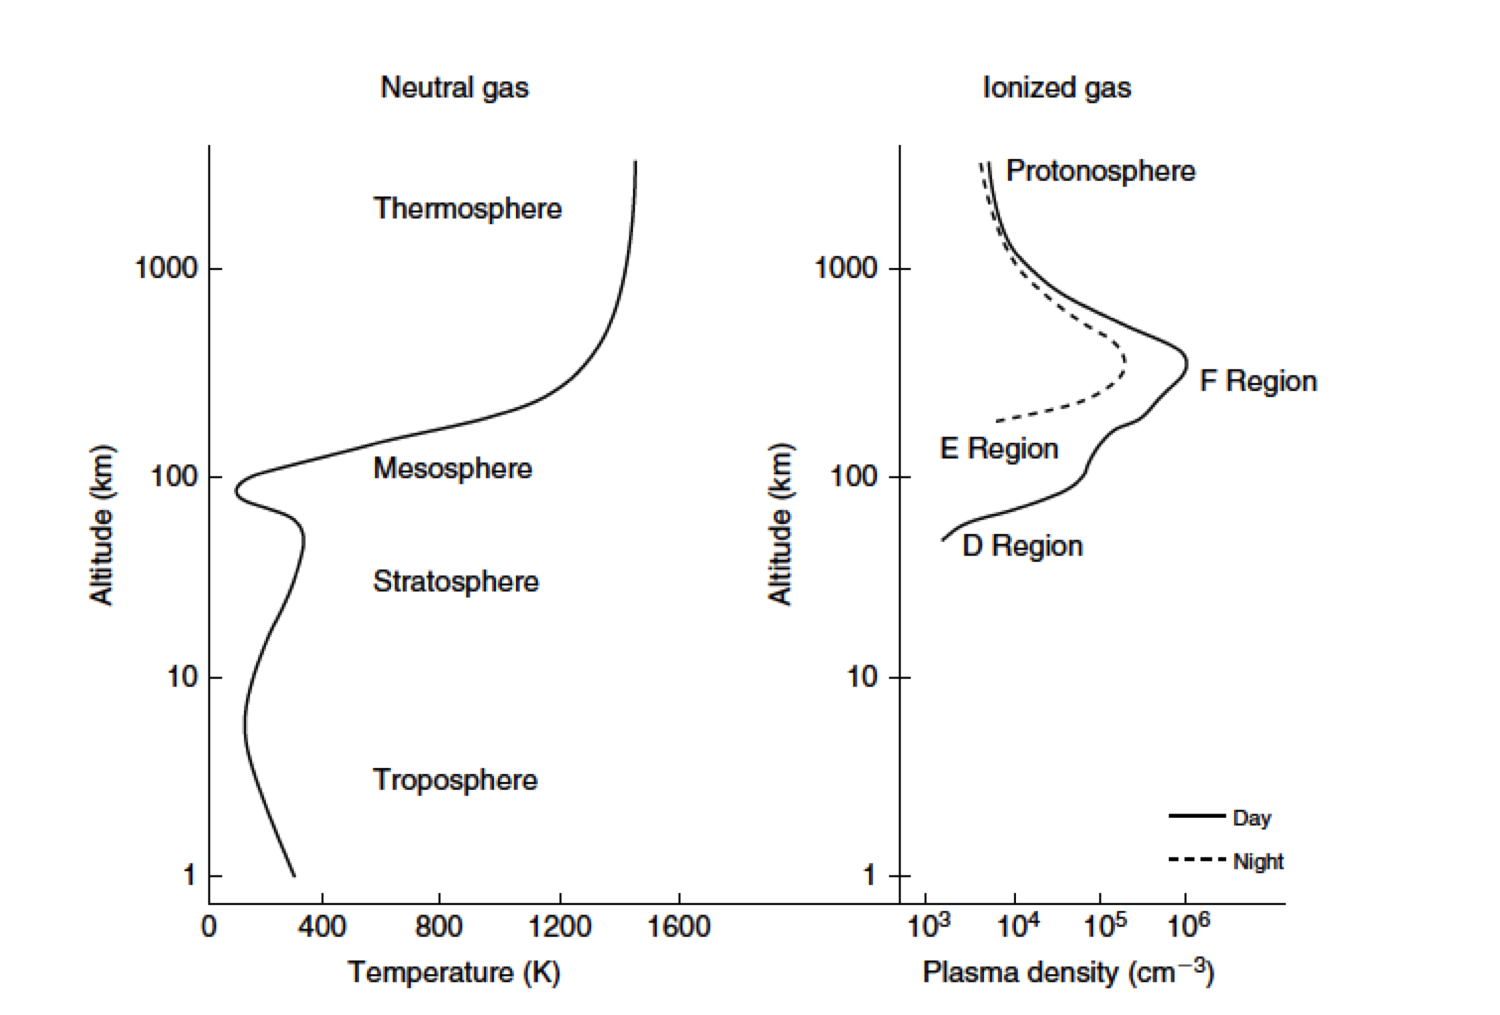
\includegraphics[width=5in]{altvsparams}
\caption{Example profiles of neutral temperature and plasma density from \cite{kellybook}}
\label{fig:singlefilt}
\end{figure}
%These systems right now are all located in what can be considered the high latitude ionosphere.  This is a highly dynamic environment in both time and space.  The plasma can change very quickly due to the physics of the environment.  These types of events can be classified into a number of types that will be of interest to this type of sampling problem.

%\subsubsection{High Spatial Gradient Events}
%Polar cap patches are examples where of high spatial gradients in various plasma parameters \cite{Dahlgren:2012dq,dahlgren2012di}.  In the polar cap large blobs of plasma with elevated electron density travel from the dayside to the night side ionosphere.  These patches can play a large role in plasma transport within the polar ionosphere and interfere with radio transmission as well.  Examples of sensor data that show these patches can be seen in Figure \ref{fig:patches}.
%
%\begin{figure}[!t]
%\centering
%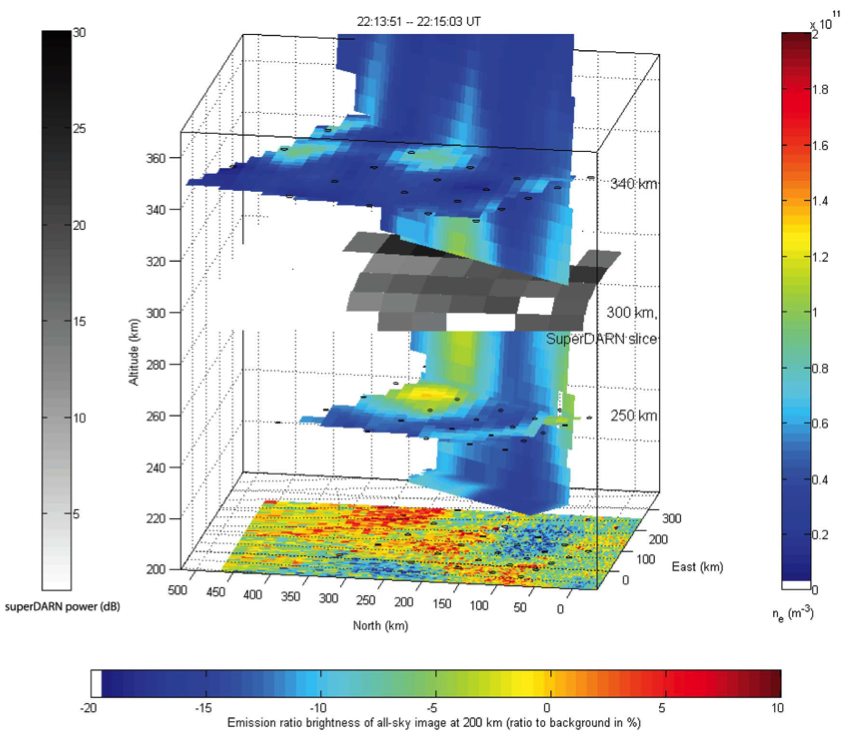
\includegraphics[width=4.0in]{patches}
%% where an .eps filename suffix will be assumed under latex, 
%% and a .pdf suffix will be assumed for pdflatex; or what has been declared
%% via \DeclareGraphicsExtensions.
%\caption{Example of polar cap patches seen in RISR and SuperDARN, from \cite{Dahlgren:2012dq}}
%\label{fig:patches}
%\end{figure}
%
%Large horizontal gradients also occur during geomagnetic storms which can produce large flows.  This can create large disparities in Ion temperature as heating is occurring \cite{Zettergren:2008ba,semeter:plasmatransport2012}.  During these storms ion temperatures can go from 500$^\circ$ K to over 1500$^\circ$ K in the order of kilometers.
%
%These high gradient events can cause some unpredictable errors where two plasma population interface.  These errors can be quite complex due to the nonlinear nature of the inversion process\cite{Vallinkoski1990665}.  Similar behavior has been observed during times of auroral turbulence where shear flows seems to have caused non isotropic temperature measurements\cite{knudsen1993}. 
%%\subsection*{Small Structure Events}
%%\cite{semeter2010CI}
%
%\subsubsection{Dynamic Phenomena}

These phenomena can vary on a multitude of spatio-temporial scales and thus can create difficult sampling problems for sensors tasked measuring them. For the sake of brevity, the rest of the subsection will focus on two examples from the literature and highlight the challenges associated with trying to reconstruct the plasma parameters.

The events shown in \cite{Semeter:2005fo} consist of event known as a poleward boundary intensification (PBI). This occurs when the auroral oval breaks into two separate rings which show a demarcation of different field line configurations in the magnetosphere. The auroral ring closer to the magnetic pole shows a number of strong pulsations which can be seen in both optical and radar data \cite{Semeter:2005fo} .

In the radar reconstruction shown in Figure \ref{fig:Sampling} these events cause large enhancements in electron density that are perpendicular to the ground. These can be challenging to image as these phenomena are moving which can impact how well these events are resolved and ambiguity can be introduced merely in how one processes the data. In this case the researchers found if they integrated fewer pulses per position and allowed for a greater variance in the data they could observe column structuring to the enhancement.

\begin{figure}[htb]
  \begin{minipage}[t]{0.49\linewidth}\centering
    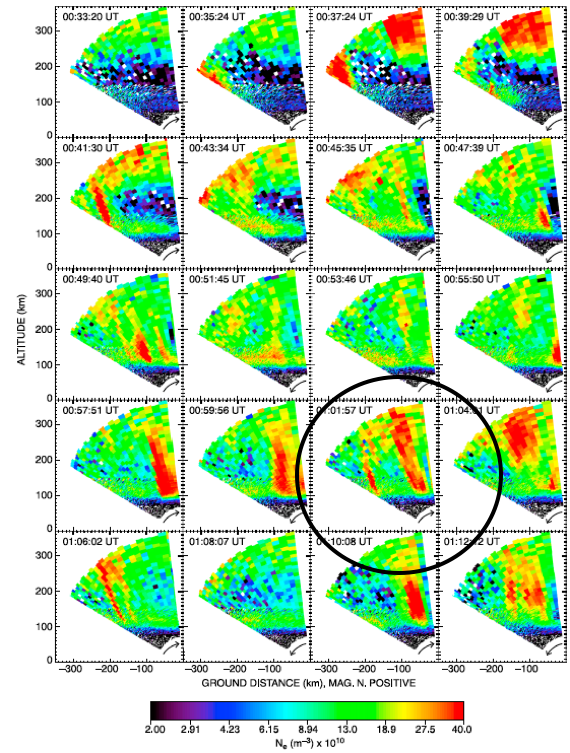
\includegraphics[width=7cm]{pbiall}
    \medskip
    \centerline{(a)}
  \end{minipage}\hfill
  \begin{minipage}[t]{0.49\linewidth}\centering
    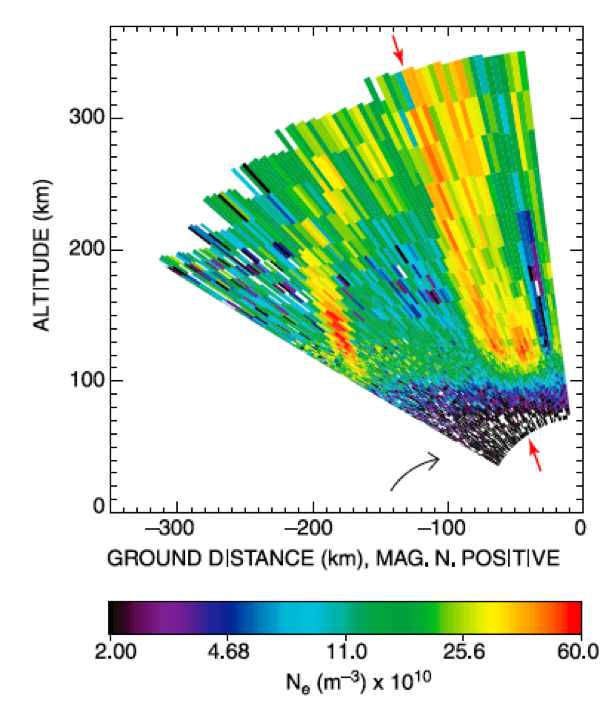
\includegraphics[width=7cm]{pbifast}
    \medskip
    \centerline{(b)}
  \end{minipage}
  \caption{Different views of a poleward boundary intensification event as seen in \cite{Semeter:2005fo}: (a) Data from the Sondastrom processed at 5 seconds; and (b) the same data from the circled frame in b but processed at 2 seconds. }
  \label{fig:Sampling}
\end{figure}

The second phenomena that will be focused on is a sun-aligned auroral arc, specifically from \cite{Perry:2015jf}. These arcs are created by Field Aligned Currents (FAC) from the magnetosphere.The evidence of these structures show themselves in plasma parameters through electron and ion temperature enhancements coincident with electron density depletions next to density enhancements. These structures also are in motion, which can create ambiguities in the measurement process as the plasma moves through the field of view. An example of this type of plasma parameter distribution associated with these types of auroral arcs can be seen in Figure \ref{fig:mzsim}.

\begin{figure}[!t]
\centering
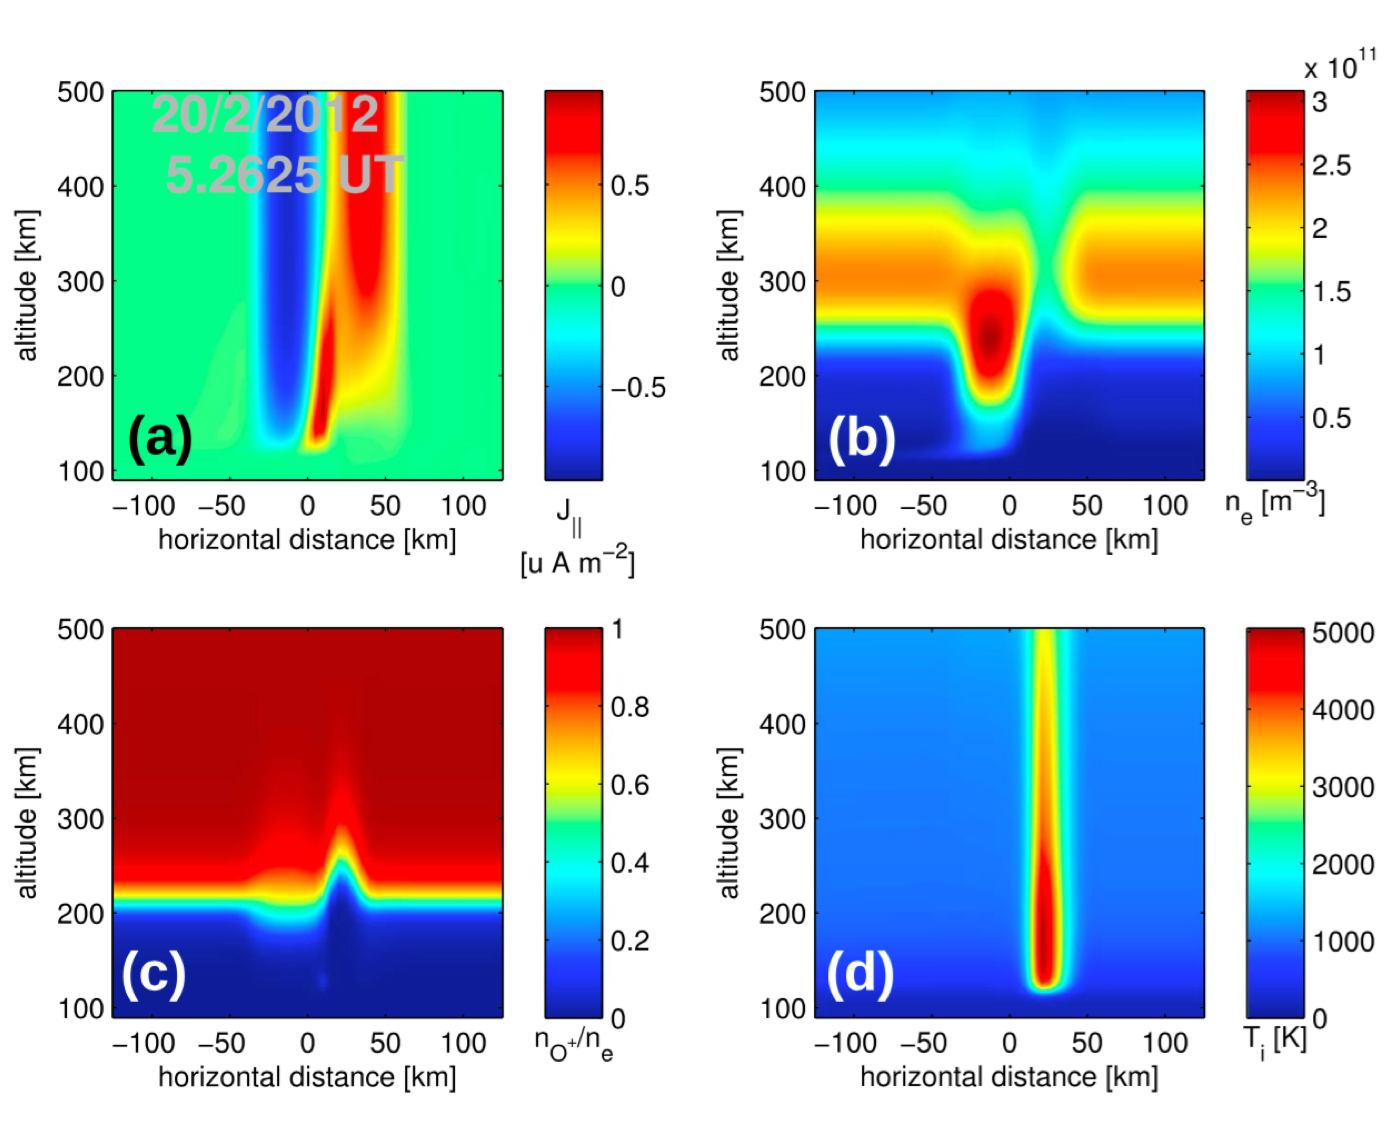
\includegraphics[width=5.0in]{MZsim}
\caption{Image from \cite{Perry:2015jf} showing plasma parameters from a multi-fluid model\cite{semeter:plasmatransport2012} simulating the impact of an auroral arc. }
\label{fig:mzsim}
\end{figure}
%There are also a large number of dynamics and structure found in many auroral events. Using the AMISR system to create volumetric reconstruction of the electron density \cite{Semeter2009738} helped show variability of these events. Figure \ref{fig:eregionact} shows an example of one of these reconstructed events.  Again the like before the researchers again showed the variability during these events by changing the number of pulses integrated and found a large difference in the visible structure.
%\begin{figure}[!t]
%\centering
%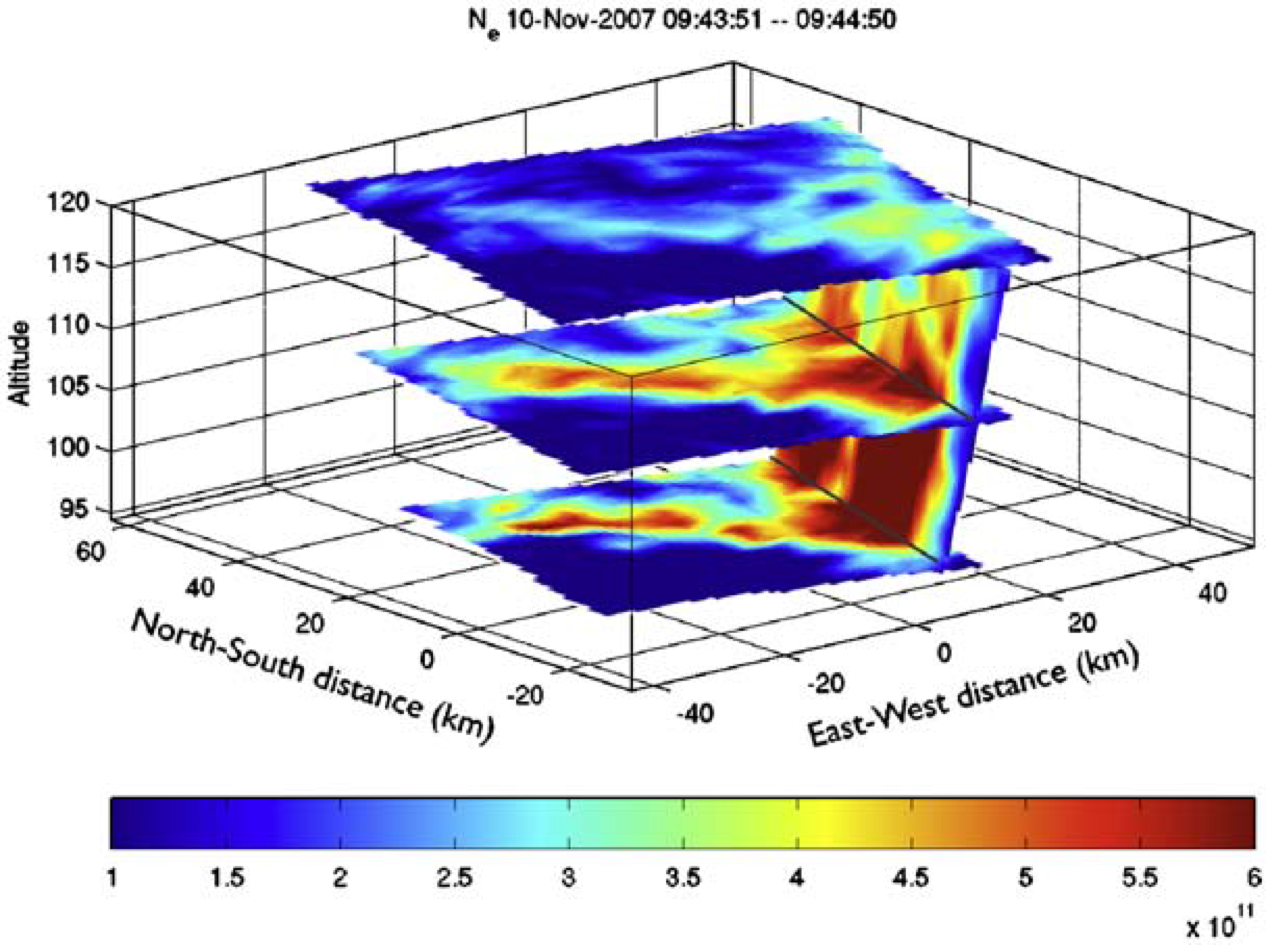
\includegraphics[width=4.0in]{threedamisr}
%\caption{A volumetric reconstruction from AMISR system, from \cite{Semeter2009738}. The reconstruction is of the E-region ionosphere during a auroral precipitation event i.e. electrons following the magnetic field lines of the earth to the lower ionosphere and creating ionization.}
%\label{fig:eregionact}
%\end{figure}
%\subsubsection{High Speed Events}
%At times the ionosphere can be come locally unstable this can create a number of different types of turbulent events. Langmuir turbulence can create coherent structures that will be detected by ISR systems \cite{akbari:2013lt}.  These structures change on the order of one pulse repetition interval of the radar.
%
%Resolving these high speed events are of great interest but also a challenge.  In ISR systems each pulse is used as a sample of a spectral averaging procedure.  It is assumed that these spectrums are identical independent samples.  If spectrum changes during this time, errors in the measurement could take place.  These errors are often unpredictable due to the nonlinear fitting used to fit the spectrum with the plasma parameters.
 %\cite{Dahlgren:2013ip}
%In the past researchers have studied errors associated with different plasma distributions mixing together.  These errors can be quite complex due to the nonlinear nature of the inversion process\cite{Vallinkoski1990665}.  Similar behavior has been observed during times of auroral turbulence where shear flows seems to have caused non isotropic temperature measurements\cite{knudsen1993}. 
\subsubsection{Objectives related to the Phenomena of the Ionosphere}
The main goal of using ISR is to get the most accurate reconstructions of plasma parameters possible. This research creates a framework with which researchers can use to improve their experiment planning. This frame work includes a simulator that can create synthetic ISR data which they can use to try different experiment set ups and reconstruction methods. The simulation examples parameter distribution derived or directly from those shown in Figures \ref{fig:Sampling} and \ref{fig:mzsim} as phantoms to test the reconstruction methodology.

\subsection{Image Reconstruction}
\label{sec:imgrec}
Inverse theoretic image reconstruction gives engineers and scientists a robust frame work to determine the state of system parameters given a data set. This sort of frame work has been applied to numerous problems in science and engineering from X-Ray computed tomographic scanning \cite{kak1988principles} to synthetic aperture radar \cite{1456966}. In this thesis we will use this framework and techniques to improve the quality of the plasma parameter estimates from ISR.

The main gaol of image reconstruction and inverse theory is to reconstruct a set of parameters given a set of data using knowledge of the forward model. Using the notation found in \cite{menke2012geophysical} a general inverse problem can be stated as follows,

\begin{equation}
\label{eqn:invprob}
\mathbf{d}=\mathbf{g}(\mathbf{m})
\end{equation}

\noindent where $\mathbf{d}$ is the data $\mathbf{g}$ is the operator that changes the parameters $\mathbf{m}$ to the data space. 

Although Equation \ref{eqn:invprob} gives a general framework this problem can be difficult to solve. Often, techniques used to solve inverse problems entail some assumption that can be made about the operator $\mathbf{g}$ such as linearity or that its well-posed \cite{0266-5611-4-4-010}. Still there are ways to get around this by doing things such as adding constraints or regularization to the inversion method \cite{Vogel:2002:CMI:581830}.

ISR has in past been presented in this format, although this has mainly been for the case of a single beam \cite{Vierinen:2012ve}. ISR can be thought of a general inverse problem because of the non-linear operation that brings the plasma parameters to the ACF space. Two schools of thought have emerged which in the community on how to be constrain these inversions. The first, full profile analysis, uses plasma parameter constraints, which can give physical constraints to the inversion thus improving the outcome \cite{hysell2008,RDS:RDS3308}. The second set of techniques apply constraints on the estimated ACFs \cite{Virtanen:20082vx,nikoukar2008}, which is less expensive computationally but can create ACFs that cannot be created through IS theory.

\subsubsection{Objectives related to the image reconstruction}
This thesis will couch the estimation of 3-D ISR in the language of inverse theory. It will use techniques to improve the accuracy of the reconstruction of plasma parameters.

\subsection{Outline of dissertation}

Chapter \ref{chapter:isrproc} will go into the background into ISR signal processing. This will be begin by developing the basic signal model and show the processing steps between the sampling complex voltages to plasma parameter measurements.

Chapter 3 will show the derivation of space-time ambiguity function. This will allow for the posing reconstruction of the field of three dimensional plasma parameters in the language of inverse theory. 

Chapter 4 contains a discussion of the frame behind the Simulator for ISR (SimISR). This simulator can create complex voltages and process the data. This can help plan experiments the future. This will also include the examples of simulated data to show the capabilities of this framework.

Chapter 5 will detail an inversion method that has been developed to reduce the impact of the space-time ambiguity. This inversion method allows for plasma parameter reconstructions along the frame of reference of the moving plasma.

\section{Contributions}
Specific contributions of this research are summarized below.

\begin{enumerate}
\item Development of a theoretical framework for the forward model of 3-D ISR plasma parameter reconstructions.
\item Creating a framework full simulation of an ISR system that can which yield synthetic complex voltages.
\item A software package, named SimISR has be derived from previously mentioned simulation framework has been made available to other researchers.
\item A detailed analysis of the simulation framework using SimISR.
\item A new method for inverting the forward model for 3-D ISR plasma parameter reconstructions.
\end{enumerate}
\cleardoublepage

% -------------------------------------
% CHAPTER 2: ISR Processing
% -------------------------------------
\chapter{Incoherent Scatter Radar Signal Model \& Processing}
\label{chapter:isrproc}
\thispagestyle{myheadings}

% set this to the location of the figures for this chapter. it may
% also want to be ../Figures/2_Body/ or something. make sure that
% it has a trailing directory separator (i.e., '/')!
\graphicspath{{2_ISRProc/Figures/}}

%%%%%%%%%%%%%% Intro %%%%%%%%%%%%%%%%%%%%%%%%%%%%%%%%%%%%%

This chapter will give the background on the signal model and processing aspects of ISR. The first section will explore the physical  underpinning of the incoherent scatter signal from the ionosphere. The second section will detail the basics of radar processing and how the different types of measurements are made. In the final section of this chapter the specific processing that takes place in an ISR will be detailed.

\section{Incoherent Scatter}
\label{sec:incohscat}
When electrons are freed from their bonds as in a plasma they can oscillate in a manner modeled as a dipole antenna. If an electromagnetic wave, such as one from a radar pulse, impinges on these electrons they will accelerate and re-radiate a wave. This scattering process is known as Thomson scatter \cite{Hutchinson_2002}. This radiation, when taken as a collection of scatterers from a large set of electrons, varies in time $t$, with fluctuations in electron density $n_e(\mathbf{k},t)$, where $\mathbf{k}$ is the Bragg vector \cite{kudeki:milla:1}. In the far-field condition the Bragg vector is defined as
\begin{equation}
\label{eqn:bragg}
\mathbf{k}=\mathbf{k}_s-\mathbf{k}_i,
\end{equation}
where $\mathbf{k}_s$ and $\mathbf{k}_i$ are the wavenumbers for scattered and incident waves respectively \cite{sheffield2010}. The Bragg vector is the frequency parameter in $n_e(\mathbf{k},t)$, where the spatial Fourier transform $n_e(\mathbf{r},t)$ has position vector $\mathbf{r}$. As these charges move the scattered waves are given a Doppler shift based off of their velocity, $\mathbf{v}$ along the Bragg vector. This Doppler shift in frequency can be represented as
\begin{equation}
\label{eqn:dop1}
\omega=\mathbf{k} \cdot \mathbf{v},
\end{equation}
where $\omega$ is the frequency shift from the velocity along the Bragg vector \cite{sheffield2010}. $n_e(\mathbf{k}, \omega)$ can be thought of as both the Fourier Transform along time of $n_e(\mathbf{k},t)$ and the collective Doppler spectrum from the density at a specific Bragg vector $\mathbf{k}$.

These fluctuations are driven by the random thermal motions of the electrons and the collective radiation they create is known as incoherent scatter \cite{kudeki:milla:1}. Another term for this is \textit{non-collective} scattering with relation,
\begin{equation}
\label{eqn:incohorig}
k*\lambda_{e} << 1,
\end{equation}
where $\lambda_{e}$ is the electron Debye length, and $k=|\mathbf{k}|$. This will cause the spectrum to show the collective effects of the velocity distribution of the particles \cite{sheffield2010}.
Although the scattering is driven through a random process it reveals several pieces of information about a plasma, especially in the ionosphere. Due to the electrical interaction between the ions and electrons a correlation structure develops, creating a shaped Doppler spectrum that a radar can detect. This Doppler spectrum is a power spectral density estimate of the electron density fluctuations across time $t$ and $\langle \left|n_e(\mathbf{k},\omega)\right|^2\rangle$.

The IS spectrum has a number of different sections separated in frequency.
This thesis focuses on the ``ion line'' portion of the spectrum shown in Figure~\ref{fig:ispecch2}. This naming is due to the IS spectrum revealing a damped version of ion acoustic waves
\begin{equation} 
\label{eqn:ial}
\omega=k_0\sqrt{\frac{K_b(T_e+3T_i)}{m_i}}
\end{equation}
where $k_0$ is the wavenumber, $\omega$ is the radian frequency of the wave, $K_b$ is Boltzman's constant, $m_i$ is the mass of the ion species and $T_e$ and $T_i$ are the temperatures of the electron and ions \cite{chen1984introduction}. 
The ion acoustic mode returns the most power and can give information on both electron and ions, so it is commonly used in ISR analysis.

The physical intuition behind the ``ion line'' can useful for understanding basic processes, but a full mathematical model tying plasma parameters, such as electron density ($N_e$), electron temperature ($T_e$),  and ion temperature ($T_i$) to the power spectral density ($\langle \left|n_e(\mathbf{k},\omega)\right|^2\rangle$) is necessary for ISR to perform its measurements. There have been a number of derivations and formulations for this since the development of ISR \cite{dougherty:farley1960,farleydougherty:ISR2,doughteryfarley:ISR3,hagfors1961}. This thesis will use the formulation from~\cite{kudeki:milla:1,kudeki:milla:2,Kudeki:2006kx},
\begin{equation}
\label{eq:mainspeceq:body}
\langle \left|n_e(\mathbf{k},\omega)\right|^2\rangle = \frac{|j\omega\epsilon_0 + \sigma_i|^2 \langle |n_{te}(\mathbf{k},\omega)|^2\rangle}{|j\omega\epsilon_0 +\sigma_e+\sigma_i|^2} + \frac{| \sigma_e|^2 \langle |n_{ti}(\mathbf{k},\omega)|^2\rangle}{|j\omega\epsilon_0 +\sigma_e+\sigma_i|^2}.
\end{equation}
The overall spectra from the collective effects of the electrons and different species of ions is made up of the weighted superposition of independent fluctuation spectra for each species $\langle |n_{ts}(\mathbf{k},\omega)|^2\rangle$. The weightings are made up of the longitudinal conductivities of each species $\sigma_s$, the frequency $\omega$ and $\epsilon_0$ is the vacuum permittivity. 

The independent fluctuation spectra and conductivities are related to plasma parameters through Gordeyeve integrals $J_s(\omega)$, specifically 
\begin{equation}
\label{eq:thermalfl:bod}
\frac{\langle|n_{ts}(\mathbf{k},\omega)|^2\rangle}{N_s} = 2\text{Re}\{J_s(\omega)\},
\end{equation}

\noindent and 
\begin{equation}
\label{eq:cond:bod}
\frac{\sigma_{s}(\mathbf{k},\omega)}{j\omega\epsilon_0} = \frac{1-j\omega J_s(\omega)}{k^2\lambda_s^2},
\end{equation}
where $N_s$ is the average density for the species, and $\lambda_{e}$ is its Debye length. The Gordeyeve integrals are the one sided Fourier transforms of the characteristic functions of the particle displacements $\langle e^{j\mathbf{k}\cdot\Delta\mathbf{r}_s}\rangle$, or  
\begin{equation}
\label{eq:gord:body}
J_s(\omega)\equiv \int_0^\infty \langle e^{j\mathbf{k}\cdot\Delta \mathbf{r}_s}\rangle e^{j\omega\tau}d\tau.
\end{equation}
For the case of a Maxwellian distributed plasma where collisions and magnetic field can be neglected,
 \begin{equation}
\label{eq:pdfallc2}
\langle e^{j\mathbf{k}\cdot\Delta \mathbf{r}}\rangle= e^{-\frac{1}{2}k^2C^2 \tau^2},
\end{equation}
where $C=\frac{K_bT_s}{m_s}$, $T_s$ is the temperature of the species, $K_b$ is Boltzmans constant and $m_s$ is the mass of the species in kg.

This formulation can also allows for the measurement of bulk of the plasma. This measurement is along the radars wave vector and results in the substitution of $\omega_s=\omega-\mathbf{k}\cdot\mathbf{V}_s$, where $\mathbf{V}_s$ is the bulk motion of the plasma species, into the Gordeyve integrals in Equation~\ref{eq:gord:body} for $\omega$. Generally all of the species will flow together, otherwise large electric fields would form, and this overall motion can be measured as a overall shift of the spectrum in frequency.

A more complete treatment of the IS spectrum formulation, derivation and computational considerations is given in Appendix~\ref{appendix1}. An example of ion line portion of the IS spectrum, with  $|\mathbf{k}|=18.5$ rad/m and using parameters representative of the F-region ionosphere, is shown in Figure \ref{fig:ispecch2}. 
% make ISR spectra
\begin{figure}[htb]
\centering
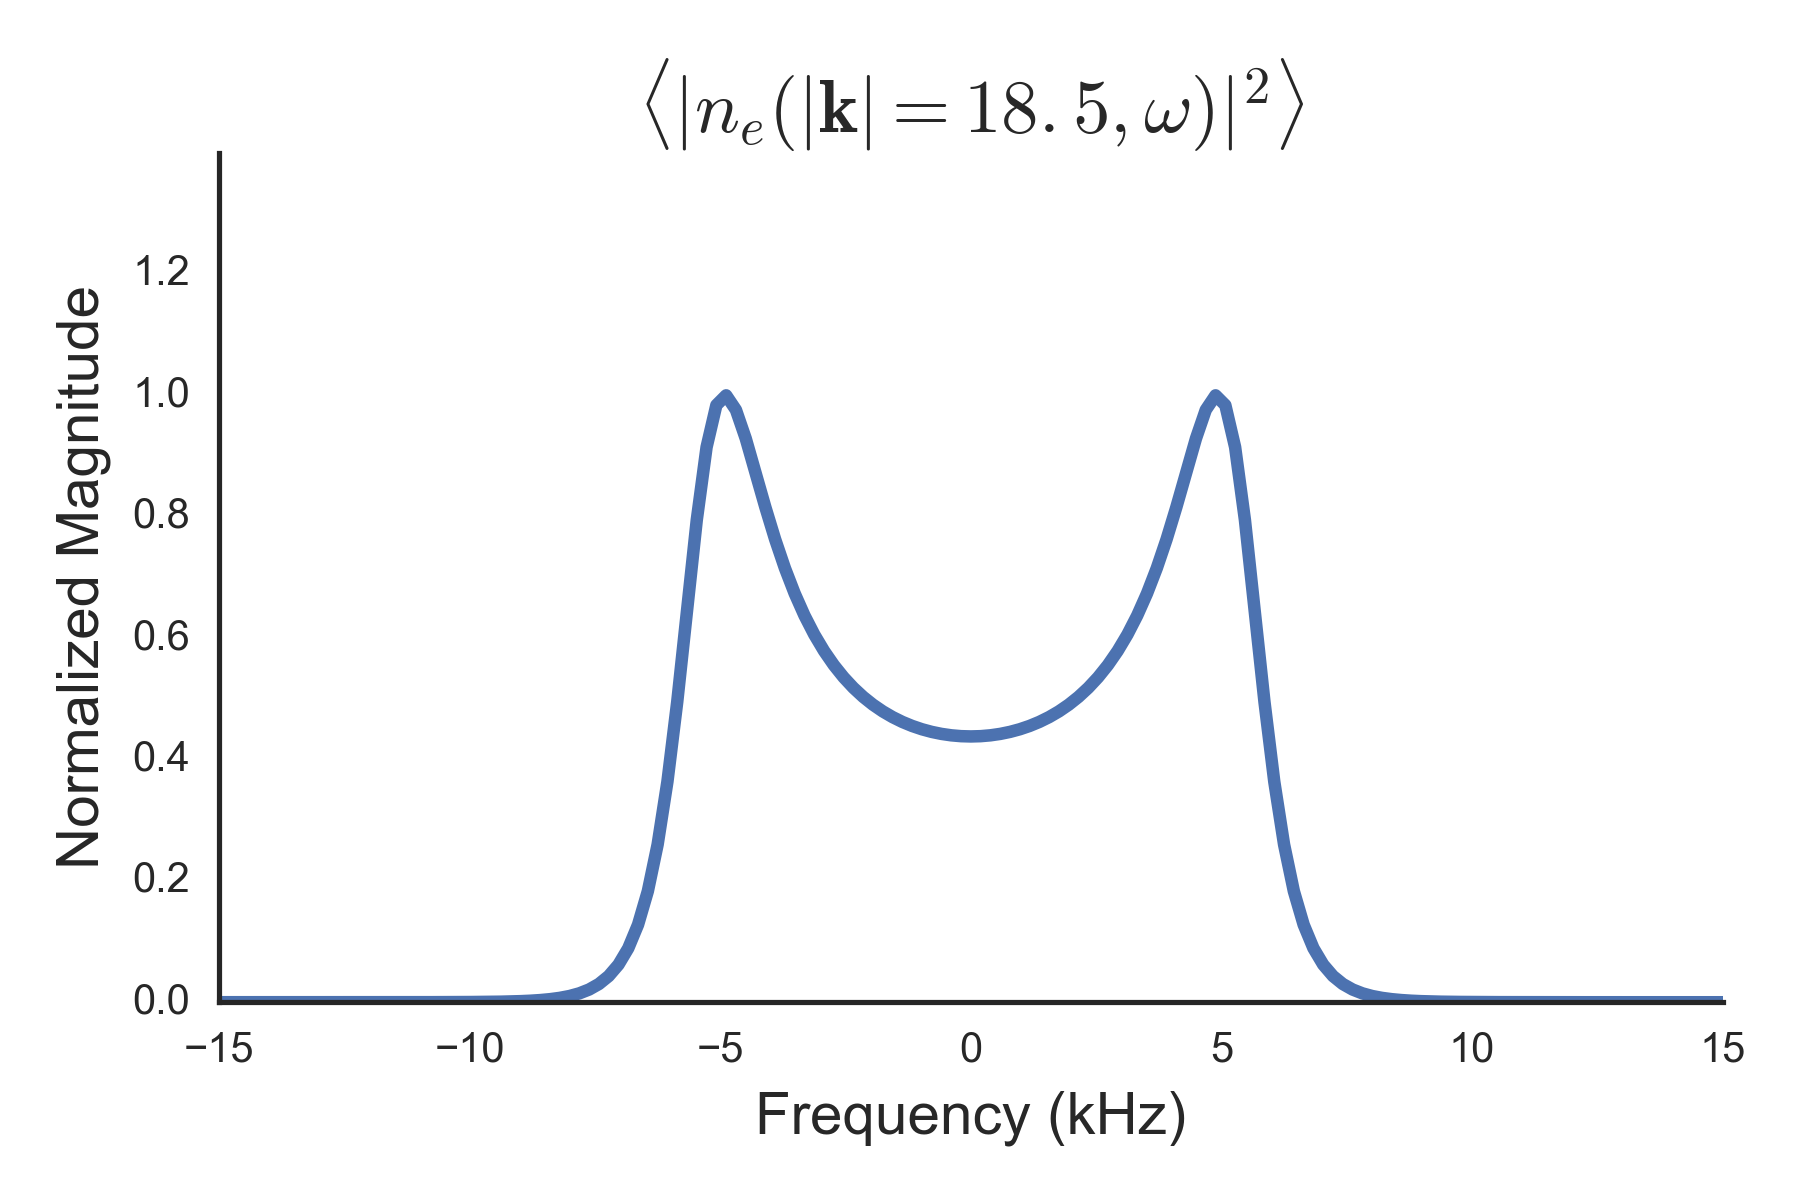
\includegraphics[width=4in]{Specion}
\caption{IS spectrum ion line with all O$^+$ ions, $N_e = 10^{11}$, $T_e=2500 ^\circ$ K and $T_i=1000 ^\circ$ K. }
\label{fig:ispecch2}
\end{figure}

As its name implies, IS is inherently stochastic in nature. To measure this spectrum with usable error margins a number of observations of this process must be averaged together \cite{Diaz:2008co}. Common ISR analysis practice refers to observations of this random process as ``pulses," to distinguish this from samples in signal processing applications \cite{dtsp:openhiem}. These observations can then be used in some sort of spectral estimator . A demonstration of the convergence of a periodogram estimator to the spectrum from Figure \ref{fig:ispecch2} as the number of pulses $J$ is increased is depicted in Figure \ref{fig:ispecch2ave}.
\begin{figure}[htb]
\centering
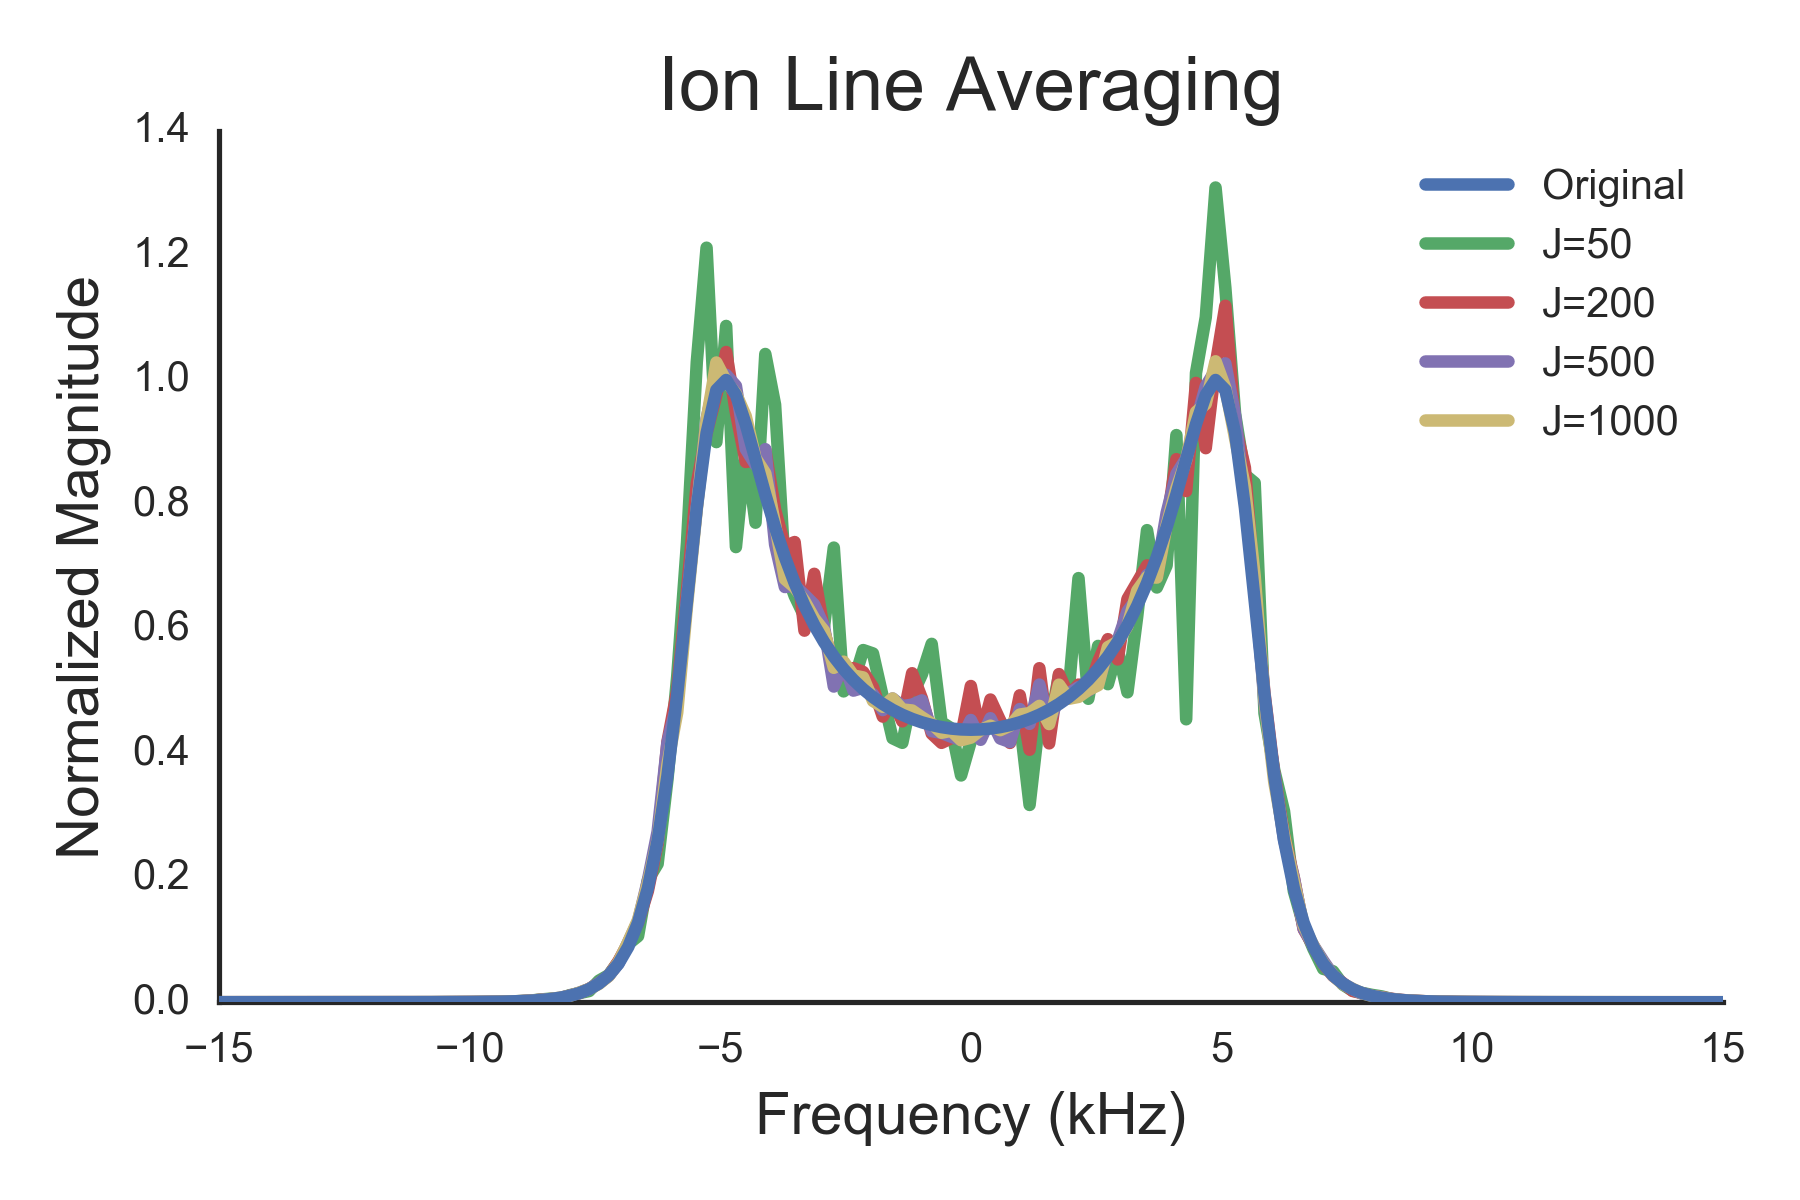
\includegraphics[width=4in]{Specionave}
\caption{IS spectrum ion line with all parameters from Figure \ref{fig:ispecch2} with, number of observations or pulses $J =$ 50, 100, 500 and 1000 averaged together using a periodogram estimator. }
\label{fig:ispecch2ave}
\end{figure}

\section{Radar Signal Processing}

In this section the general signal model behind ISR will be discussed. Following that the specifics of measuring a Doppler spectra, like the IS spectrum will be covered. Some comparisons to hard-target radar systems will be made as well.

\subsection{Radar Signal Model}
ISR systems like other pulsed radar systems radiate a signal, $y(t)$, that can be represented as a finite length pulse, $s(t)$ modulated by a complex sinusoid
\begin{equation}
\label{eqn:sigone}
y(t)=s(t)e^{j2\pi f_0 t}
\end{equation}
where $f_0$ is the transmit frequency in Hz. Equivalently, $ f_0=c/\lambda_0$, where $\lambda_0$ is the wavelength of the transmitted wave and $c$ is the speed of light. The return signal reflected off of a single point target, which assuming for now has no motion may be modeled as
\begin{equation}
\label{eqn:sigone}
y_r(t)=A_0s(t-\Delta t)e^{j2\pi f_0 (t-\Delta T)}
\end{equation}
where $\Delta T$ round trip time and $A_0$ is a complex amplitude factor including propagation losses, phase shifts and target reflectivity \cite{richards2014fundamentals}. The radar system estimates the range $r$, or the distance between the target and sensor,
\begin{equation}
\label{eqn:range_intro}
r=\frac{c\Delta T}{2}.
\end{equation}
Lastly, the signal is demodulated down to baseband, becoming
\begin{equation}
\label{eqn:baseband}
x(t)=A_0s(t-\Delta T)e^{-j2\pi\Delta T}.
\end{equation}

Another key quantity estimated by ISR is the line of sight, or bulk Doppler velocity. The Doppler for this specific case acts as multiplication of the radar signal $s(t)$ with a simple single complex exponential
\begin{equation}
\label{simpledop}
s_d(t) = s(t)e^{j2\pi f_d t},
\end{equation}
 where $f_d$ is the Doppler frequency of the target and $s_d(t)$ is the received signal in~\ref{eqn:baseband} with a Doppler shift. Assuming there are no relativistic effects this frequency can be represented as the following $f_d = 2v/\lambda_0 $, where $v$ is the velocity of the target. 

With ISR a distribution of electrons are probed, so we have an extremely large number of small cross-section targets within the beam. A better model would be a set of scatterers each with their return weighted ($V_n$) and with a frequency shift, ($f_n$), represented as
\begin{equation}
\label{multiDop}
\displaystyle s_d(t) = \sum_{n}^{N} s(t)V_ne^{j2\pi f_{n} t},
\end{equation}
For very large $N$ number of scatterers this model can be extended to a continuum of signals, becoming
\begin{equation}
\label{conDop}
s_d(t) = \int s(t) V(f)e^{j2\pi ft} df.
\end{equation}

A simple illustration of the sampling is shown in Figure \ref{fig:isrfigure} which shows range-time diagram for ISR. In this case three samples are taken from different ranges and the pulse, $s(t)$ is multiplied by the electron density fluctuations $n_e$ at its corresponding time and range. The return signal $x$ is sampled with a period of $T_s$  making sample values at times $t_1$, $t_2$ and $t_3$. 
\begin{figure}[htb]
\centering
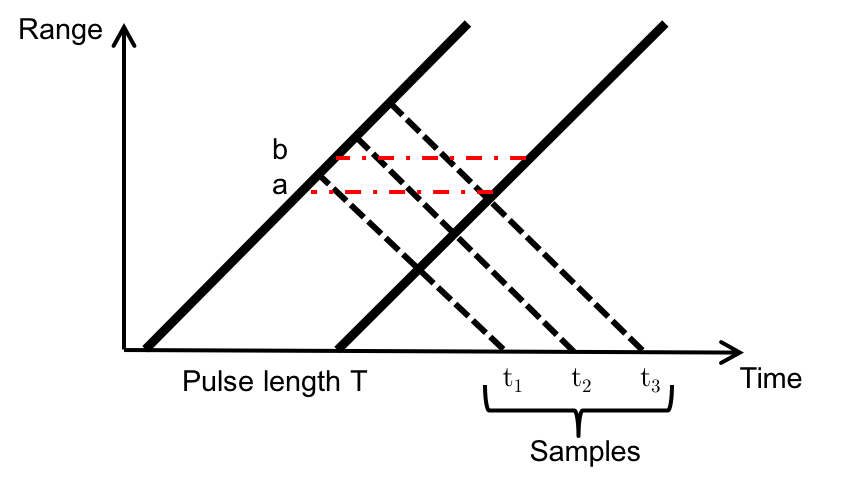
\includegraphics[width=5in]{ISRpicture}
\caption{As the pulse in time traverses the ranges a, b, and c, it is multiplied by the electron density fluctuations at each of those points. The samples at each time are the summations of those returns from each point that the lines intersect in range. These different points are also delayed in time as well giving time delayed observations of the process at each point. }
\label{fig:isrfigure}
\end{figure}
sample values $x(t)$ at each point can be seen in Equation \ref{eqn:isrbrokenout}.
\begin{equation}
\label{eqn:isrbrokenout}
\begin{split}
 x(t_1)=& n_e(\text{a},t-\text{a}/c)s(t-2\text{a}/c) \\ 
 x(t_2)=& n_e(\text{a},t-\text{a}/c-T_s)s(t-2\text{a}/c-T_s) +  n_e(\text{b},t-\text{b}/c)s(t-2\text{b}/c)\\
 x(t_3)=& n_e(\text{a},t-\text{a}/c-2T_s)s(t-2\text{a}/c-2T_s)   +
 \\ & n_e(\text{b},t-\text{b}/c-T_s)s(t-2\text{b}/c-T_s) 
 \end{split}
\end{equation}

The terms in Equation \ref{eqn:isrbrokenout} are single points in range from Equation~\ref{eqn:xwithne} which is the common formulation of the return data for ISR \cite{hysell2008}, 
\begin{equation}
\label{eqn:xwithne}
x_c(t)= \int n_e(r,t-r/c)s(t-2r/c)  dr.
\end{equation}
By performing a change of variables it should be noted that Equation \ref{eqn:xwithne} has the same form as Equation~\ref{eqn:timevarfilt}
\begin{equation}
\label{eqn:timevarfilt}
x_c(t)= \int h(\tau,t)s(t-\alpha\tau)  d\tau,
\end{equation}
where $h(\tau,t)$ is a filter with an impulse response along $t$ varies with $\tau$ and $\alpha$ is a translation so the time steps between $t$ and $\tau$ are equal.  One of the earlier uses of model  form comes from the study of time varying communication channels \cite{Kailath:1962jx,Kailath:1963gh}. This time-varying filter model can help determine the method of measurement by looking at the Fourier Transform of $h(\tau,t)$,
\begin{equation}
\label{eqn:timvarefreq}
H(\tau,f)=\int h(\tau,t)\text{e}^{-j2\pi ft}dt.
\end{equation}
The term $H(\tau,f)$ is known as the time-varying frequency response, which can be used to determine how the function can be measured and does this by distinguishing two different target classes. The first class, an \textit{underspread} target the following inequality must hold,
\begin{equation}
\label{eqn:trp}
BL<1,
\end{equation}
where $B$ is the bandwidth of $H(\tau,f)$ and $L$ is its extent along $\tau$ \cite{Kay:2003jl,Pfander:2015ea}. The second class, the \textit{overspread} target, occurs when this inequality does not hold.

With ISR this same frame work can be used, the term $L$ must now change to $R_L/c$ where $R_L$ is the farthest range that needs to be probed. In the case of ISR probing the F-region the target is overspread as the inequality in Equation \ref{eqn:trp} will not hold. In order to estimate the time-varying frequency response an ambiguity will be introduced \cite{Kailath:1962jx,Kailath:1963gh}, which is the same as performing the measurement of the Doppler spectrum. This discussion of \textit{overspread} vs. \textit{underspread} will drive the Doppler measurement methodology discussed next.




\subsection{Doppler Measurement}
In a pulsed radar system Doppler is measured starting with these steps:
\begin{enumerate}
\label{list:uno}
\item radar sends a set of pulses that scatter off the targets 
\item target returns are binned into a two-dimensional array representing range and interpulse period (IPP).
\end{enumerate}
In the case of an \textit{underspread} target the pulse-Doppler processing method can be used, which is commonly denoted \textit{coherent processing} \cite{richards2014fundamentals,richards2010principles,richards2014principles,skolnik2008radar}. The pulse-Doppler method consists of the following steps after the first two listed:
\begin{enumerate}
  \setcounter{enumi}{2}
  \item a discrete Fourier transform (DFT) across pulses is taken to determine the Doppler spectrum \cite{richards2014fundamentals}. 
\item A power spectrum is formed by taking squared magnitude .  
\end{enumerate}

In order to avoid aliasing or Doppler folding, the pulse repetition frequency (PRF) must be at least twice as large as largest Doppler frequency in the signal \cite{dtsp:openhiem}. 
a phase-coherent signal that is relatively narrow in frequency can obtain a large amount of gain compared to the background noise. The Doppler bandwidth that can be view unambiguously will be tied to the PRF. The issue of range ambiguity can arise if the support of the target is further in range than a single pulse can travel in an IPP. The maximum unambiguous range, $R_a$, can be represented as 
\begin{equation}
\label{eqn:maxuar}
R_a =  \frac{cT}{2}
\end{equation}
where $T$ is the IPP time. These requirements fit within the definition of an  \textit{underspread} target, thus pulse-Doppler processing assumes this class of target.

The ionosphere is not compactly supported in range if one wants to do F-region studies, which can stretch from 150-700 km in altitude. 
Using the spectrum in Figure~\ref{fig:ispecch2}, it can be seen that the signal is at least 20~kHz in bandwidth.
This broad bandwidth and unambiguous range requirement yields an \textit{underspread} target. 

In order to measure an this class of target, an alternative Doppler processing method must be used. This method replaces steps \#2 and \#3 with an estimate of the autocorrelation function (ACF) within the IPP and a DFT across the lags is taken to get the Doppler spectrum.
The formation of this spectrum is the same as forming Wigner-Ville distribution along range \cite{TFAcohen}. The formulation of the Wigner-Ville distribution is as follows using a signal $x(t)$,
\begin{equation}
\label{eqn:wigdist}
W_x(t,f)=\int x_c(t-\tau/2)x_c^*(t+\tau/2)\text{e}^{-j2\pi \tau f}d\tau,
\end{equation}
where $\tau$ is the lag variable. Because phase coherency is not needed across pulses this is considered an \text{incoherent processing} technique \cite{richards2014fundamentals,richards2010principles,richards2014principles,skolnik2008radar}. 
Note that ISR received its name due to the physical definition of incoherent scatter as explained in Section \ref{sec:incohscat} \cite{gordon58,dougherty:farley1960}.


In the specific case of ISR processing for an uncoded pulse the processing follows this logic and performs an approximation to the formation of the Wigner-Ville distribution, which will be examined in the next section. 


%%%%%%%%%%%%%% Processing %%%%%%%%%%%%%%%%%%%%%%%%%%%%%%%
\section{ISR Processing}\label{section:isrproc}
The specifics of ISR processing will be discussed in this section. It will mainly use the terminology found in much of the ISR literature~\cite{farley1969,nygren1996}. This examination of the processing will start after complex receiver voltage data have been received, and detail how it is processed to create estimates of the ACF at desired points of space.

 
The processing follows the flow chart presented in Figure~\ref{fig:chain}.  
Note that we assume here a signal pipeline which creates a single altitude measurement for analysis. 
More sophisticated approaches for ISR analysis exist that use information from multiple altitudes, including full profile analysis \cite{RDS:RDS3308}, lag profile inversion \cite{Virtanen:20082vx}, and others, but treatment of these approaches is beyond the scope of this chapter.
\begin{figure}[!t]
\centering
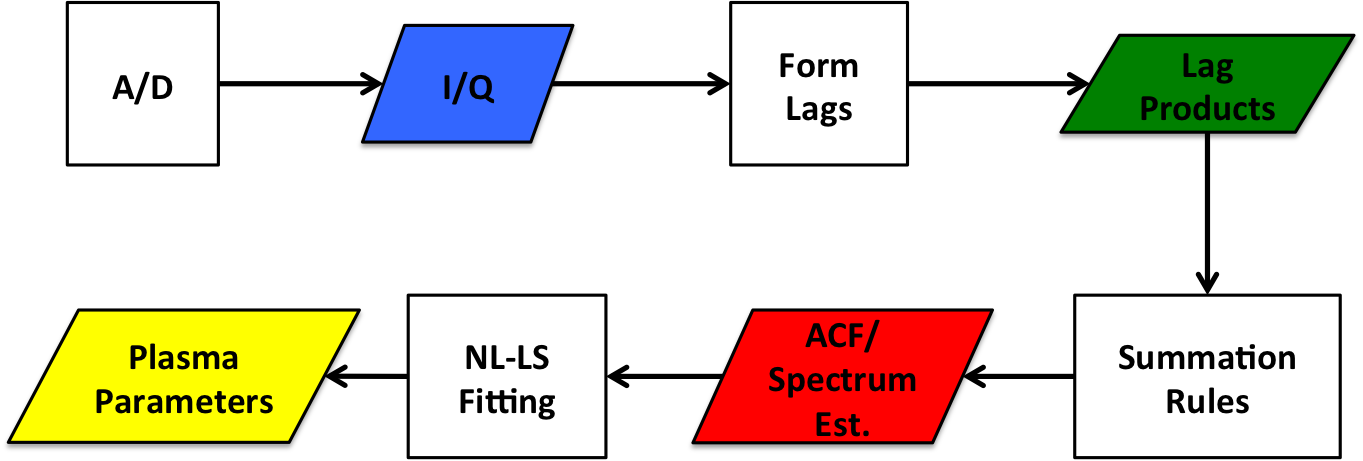
\includegraphics[width=5.5in]{datastackchain}
\caption{ISR signal processing chain, with signal processing operations as squares and data products as diamonds.}
\label{fig:chain}
\end{figure}
The lag product formation is an initial estimate of the autocorrelation function. The sampled complex receiver voltage can be represented as $x(n) \in\mathbb{C}^N$ where $N$ is the number of samples in an inter-pulse period. For each range gate $m\in 0,1,...M-1$ a complex autocorrelation is estimated for each lag of $l \in 0,1...,L-1$. To keep the number of integrated samples for each lag the same across all of range, the number of range gates for each IPP will be at most $N-(L-1)$. To get better statistics this operation is performed for each pulse $j\in 0,1,...J-1$ and then summed over $J$ independent pulses. The entire operation to form the initial estimate of $\widehat{R}(m,l)$ may be expressed as

\begin{equation}
\label{eq:lagpro}
\widehat{R}(m,l) = \displaystyle\sum\limits_{j=0}^{J-1} x(m-\lfloor l/2\rfloor,j)x^*(m+\lceil l/2 \rceil,j).
\end{equation}

The case shown in Equation \ref{eq:lagpro} is a centered lag product.  Other types of lag product calculations are available but a centered product is most common. For this case, the range gate index $m$ and sample index $n$ can be related by $m=n-\lfloor L/2\rfloor$ and the maximum lag and sample relation is $M=N-\lceil L/2 \rceil$.  This lag product formation is the first step in computing a discrete Wigner Distribution \cite{TFAcohen}. This  step adds a bias to the ACF estimate which acts as a weighting on larger lags, represented as $\mathcal{W}(l)$ where weighting can be calculated from details of the range-lag ambiguity function. The expected value for the estimator, assuming the use of a simple uncoded pulse waveform, becomes

\begin{equation}
\label{eq:lagprobias}
\left\langle\widehat{R}(m,l) \right\rangle = \mathcal{W}(l)R(m,l) =\frac{L-l}{L}R(m,l).
\end{equation}

%This specific type of lag product formation is detailed in \cite{farley1969} and had been referred to as unbiased. This terminology does differ from what is used in statistic signal processing literature such as \cite{randomsigshanmugan} where the unbiased autocorrelation function estimate is carried out as so,
%
%\begin{equation}
%\label{eq:lagproub}
%\hat{R}(m,l) = \frac{1}{L-l}\displaystyle\sum\limits_{j=0}^{J-1} x(m-\lfloor l/2\rfloor,j)x^*(m+\lceil l/2 \rceil,j).
%\end{equation}
%
%\noindent With out the $\frac{1}{L-l}$ term the estimator will be windowed with a triangular function thus impacting the estimate of the ISR spectrum as this will act as a convolution in the frequency domain. This bias is taken into account in \cite{farley1969} but it is simply wrapped up into the ambiguity function. 

Applying a summation rule is generally the next step in creating an estimate of the autocorrelation function for single altitude analysis. This is done for a number of reasons, but primarily to improve estimate statistics.  Furthermore, if the right rule is chosen, then the range ambiguity can be made approximately constant across the lags, which can make inversions easier \cite{nygren1996}. Summation rules based on other criteria can be used but our simulations use the trapezoidal summation, which is a common choice and leads to uniform range resolution across all lags. It can be represented as follows:

\begin{equation}
\label{eq:sumrule}
\widehat{R}_s(m,l) = \displaystyle\sum\limits_{i=-((v-1)/2+\lceil l/2 \rceil)}^{((v-1)/2+\lfloor l/2\rfloor)} \widehat{R}(m+i,l),
\end{equation}

\noindent where $v$ is the 'volume' index or the number of gates integrated at zero lag (restricted to positive odd integers here) and $\widehat{R}_s(m,l)$ is the final ACF estimate after the summation rule \cite{nygren1996}. 
% pcom checked for variables, already defined
However, the final result of this summation rule will still lead to a statistically biased ACF. For the uncoded waveform case, this summation rule leads to the following expected value for the estimator \cite{nygren1996},

\begin{equation}
\label{eq:sumruleest}
\left\langle\widehat{R}_s(m,l) \right\rangle  =\frac{v+l}{v\mathcal{W}(0)}\mathcal{W}(l)R(m,l) =\left(-\frac{1}{vL}l^2+\frac{L-v}{Lv}l+1\right)   R(m,l).
\end{equation}

An example summation rule for a central product is shown in Figure \ref{fig:sumrule}.The image on the left is a basic representation of an ambiguity function of a long pulse and is mirrored on the right with red bars which would show the integration area under it so the ambiguity function for each lag will be of equal size in range. There are a number of different summing rule each with their own trade offs \cite{nygren1996}.

\begin{figure}[!t]
\centering
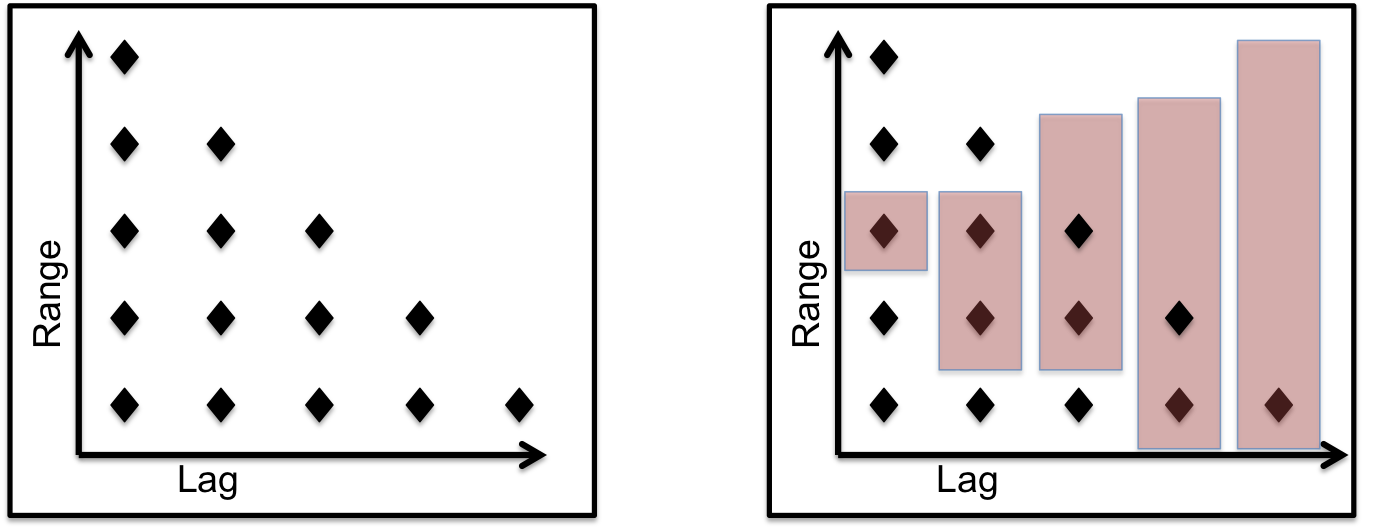
\includegraphics[width=3in]{sumrule}
\caption{Summation Rule Diagram}
\label{fig:sumrule}
\end{figure}

%In the processing this is basically a summing of lags from different ranges. The amount of summing is similar to what is shown in Figure \ref{fig:sumrule}.   



%\begin{equation}
%\label{eq:lagpronoise}
%\hat{R}_w(m,l) = \displaystyle\sum\limits_{j=0}^{J-1} w(m_w-\lfloor l/2\rfloor,j)w^*(m_w+\lceil l/2 \rceil,j),
%\end{equation}

Finally, noise effects are included by subtracting an estimate of the noise correlation from $\widehat{R}_s(m,l)$.  We represent the noise correlation function as $\widehat{R}_w(m,l)$, the ACF estimate of the background noise process of the radar $w(n_w)$ using the steps in Equations \ref{eq:lagpro} and \ref{eq:sumrule}. In a real radar system the noise process is typically sampled either during a calibration period for the radar when nothing is being emitted, or at ranges sufficiently distant that the scattered ionospheric signal is assumed to be negligible. The final estimate of the autocorrelation function after the noise subtraction and summation rule is represented by $\widehat{R}_f(m,l)$.

Along with the first order moment of the ACF seen in Equation \ref{eq:sumruleest}, in order to do error analysis a second order moment is needed. The covariance matrix between each lag estimate can be formed using the formulation in Equation 2 of \cite{hysell2008}, rewritten here as

\begin{equation}
\label{eqn:covcalc}
C_{\tau_1,\tau_2} = \frac{1}{2J} \left( \ R(0)  R^*(\tau_1-\tau_2) +  R(\tau_1) R^*(\tau_2) \right),
\end{equation}

\noindent where, $R(\tau)$ is the estimated ACF as a function of lag $\tau$, $C_{\tau_1,\tau_2}$ is the entry in the covariance matrix of the estimated ACF at lags $\tau_1$ and $\tau_2$,  and $J$ is the number of samples or pulses averaged together to create the estimate. The diagonals of this matrix can be thought of as the autocovariances of each of the lags.  Along these diagonals, by setting $\tau_2 = \tau_1 \equiv \tau$, Equation \ref{eqn:covcalc} simplifies to

\begin{equation}
\label{eqn:covdiag}
C_{\tau,\tau} = \frac{1}{2J} \left(  |R(0)|^2 +|R(\tau)|^2\right).
\end{equation}

The variance of the signal ACF estimate is further increased once sensor and sky noise is added.  If the noise is assumed to be uncorrelated with the signal, the error from the noise, $\left|R_w (\tau)\right|^2$ (e.g. the square of the noise ACF) can be added to the error from the inherent fluctuations in the signal, and the autocovariance expression becomes

\begin{equation}
\label{eqn:covdiagwn}
C_{\tau,\tau} = \frac{1}{2J} \left(  |R(0)|^2 +|R(\tau)|^2 + \left|R_w (0)\right|^2+\left|R_w (\tau)\right|^2\right).
\end{equation}


After the final estimation of the spectrum is complete, nonlinear least squares fitting takes place to determine plasma parameters.  
%\pcom{This entire section can be collapsed to one reference and saved for the thesis chapter.}%
%{
The class of nonlinear least squares problems relevant to ISR parameter estimation can be represented as the minimization of a cost function of the form \cite{kayvol1},

\begin{equation}
	\mathbf{\hat{p}}= \underset{\mathbf{p}}{\text{argmin}} (\mathbf{y}-\bm{\theta}(\mathbf{p}))^*\mathbf{C}_{\mathbf{y}}^{-1}(\mathbf{y}-\bm{\theta}(\mathbf{p})).
\label{nlls}
\end{equation}

In Equation \ref{nlls}, the data represented as $\mathbf{y}$ would be the final estimate of the ACF $\widehat{R}_f(m,l)$ at a specific range, or its spectrum $\widehat{S}_f(m,\omega)$. The matrix $\mathbf{C}_{\mathbf{y}}$  is the covariance matrix from the ACFs or spectra depending on what is being fit. The covariance matrix for the ACF is detailed in Equation \ref{eqn:covcalc}, while the covariance matrix of the spectra is simply the ACF matrix but with discrete Fourier Transforms applied to the rows and columns. The parameter vector $\mathbf{P}$ would be the plasma parameters $N_e$, $T_e$, $T_i$ and $V_i$. The fit function, $\bm{\theta}$, is the IS spectrum calculated from a model mapping these parameters to spectra. For the examples in thesis the model shown in Section~\ref{sec:incohscat}, and in greater detail in Appendix~\ref{appendix1}, is used for this mapping. In order to properly fit the ambiguity function must then be applied to the spectra. In the case of the long pulse the ambiguity can be simply applied by multiplying it with the autocorrelation function $R(l)$ if the summation rule is properly applied. As in previous publications, \cite{nikoukar2008}, the Levenberg-Marquardt algorithm is used to fit the plasma parameters to the ACFs or spectra \cite{levenberg1944,marquardt:1963}.

The Levenberg-Marquardt algorithm moves the parameter vector $\mathbf{p}$ by a perturbation $\mathbf{h}$ at each iteration\cite{gavin:2013}. Specifically Levenberg-Marquart was designed to be a sort of meld between two different methods Gradient Decent, and Gauss-Newton. The perturbation vector $\mathbf{h}_{lm}$ can be calculated using the following:

\begin{equation}
\left[ \mathbf{J}^T\bm{\Sigma}^{-1}\mathbf{J}\right]\mathbf{h}_{lm} =\mathbf{J}^T\bm{\Sigma}^{-1}(\mathbf{y}-\bm{\theta}(\mathbf{p}))
\label{hlm}
\end{equation}

\noindent where $\mathbf{J}$ is the Jacobian matrix $\partial \bm{\theta}/\partial \mathbf{p}$ \cite{levenberg1944,marquardt:1963}. 

The last step is to calculate the errors in the parameter estimates. In order to do this a numerical approximation is computed of the Jacobian matrix between the data and the ACF, $\mathbf{J}$, at $\mathbf{p}=\mathbf{\hat{p}}$. Given this Jacobian, the formula to estimate the parameter error matrix, $\mathbf{C}_{\mathbf{\hat{p}}}$ according to \cite{Hysell:2000cq}, is

\begin{equation}
\label{eqn:jacinv}
\mathbf{C}_{\mathbf{\hat{p}}}=(\mathbf{J}^T \mathbf{C}^{-1}\mathbf{J})^{-1},
\end{equation}
%\begin{equation}
%\label{eqn:jacinv}
%\bm{\Sigma}_{\mathbf{\hat{p}}}=\frac{(\mathbf{J}^T\mathbf{J})^{-1} (\mathbf{y}-\bm{\theta}(\mathbf{\hat{p}}))^*\bm{\Sigma}^{-1}(\mathbf{y}-\bm{\theta}(\mathbf{\hat{p}}))}{L-N_{\mathbf{p}}},
%\end{equation}

\noindent  The variances of the parameters are then taken as the diagonals of the matrix. The off-diagonal elements can be used as a measure of correlation between the different plasma parameters.

%The correlation matrix $\bm{\Sigma}$ is often realized as a diagonal matrix for many ISR systems the variance of the lags or each point of the spectrum being the values. The variance of the ACF estimator can be estimated using the following,
%
%\begin{equation}
%\label{eqn:acfvar}
%\sigma_{\hat{R}(l)}^2=\frac{1}{JL}\displaystyle \sum_{m=-(L-l-1)}^{L-l-1}\left(\frac{L-|m|+1}{L}\right)\left(|\hat{R}(m)|^2 +|\hat{R}(m+l)\hat{R}(m-l)|\right) + \hat{N}^2
%\end{equation}
%
%\noindent where $N$ is the estimated noise power. To estimate the spectrum variance the matrix $\bm{\Sigma}$ is transformed in to the Fourier domain using FFTs (FFT on the columns and IFFT on the rows) so as to model the $\mathbf{F}\bm{\Sigma} \mathbf{F}^*$ matrix operation. 



%%
A simpler formula for estimating the possible uncertainties from ACF is the following:

\begin{equation}
\label{sigpow}
\sigma_i = \frac{S}{\sqrt{J}}\left(1+\frac{1}{SNR}\right).
\end{equation}

\noindent where $S$ is the signal power and $SNR$ is the ratio of signal power to noise power \cite{nicollsisrschool2013}. The noise level can be estimated from the calibration period, which can be done in each IPP after which there is no expected appreciable return from ionosphere incoherent scatter. If there are localized but large returns, for example coherent reflections from satellites, this impact can be reduced by applying estimators that use order statistics \cite{ordstatcfar}.

\section{Summary}
In this Chapter the basic model of ISR and the standard signal processing to perform plasma parameter measurements was examined. The first section detailed the physical intuition and basic model of the IS spectra, essentially how the plasma parameters are mapped to the Doppler spectra. The second section detailed a signal model for a pulsed radar system being used to resolve the IS spectra and compared the model to time-varying filters. Lastly the standard signal processing found in most ISR systems, from sampled complex voltages to estimated plasma parameters, was detailed.
%Using the covariance matrix from the fitted parameters, an overall error estimate can be achieved. This matrix is calculated using a numerical approximation to the Jacobian matrix that the function uses to determine the solution. The Hessian, $\mathbf{H}$ is then calculated by using the Jacobian and then inverted to get the covariance matrix. Due to the way the numerical routines solve the problem, this matrix must be multiplied by the error between the estimated parameters and the data,
%
%\begin{equation}
%\label{eqn:jacinv}
%\bm{\Sigma}_{\mathbf{\hat{p}}}=\frac{(\mathbf{J}^T\mathbf{J})^{-1} (\mathbf{y}-\bm{\theta}(\mathbf{\hat{p}}))^*\bm{\Sigma}^{-1}(\mathbf{y}-\bm{\theta}(\mathbf{\hat{p}}))}{L-N_{\mathbf{p}}},
%\end{equation}

%\noindent where $N_{\mathbf{p}}$ is the number of parameters being fit. The variances of the parameters are then taken as the diagonals of the matrix.}

 %If the Hessian matrix is undefined so it can not be inverted and a proper estimate of the errors is not possible.
 
 
 
 
 
 % from section 2.2
 %With ISR a distribution of electrons are probed, so we have an extremely large number of small cross-section targets within the beam. A better model would be a set of scatterers each with their weighted return and Doppler frequency, represented as
%\begin{equation}
%\label{multiDop}
%\displaystyle x_d(t) = \sum_{n}^{N} x(t)V_ne^{j2\pi f_{n} t}.
%\end{equation}
%This model can be extended to a continuum of signals each with unique Doppler frequency, becoming
%\begin{equation}
%\label{conDop}
%x_d(t) = \int x(t) V(f)e^{j2\pi ft} df.
%\end{equation}
%Pulling the $x(t)$ term out of the integral it is apparent that this is the Fourier transform of this relative weighting between each of the scatterers multiplied with the signal.  This is equivalent to a convolution in frequency space of the spectrum of the original radar signal and the Doppler spectrum with the collection of targets.  
%The final form of the signal spectrum with Doppler added can be shown as the following
%\begin{equation}
%\label{finalDop}
%x_d(t) = \int \left[\int X(\lambda-f)V(\lambda)d\lambda\right] e^{j2\pi f t}df.
%\end{equation}
%This shows that the measured Doppler on the radar signal can be formulated as the convolution of the Fourier transform of the radar signal along with the Doppler spectrum of the target.
%
%This model can be extended from a single point to a much more general form spread across range
%\begin{equation}
%\label{eqn:scateqn}
%x(t)= \int \int V(\mu,f)s(t-\mu)e^{j2\pi f t} d \mu df,
%\end{equation}
%where $V(\mu,\nu)$ is the scatter function and $\mu=2r/c$. One of the earlier uses of this form comes from the study of time varying communication channels \cite{Kailath:1962jx,Kailath:1963gh}. This scattering function drives the methodology on how the target can be properly measured. 
%This model creates two classes of targets, distinguished by range bandwidth product. For the case of an \textit{underspread} target
%\begin{equation}
%\label{eqn:trp}
%B\frac{2r}{c}<1,
%\end{equation}
%where $B$ is the Doppler bandwidth \cite{Pfander:2015ea}. 
%The case of the \textit{overspread} target occurs when this inequality does not hold.



\cleardoublepage

% -------------------------------------
% CHAPTER 3: Space-Time Ambiguity
% -------------------------------------
\chapter{Space-Time Ambiguity Function}
\label{chapter:stamb}
\thispagestyle{myheadings}

% set this to the location of the figures for this chapter. it may
% also want to be ../Figures/2_Body/ or something. make sure that
% it has a trailing directory separator (i.e., '/')!
\graphicspath{{3_STAmb/Figures/}}

%%%%%%%%%%%%%% Intro %%%%%%%%%%%%%%%%%%%%%%%%%%%%%%%%%%%%%
This chapter explains the theoretical backbone for sampling issues associated with ISR. The first section will detail the differences in space-time sampling between single antenna and electronically steerable array (ESA) systems. The next section will then detail the derivation of the space-time ambiguity. Lastly the impact of moving plasma on the apparent ambiguity will be shown, both from a theoretical stand point and a demonstration using collected ISR data.


\section{Space-Time Sampling}
\label{sec:sptimesamp}
These new ESA based systems differentiate themselves from dish antennas in a fundamental way. Instead of dwelling in a single beam or scanning along a prescribed direction, an ESA can move to a different beam position within its field of view on a rapid, pulse by pulse basis. An illustration of the differences between ESA and conventional radar systems with respect to statistical integration of radar pulses, focusing on time history of beam positions, starts with the desired grid of geographic parameter coverage in Figure \ref{fig:bp1}. Figure \ref{fig:dbsts} shows a possible path for a dish based antenna to cover this measurement space through moves to different beam positions through time, represented on the z-axis as pulse repetition intervals (PRIs). The dish sweeps through the field of view in a continuous scan.  In contrast, an ESA system can instead move from position to position in discrete steps as seen in Figure \ref{fig:phbsts}. It is noted as well that the phased array antenna is able to collect data from different beams during overlapping time periods, creating a lattice like pattern. This type of pulse-to-pulse beam position change is very difficult to accomplish with dish antenna systems having significant pointing inertia. 

\begin{figure}
	\centering
	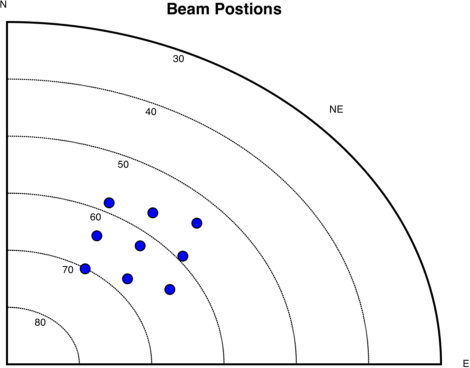
\includegraphics[width=3.5in]{beampositionssts}
	\caption{A 3x3 grid of desired measurement positions in a
         hypothetical geodetic latitude/longitude space. }
	\label{fig:bp1}
\end{figure}

\begin{figure}
	\centering
	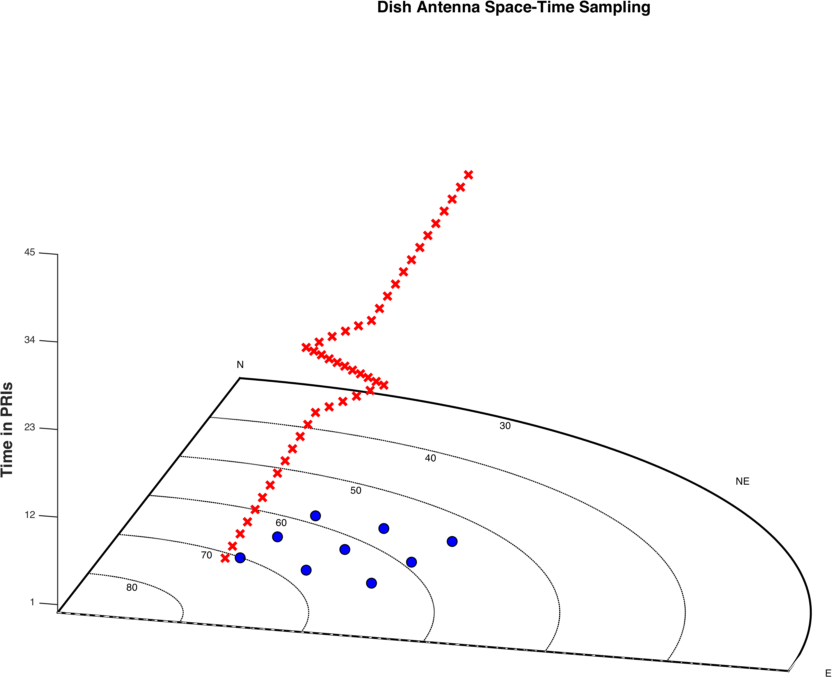
\includegraphics[width=3.5in]{dishsts}
	\caption{Space-time sampling of the measurement space from Figure~\ref{fig:bp1} using a dish based antenna, where the red x's mark the pulse in beam space and time. Beam positions from Figure \ref{fig:bp1} are shown below in blue at $z=0$.}	
	\label{fig:dbsts}
\end{figure}

\begin{figure}
	\centering
	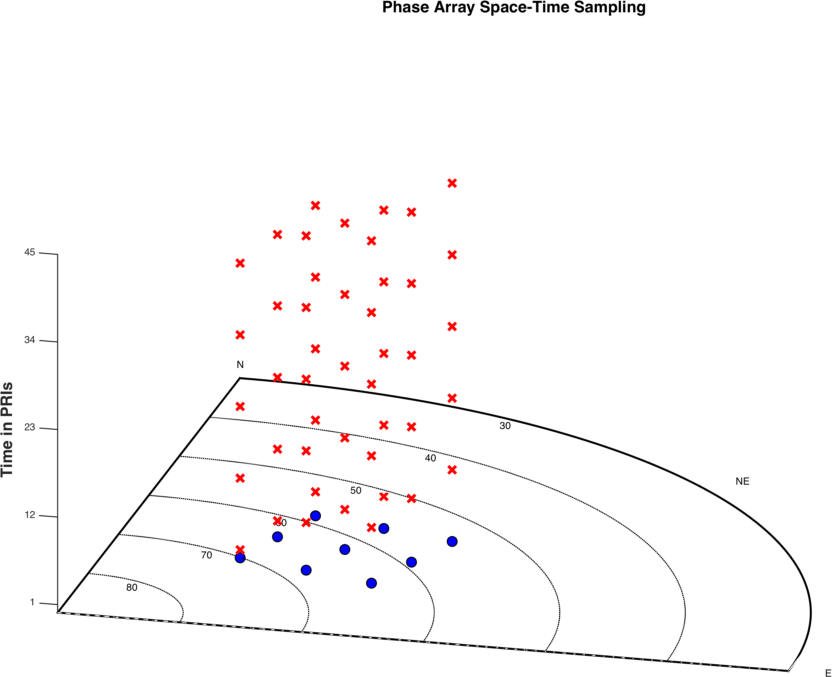
\includegraphics[width=3.5in]{phasedarraysts}
	\caption{Space-time sampling of the measurement space from Figure~\ref{fig:bp1} using a phased array based antenna, where the red x's mark the pulse in beam space and time. Beam positions from Figure \ref{fig:bp1} are shown below in blue at $z=0$.}	
	\label{fig:phbsts}
\end{figure}

The rapid steering ability of ESA systems relative to space-time sampling yields a new flexibility, in post processing, to statistically combine information from different beams using knowledge of the plasma velocity field, where this information is obtained either from external sources or from the Doppler shift of the ionospheric echoes themselves. This can help to relax the assumption of stationarity for plasmas that are evolving or changing their shape on time scales longer than the integration time. If the plasma moves into a different beam, returns from the same plasma can be integrated together with proper bookkeeping. This is contrary to the situation with dish antennas where returns from multiple plasma populations with different parameter sets are unavoidably averaged together.


\section{Space-Time Ambiguity}
\label{sec:sptimeamb}

The space-time ambiguity can be thought of as a kernel to a combined volume and time integration operator. In the derivations that follow, it is shown that this ambiguity can be represented as a kernel operator in a Fredholm integral equation:

\begin{equation}
\label{eqn:friedholm}
\rho(\tau_s ,\mathbf{r}_{s},t_s) = \int L(\tau_s, \mathbf{r}_{s},t_s,\tau,\mathbf{r},t) R(\tau,\mathbf{r},t) dVd t d\tau
\end{equation}

\noindent where, for ISR, $L(\tau_s, \mathbf{r}_{s},t_s,\tau,\mathbf{r},t) $ is a blurring kernel over time and space, and $R(\tau,\mathbf{r},t) $ indicates the plasma medium's autocorrelation function at the lag $\tau$, time $t$, and position $\mathbf{r}$.

By using this formulation, many parallels between ISR and classic camera blurring problems can be made. In cameras, blurring can take place when an object moves over a space covered by one pixel while the shutter is open and the CCD is collecting photons. A diagram of this can be seen in Figure \ref{fig:ccd}. The same holds for the ISR measurement problem, except that the pixels are no longer square or continuous in Cartesian space and instead are determined by the beam shape and pulse pattern. This is shown in the diagrams in Figure \ref{fig:radarblur}.


\begin{figure}[h!]
\centering
	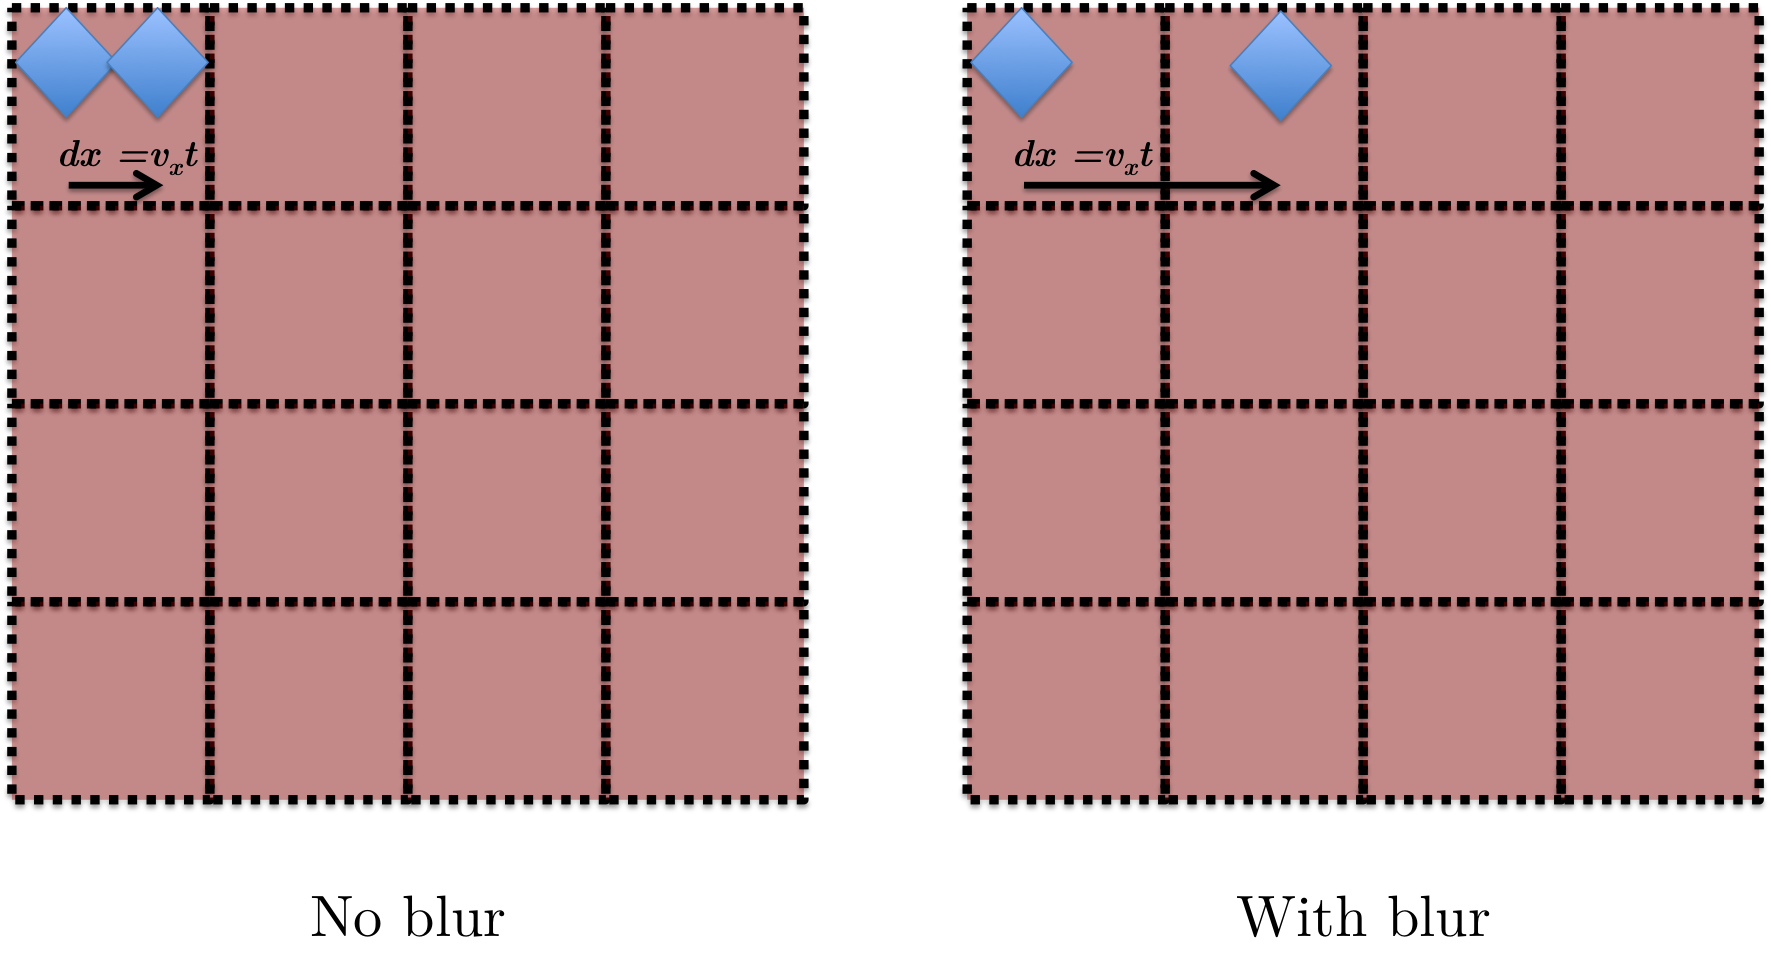
\includegraphics[width=4in]{ccddiagramall}
	\caption{CCD resolution cell diagram, showing cases where an object will be properly resolved and be blurred.}
	\label{fig:ccd}
\end{figure}

\begin{figure}[h!]
\centering
	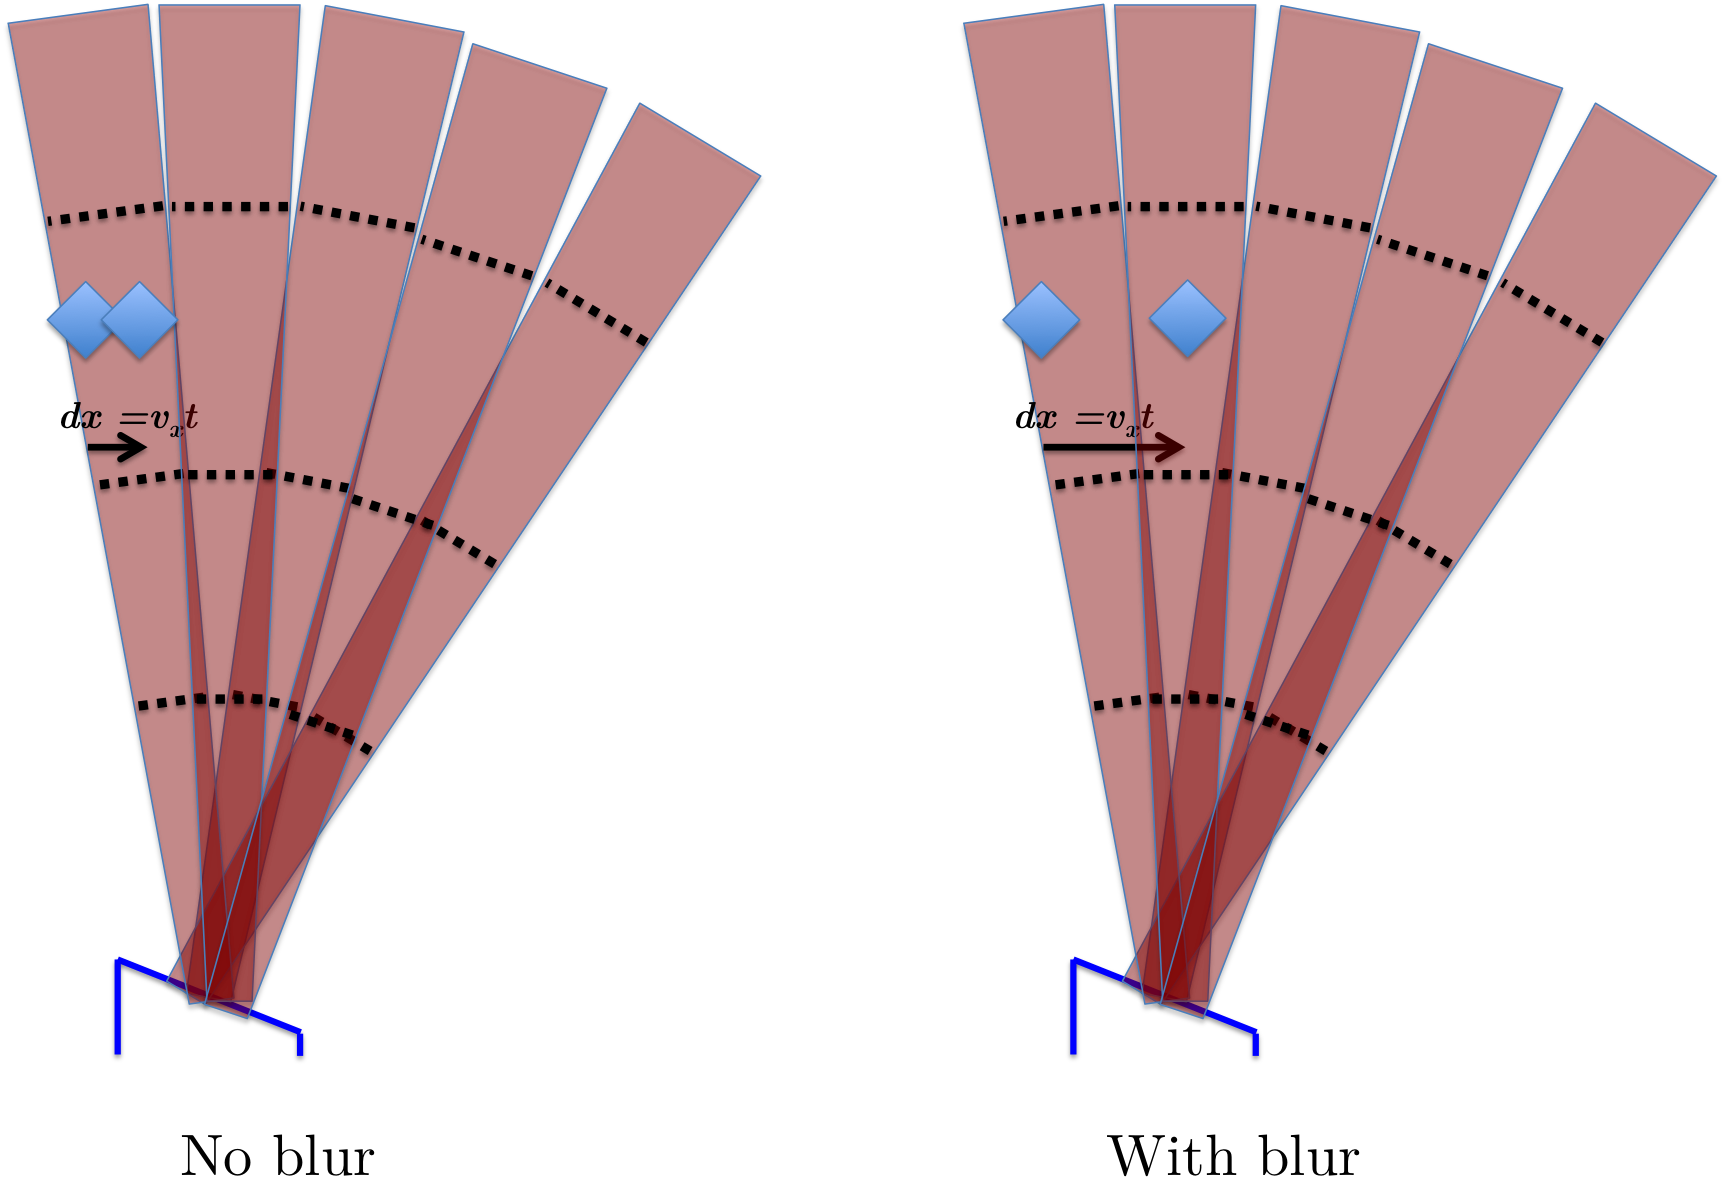
\includegraphics[width=4in]{radardiagramall}
	\caption{ISR resolution cell diagram, showing cases where an object will be properly resolved and be blurred.}
	\label{fig:radarblur}
\end{figure}

\subsubsection{Coordinate System Definitions}

Before the full space-time ambiguity function, $L(\tau_s,\mathbf{r}_s,t_s,\tau,\mathbf{r},t)$, derivation starts the coordinate system will be defined.  The three dimensional coordinate system is defined as $\mathbf{r}=[x,y,z]^T$. For this coordinate system, $\mathbf{r}=[0,0,0]^T$ at the location of the radar and thus $r=|\mathbf{r}|$, also known as the range variable. This allows for the use of polar coordinates $\mathbf{r} =  [r,\theta_,\phi]^T$ where $\theta$ and $\phi$ are, respectively, the observer's elevation and azimuth angles.

The radar samples this space at a set of discrete points which will be referred to as $\mathbf{r}_s = [x_s,y_s,z_s]^T$ along with the discretized range expression $r_s=|\mathbf{r}_s|$. The sampled space consists of a number of points, composed of range gates within a beam multiplied by the number of beams. These points can also be referred in polar coordinates $\mathbf{r}_s = [r_s,\theta_s,\phi_s]^T$, where $\theta_s$  and $\phi_s$ are, respectively, the observationally sampled elevation and azimuth angles.

For notation purposes, two different sets of time are used, commonly known in the hard-target radar literature as fast-time, $n$ and slow-time, $t$ \cite{richards:fundamentalsigproc}. Fast-time is used to describe processes with correlation time less than one PRI. Slow-time will be used for processes that decorrelate in time on the order of, or longer than, the system's PRI. In order to form estimates of ACFs with desired statistical properties, it is assumed that the plasma parameters parameters will change on the order of many tens to hundreds of PRIs in their stationary reference frame (i.e. remain wide sense stationary for this time). Generally, for incoherent scatter applications in the E-region of the ionosphere ($\approx$100 km altitude) and above, the decorrelation time is less than a PRI for systems with a center frequency in the UHF band, and thus ACFs must be formed over fast-time.

The terms $n$ and $t$ represent continuous variables, while $n_s$ and $t_s$ will be the fast time and slow time parameters sampled by the radar. The sampling rate of $n_s$ is set by the rate at which the system's A/D converters are run. The sampling of $t_s$ can, at the highest rate, be the PRI. At its lowest rate, it can be sampled once in a non-coherent processing interval (NCPI), or equivalently in a period of time it takes the radar to average the desired number of pulses for each beam. 

\subsubsection{Derivation}

The physical scattering mechanism underlying ISR produces measurable radar scatter from electron density fluctuations in the ionosphere, $n_e(\mathbf{r},n)$, at a specific wavenumber $\mathbf{k}$. These fluctuations scatter radio waves which can be observed by the receiver system of the radar \cite{dougherty:farley1960}. The emitted radar signal at the transmitter has a pulse shape $s(n)$ modulated at a central frequency creating a scattering wave number $\mathbf{k}$. Using the Born approximation, the signal received at time $n$, $x(n)$, can be represented as the following

\begin{equation}
\label{eq:xt}
x(n) = h(n) \ast \int \exp\left[-j\mathbf{k} \cdot \mathbf{r}\right]  s\left(n-\frac{2r}{c}\right) n_e(\mathbf{r},n) d\mathbf{r},
\end{equation}

\noindent where $h(n)$ is the receiver filter and the $\ast$ represents the convolution operator. In modern ISR systems, this signal $x(n)$ is then sampled at discrete points in fast-time which will be referred to as $n_s$. The convolution and sampling operation can be brought in the integral as the following,

\begin{equation}
\label{ex:xtaug}
x(n_s) = \int \exp\left[-j\mathbf{k} \cdot \mathbf{r}\right]  s\left(n-\frac{2r}{c}\right) n_e(\mathbf{r},n)h(n_s-n) d\mathbf{r}dn
\end{equation}


Once the signal has been received and sampled, the autocorrelation function is then estimated from the sampled signal $x(n_s)$. The full expression of the underlying autocorrelation of this signal is the following, 

\begin{multline}
\label{ex:acf0}
\langle x(n_s)x^*(n_s')\rangle =  \int \exp\left[-j \mathbf{k}\cdot \left(\mathbf{r}'-\mathbf{r} \right)\right]s\left(n-\frac{2r}{c}\right)s^*\left(n'-\frac{2r'}{c}\right) \\ h(n_s-n)h(n_s'-n')\langle n_e(\mathbf{r},n)n^*_e(\mathbf{r}',n')\rangle d\mathbf{r} d\mathbf{r}'dn dn',
\end{multline}

\noindent where $r'$ is the magnitude of the vector $\mathbf{r}'$. By assuming stationarity of second order signal statistics along fast time, lag variables $\tau\equiv n'-n$, and $\tau_s\equiv n_s'-n_s$ can be substituted. With these substitutions, Equation \ref{ex:acf0} becomes


\begin{multline}
\label{ex:acf1}
\langle x(n_s)x^*(n_s+\tau_s)\rangle =\int \exp\left[-j \mathbf{k}\cdot \left(\mathbf{r}'-\mathbf{r} \right)\right]s\left(n-\frac{2r}{c}\right)s^*\left(n+\tau-\frac{2r'}{c}\right) \\ h(n_s-n)h(n_s+\tau_s-n-\tau) \langle n_e(\mathbf{r},n)n^*_e(\mathbf{r}',n+\tau)\rangle d\mathbf{r} d\mathbf{r}' dnd\tau
\end{multline}

\noindent A simplifying assumption at this point that the space-time autocorrelation function of $n_e(\mathbf{r},t)$, $\langle n_e(\mathbf{r},n)n_e(\mathbf{r}',n+\tau)\rangle$, will go to zero as the magnitude of $\mathbf{y} \equiv \mathbf{r}'-\mathbf{r}$ increases beyond the Debye length \cite{farley1969}. Thus, the rate which the spatial autocorrelation goes to zero will be such that $\tau\gg \frac{2||\mathbf{y}||}{c}$, allowing us to set $r= r'$ inside the arguments of $s$ and $h$. This allows Equation \ref{ex:acf1} to be rewritten as 
 
 \begin{multline}
 \label{ex:acf2}
 \langle x(n_s)x^*(n_s+\tau)\rangle = \int s\left(n-\frac{2r}{c}\right)s^*\left(n+\tau -\frac{2r}{c}\right) h(n_s-n)h^*(n_s+\tau_s-n-\tau) \\\left[\int \exp\left[-2j \mathbf{k}\cdot \mathbf{y}\right] \langle n_e(\mathbf{r},n)n^*_e(\mathbf{y}+\mathbf{r},n+\tau)\rangle d\mathbf{y} \right]drdn d\tau.
 \end{multline}

The inner integral is a spatial Fourier transform evaluated at the Bragg vector of radar $\mathbf{k}$. By again asserting stationarity along fast time, the true ACF can be represented as the following,
 \begin{equation}
 \label{eq:spft}
R(\tau,\mathbf{r})= \langle |n_e(\mathbf{k},r,\tau)|^2\rangle \equiv  \int \exp\left[-2j \mathbf{k}\cdot \mathbf{y} \right] \langle n_e(\mathbf{r},b)n^*_e(\mathbf{y}+\mathbf{r},n+\tau)\rangle d\mathbf{y}.
 \end{equation}
 
 \noindent Now Equation \ref{ex:acf2} becomes
 
 \begin{equation}
 \label{eqn:inbetween}
 \begin{split}
 \langle x(n_s)x^*(n_s+\tau_s)\rangle =& \int \langle |n_e(\tau,\mathbf{k},\mathbf{r})|^2\rangle \times\\ &\left[\int s(n-\frac{2r}{c})s^*(n+\tau -\frac{2r}{c})h(n_s-n)h^*(n_s+\tau_s-n-\tau) dn \right]d\tau dr.
 \end{split}
 \end{equation}

 If $n_s$ is replaced with $2r_s/c$ we can introduce the range ambiguity function $W(\tau_s,r_s,\tau,r)$ by doing the following substitution,
 \begin{equation}
 \label{eqn:rngamb}
 W(\tau_s,r_s,\tau,r)= \int s(n-\frac{2r}{c})s^*(n+\tau -\frac{2r}{c})h(2r_s/c-n)h^*(2r_s/c+\tau_s-n-\tau) dn.
 \end{equation}
 
Assuming, for the moment, that $R(\tau,\mathbf{r})$ only varies across the range dimension $r$, this can be represented in the form of a Fredholm integral equation
 
 \begin{equation}
 \label{eqn:fredfirst}
 \langle x(2r_s/c)x^*(2r_s/c+\tau_s)\rangle = \int W(\tau_s,r_s,\tau,r)R(\tau,r) drd\tau.
 \end{equation}
 
\noindent The range ambiguity function, $W(\tau_s,r_s,\tau,r)$, can be thought of as a smoothing operator along the range and lag dimensions of $R(\tau,r)$. This result is also derived in \cite{nikoukar2008}, \cite{Woodman:1991is} and \cite{hysell2008}

 
The spatial ambiguity across azimuth and elevation angles is determined by the antenna beam pattern. In phased array antennas, this beam pattern is ideally the array factor multiplied by the element pattern \cite{Balanis:2005:ATA:1208379}. The array factor is determined by a number of things including the element spacing and the wave number of the radar, $k$. For example, by making idealized assumptions with no mutual coupling and that the array elements are simple cross dipole elements, AMISR systems will have the following antenna pattern for pointing angle ($\theta_s,\phi_s$): 

 \begin{equation}
 \label{eqn:amisrpat}
F(\theta_s,\phi_s,\theta,\phi) = \frac{1}{2}(1+\cos(\theta)^2)\left[ \frac{1}{MN} \left(1+\exp\left[j(\psi_y/2 + \psi_x)\right]\right)\frac{\sin((M/2) \psi_x)}{\sin(\psi_x)} \frac{\sin((N/2) \psi_x)}{\sin(\psi_x/2)}\right]^2,
 \end{equation}
 
 \noindent where $\psi_x = -k d_x(\sin\theta\cos\phi-\sin\theta_s\cos\phi_s)$, $\psi_y = -k d_y(\sin\theta\sin\phi-\sin\theta_s\sin\phi_s)$ and $M$ is the number of elements in the $x$ direction of the array, and $N$ is the number of elements in the $y$ direction(see Appendix: \ref{App:AMISRarr} for derivation).


The spatial ambiguity is a separable function made up of the components of $W(\tau_s,\tau,r_s,r)$ and $F(\theta_s,\phi_s,\theta,\phi)$. These two functions can be combined by multiplying the two, creating the spatial ambiguity function  $K(\tau_s,\mathbf{r}_s,\tau,\mathbf{r})$. This yields an expression for a single statistical realization of the ACF of the incoherent scatter random process, which will be referred to as $\rho(\tau_s,\mathbf{r}_s)$:


 \begin{align}
  \label{eqn:volume}
\rho(\tau_s,\mathbf{r}_s) &= \int F(\theta_s,\phi_s,\theta,\phi)W(\tau_s,r_s,\tau,r) R(\tau,\mathbf{r}) dV d\tau ,\\
	&= \int K(\tau_s,\mathbf{r}_s,\tau,\mathbf{r}) R(\tau,\mathbf{r})  dVd\tau.
\end{align}

A rendering of an example of this full spatial ambiguity function for an uncoded long pulse, with antenna pattern from Equation \ref{eqn:amisrpat} for four beams, can be seen in Figure \ref{fig:amb4}.

\begin{figure}
	\centering
	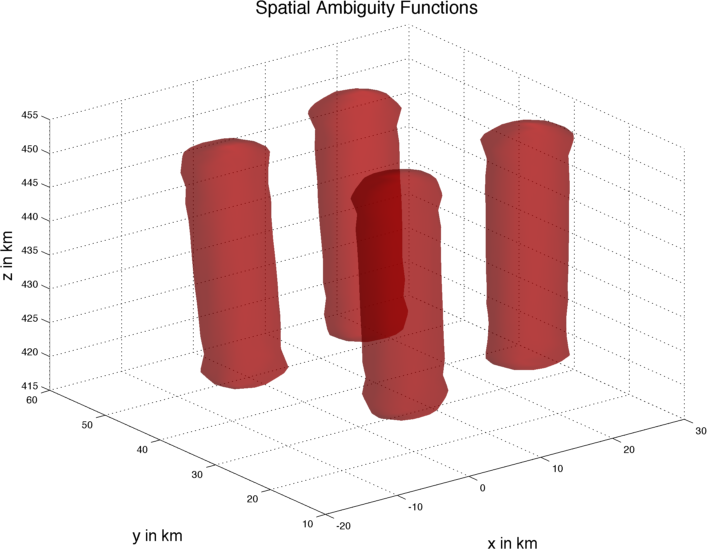
\includegraphics[width=4in]{spaceamb}
	\caption{Full spatial ambiguity function in Cartesian space for case with 4 beams with trailing edge of a 240$\mu$s pulse at 400km range. The surface represents the half power point of the ambiguity function.}	
	\label{fig:amb4}
\end{figure}

As mentioned above, this one pulse ACF estimate represents a single sample of a random process. In order to create a usable estimate, multiple samples of this ACF need to be averaged together to reduce the variance to sufficient levels in order to fit the estimate to a theoretical ACF that is a direct function of plasma parameter values. To show the impact of this averaging in creating the estimate of the ACF, a slow-time dependence will be added to the expression for the medium ACF, which now becomes $R(\tau,\mathbf{r},t)$, and will also add another separable function $G(t_s,t)$ to the kernel. This function $G(t_s,t)$ can be thought of as a sampling and blurring kernel for the ACF if the plasma parameters change within an NCPI. Since the amount of time that the radar pulse is illuminating the plasma in a point of space is very short compared to the PRI, $G(t_s,t)$ can take the form of a summation of Dirac delta functions 

\begin{equation}
\label{eqn:Gexp}
G(t_s,t) = \displaystyle \sum_{j=0}^{J-1}\alpha_j \delta(t-t_s-jT_{REV}),
\end{equation}

\noindent where $J$ counts the number of pulses used over a NCPI, $T_{REV}$ is the amount of time it takes the radar to revisit the specific beam and $\alpha_j$ represent the weights that the radar assigns to the pulses. For systems using pulse-to-pulse steering, one strategy revisits each beam sequentially, in this case making $T_{REV}=N_{beam}T_{PRI}$, where $N_{beam}$ is the number of beams and $T_{PRI}$ is the PRI time period. For the case where weights are set to $1/J$, this operation simply averages the pulses. With Equation \ref{eqn:Gexp} incorporated into the overall ambiguity we obtain the full integral equation,

\begin{equation}
\label{eqn:sptamb}
	\rho(\tau_s,\mathbf{r}_s,t_s) =\int L(\tau_s,\mathbf{r}_s,t_s,\tau,\mathbf{r},t)R(\tau,\mathbf{r},t)dVdtd\tau.
\end{equation}

\noindent The final kernel, $L(\tau_s,\mathbf{r}_s,t_s,\tau,\mathbf{r},t) = G(t_s,t)K(\tau_s,\mathbf{r}_s,\tau,\mathbf{r})$, encompasses the full space-time ambiguity.

\section{Ambiguity after Frame Transformation}
\label{sec:frametrans}

This section will focus on the impact of the motion of plasma as it is going through the field of view of the radar. It will be assumed that the radar is integrating over a length of time $T$ beginning at $t_s$. The kernel $L$ will be represented as a separable function $K$ and $G$ as in Equation \ref{eqn:sptamb}. In this case, $G$ will be a summation of Dirac delta functions with weights of $1/J$. This will change Equation \ref{eqn:sptamb} to the following:

\begin{equation}
\label{eqn:L2}
\rho(\tau_s,\mathbf{r}_s,t_s) = \int K(\tau_s,\mathbf{r}_s,\tau,\mathbf{r}) \left[(1/J)\int_{t_s}^{t_s+T} \displaystyle \sum_{j=0}^{J-1} \delta(t-t_s-jT_{REV})R(\tau,\mathbf{r},t) dt\right] dVd\tau.
\end{equation}

Of specific interest in this study are instances in the high latitude ionosphere where embedded plasma structures are moving due to electric field drivers applied by the magnetosphere. In this case, it will be assumed that the plasma is a rigid object and will not deform with respect to $\mathbf{r}$ over time period $[t_0,t_0+T]$ where $T=JT_{REV}$ is the time for one NCPI. Also, it will be assumed that the plasma parcel moves with a constant velocity $\mathbf{v}$. Thus $R(\tau,\mathbf{r},t)\Rightarrow R(\tau,\mathbf{r}+\mathbf{v}t)$. The assumption of rigidity can in some cases be valid over the time period of the NCPI, on the order of a few minutes, while the plasma moves through the field of view of the radar. For example, in the high latitude ionosphere, large scale features in structures such as patches decay on the order of hours \cite{Tsunoda:1988ul}. This assumption is useful because it allows our framework to analyze impacts of these plasma variations on the parameter resolution of ISR systems. With these assumptions, Equation \ref{eqn:L2} becomes,

\begin{equation}
\label{eqn:L3}
\rho(\tau_s,\mathbf{r}_s,t_s) =(1/J) \int \int_{t_s}^{t_s+T} \displaystyle \sum_{j=0}^{J-1}\delta(t-t_s-jT_{REV}) K(\tau_s,\mathbf{r}_s,\tau,\mathbf{r})R(\tau,\mathbf{r}+\mathbf{v}t)dtdVd\tau\end{equation}

A change of variables to $\mathbf{r}' = \mathbf{r}+\mathbf{v}t$ acts as a Galilean transform and applies a warping to the kernel, changing the frame of reference. Since $R(\tau,\mathbf{r}')$ is no longer dependent on $t$, Equation \ref{eqn:L3} can be integrated in time and becomes:

\begin{equation}
\label{eqn:L5}
\rho(\tau_s,\mathbf{r}_s,t_s)= (1/J)\int \left[ \;\;  \displaystyle \sum_{j=0}^{J-1} K(\tau_s,\mathbf{r}_s,\tau,\mathbf{r}'-\mathbf{v}(t_s+jT_{REV})) \;\; \right]R(\tau,\mathbf{r}')dVd\tau.
\end{equation}

The problem can now be simplified further back to a Fredholm integral equation by simply replacing the terms in the square brackets as a new kernel $A(\tau_s,\mathbf{r}_s,t_s,\tau,\mathbf{r}')$:

\begin{equation}
\label{eqn:L6}
\rho(\tau_s,\mathbf{r}_s,t_s)= \int A(\tau_s,\mathbf{r}_s,t_s,\tau,\mathbf{r}') R(\tau,\mathbf{r}')dVd\tau.
\end{equation}

\noindent The impact of the plasma velocity on the ambiguity function can be seen in Figure \ref{fig:ambtime}. This is the same ambiguity as seen in Figure \ref{fig:amb4} but with a velocity of 500 m/s in the $y$ direction over a period of 2 minutes. This velocity creates a larger ambiguity function in the frame of reference of the moving plasma.

\begin{figure}[!t]
	\centering
	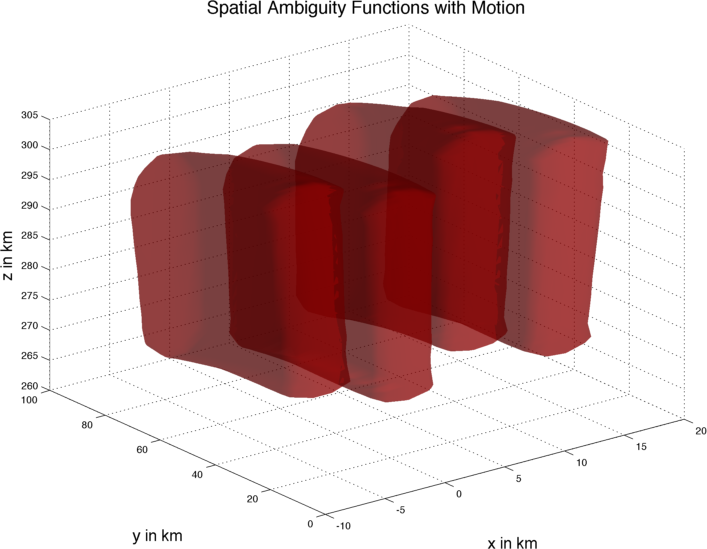
\includegraphics[width=4in]{spaceambmoving}
	\caption{Same spatial ambiguity as in Figure \ref{fig:amb4} but now with 500 m/s velocity in $y$ direction in plasma frame of reference. The surface represents the half power point of the ambiguity function.}
	\label{fig:ambtime}
\end{figure}

The operator $A$ can be determined through knowledge of the radar system's beam pattern along with the experiment's pulse pattern, integration time and inherent velocity of the plasma. This velocity $\mathbf{v}$ could be separately estimated by taking measurements of the Doppler shift by using a methodology like that seen in \cite{butler:imagingfregiondrifts}. With this strategy, the operator is now acting purely as a spatial blurring function instead of a full space-time function. It is noted that reducing dimensionality of the problem can make it easier to solve the inverse problem in practice.

\section{Example of Impact on Real ISR Data}

With knowledge of the ambiguity the possible size of features can be inferred. An example using real data can further elucidate this idea. One way that the true size of features is comparing real data with possible inputs and applying the ambiguity to them. Often, researchers using ISR combine data from different sensors \cite{Dahlgren:2012dq}, such as all sky camera data \cite{Shiokawa1999,GRL:GRL21871,Shiokawa2009}. This combination of information allows for researchers to get a better understanding of the underlying physical phenomena.

An example of real data that shows how features could have been impacted by this ambiguity is seen through the series of images in Figure \ref{fig:realdataplane3points}. The auroral arc, seen as an electron density enhancement in the radar data and a brightness enhancement in the optical data, is moving along horizontal position of the plane over a two minute integration period for each image. The radar data is sampled in a spherical coordinate space, thus it is necessary to use some sort of interpolation to view it on the plane of motion, in this case natural neighbors. 

\begin{figure}[h!]
	\centering
	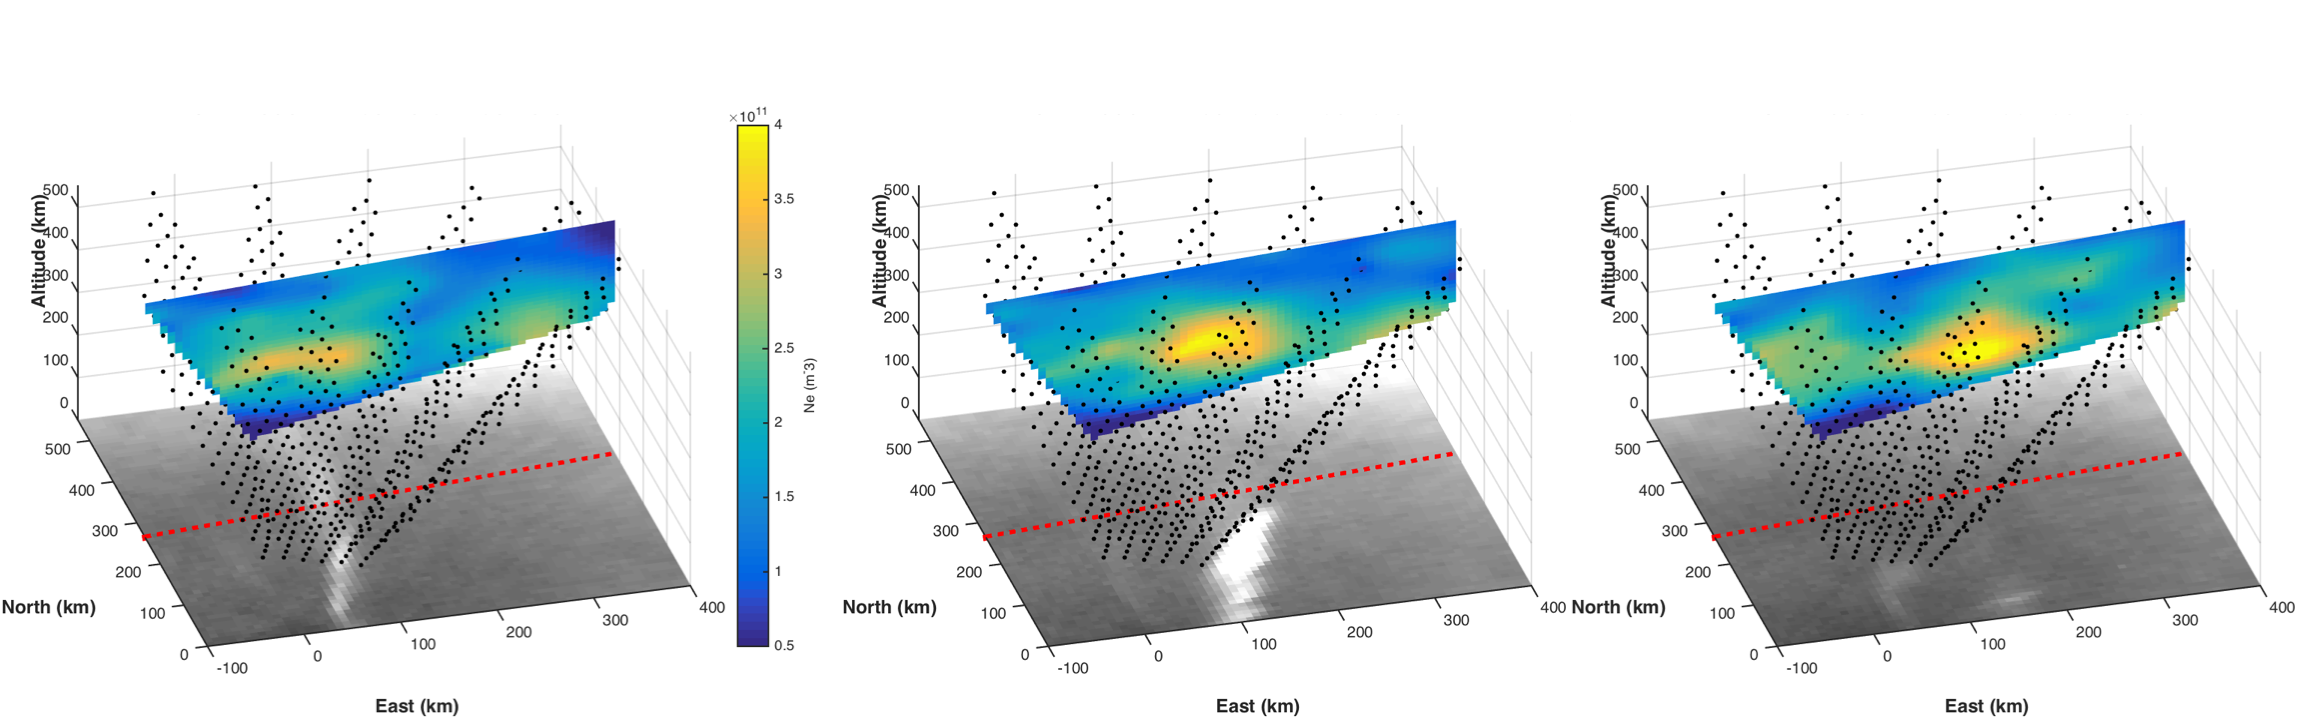
\includegraphics[width=6in]{radarwithoptical}
	\caption{Data taken from the Resolute Bay Incoherent Scatter Radar (RISR) and interpolated along the plane of motion of the auroral arc with green line emission optical data plotted underneath. Each image is a plotted over a two minute integration time for the radar. Also in the image is the sample points of the radar (black dots) and the path of the auroral emission. }
	\label{fig:realdataplane3points}
\end{figure}

The final set of radar data seen in Figure \ref{fig:realdataplane3points} is replotted in Figure \ref{fig:realdataplane} without other data sets and sampling grids. This will help with the comparisons to the following figures, which are plotted along the same plane of motion.

\begin{figure}[h!]
	\centering
	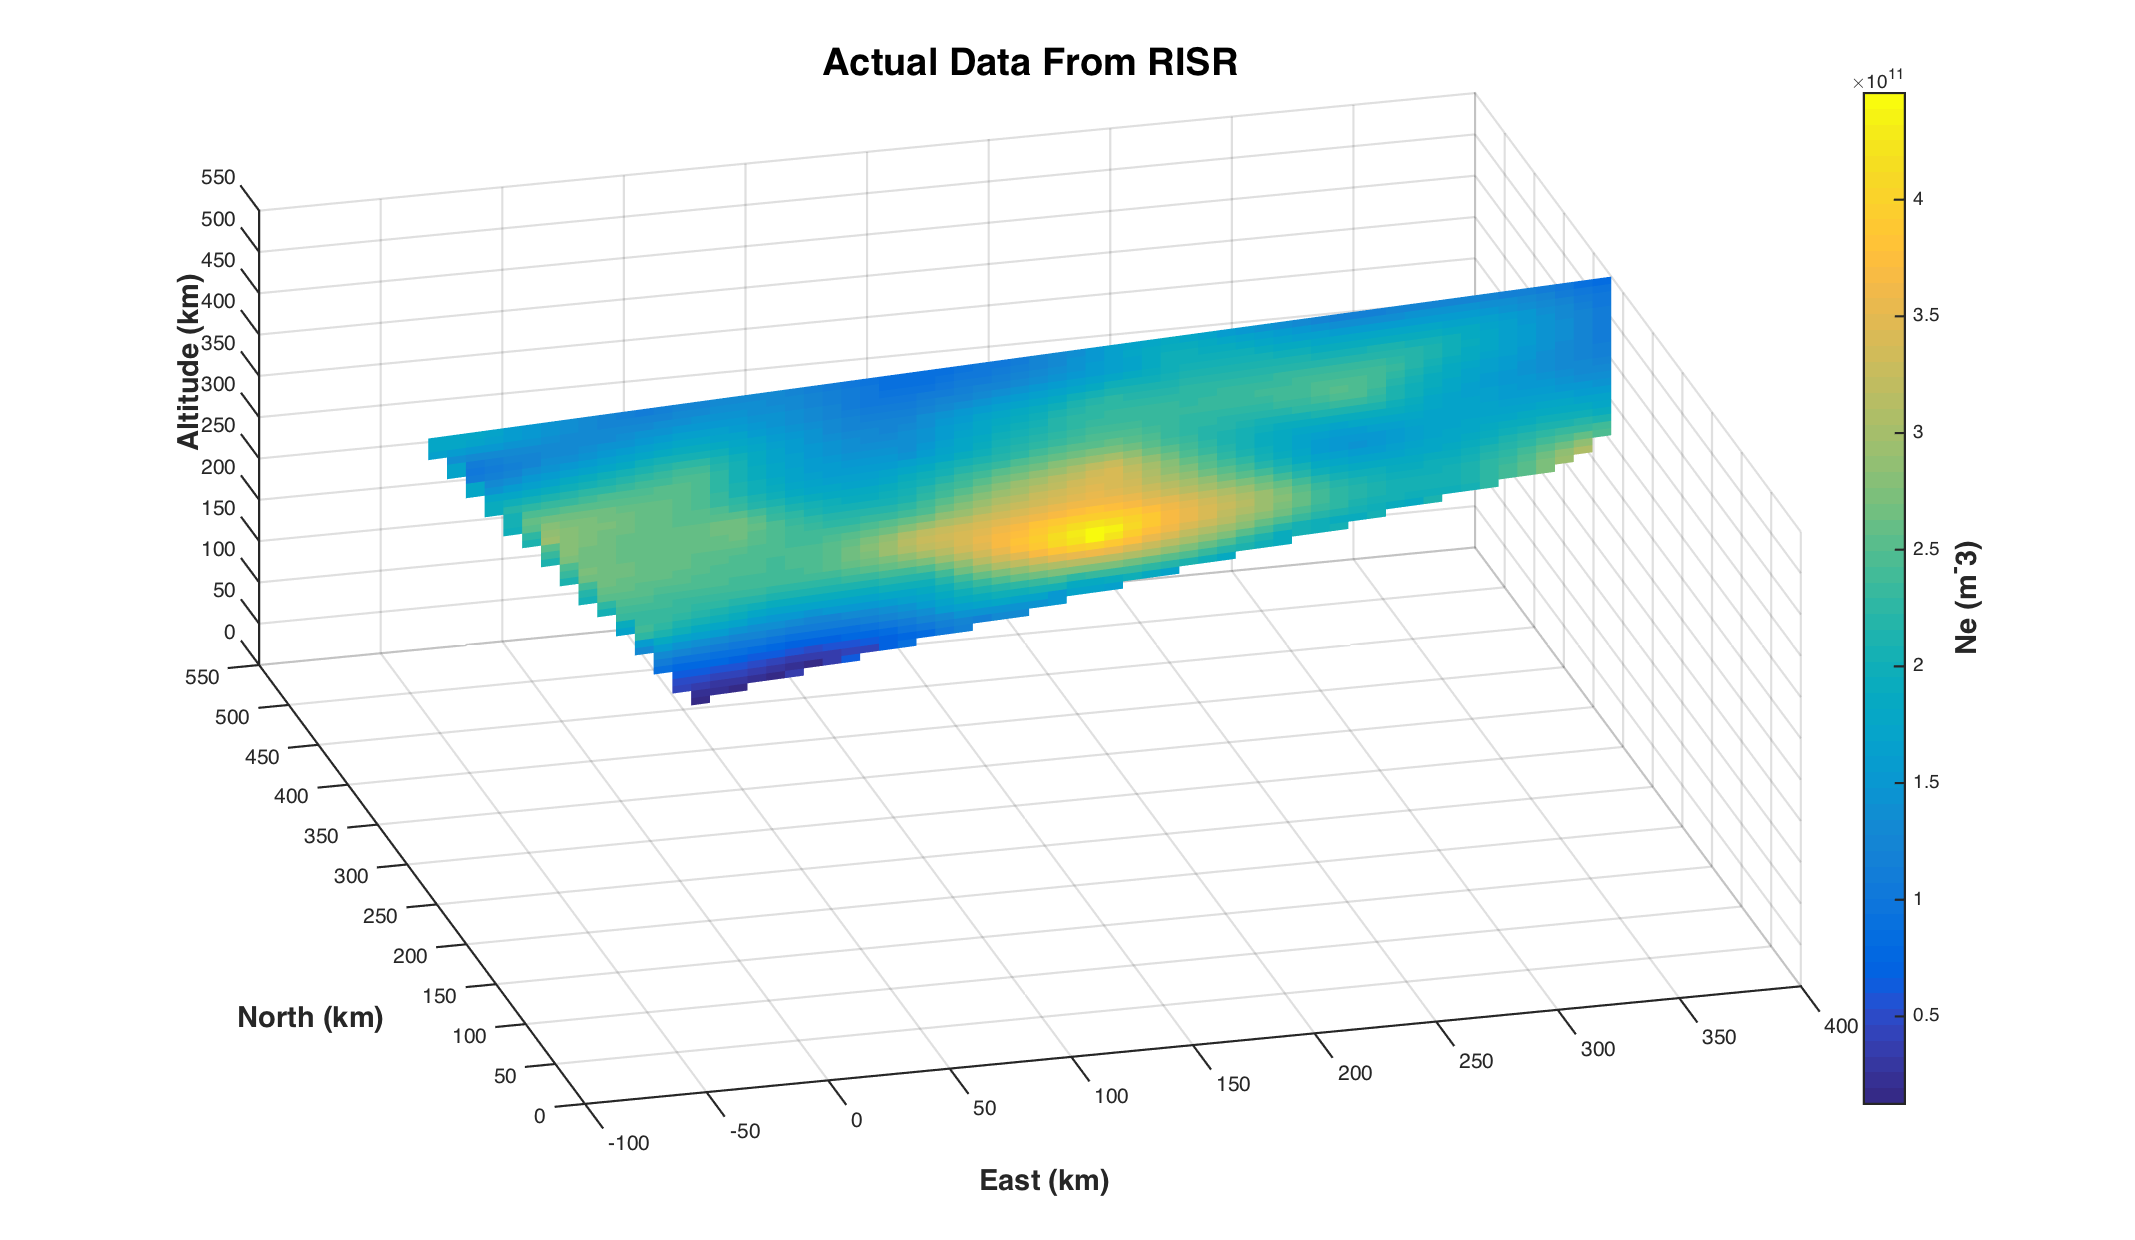
\includegraphics[width=3.5in]{acdata}
	\caption{Data taken from the Resolute Bay Incoherent Scatter Radar (RISR) and interpolated along the plane of motion of the auroral arc.}
	\label{fig:realdataplane}
\end{figure}

The specific experiment beam pattern yielded a sampling pattern seen as the black dots in \ref{fig:rambplane}. The specific result of the ambiguity along the the plane of the motion can give a basic idea of the "resolution" of the image of the objects if there is not motion. Also, it can show if an object may be hidden if stationary during the integration time.

\begin{figure}[h!]
	\centering
	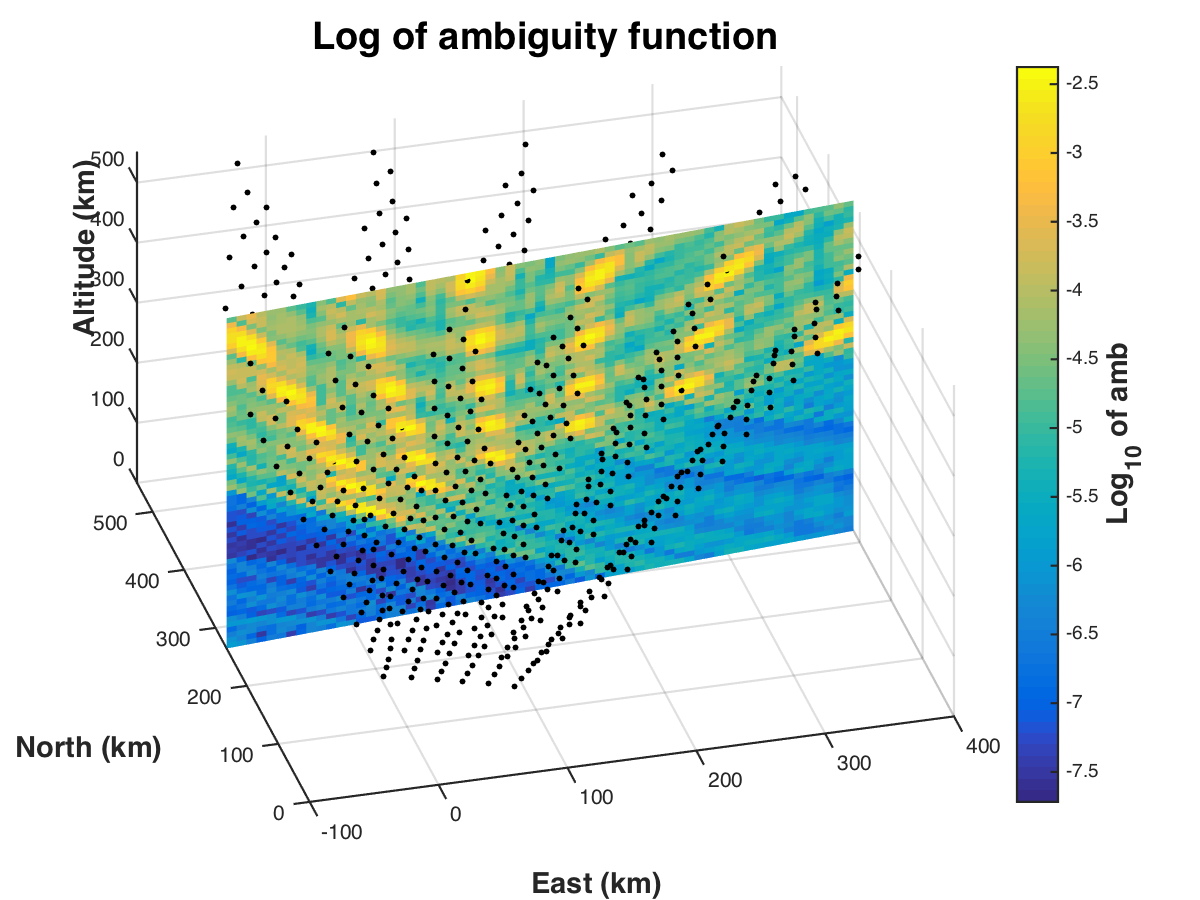
\includegraphics[width=3.5in]{ambplane}
	\caption{The three dimensional sampling pattern as black dots and spatial ambiguity plotted on to along the plane of motion along the auroral arc.}
	\label{fig:rambplane}
\end{figure}

In order to find the actual size of the feature in Figure \ref{fig:realdataplane} we have to take into account the ambiguity in Figure \ref{fig:rambplane} along with any motion that may be present in the feature. The feature shown in Figure \ref{fig:simdataplaneorig} is a possible distribution that could create a similar measurement seen in Figure  \ref{fig:realdataplane}. Using the optical data we have inferred that that this feature is from a cylinder with a Gaussian shaped cross-sectional plasma density. 

\begin{figure}[h!]
	\centering
	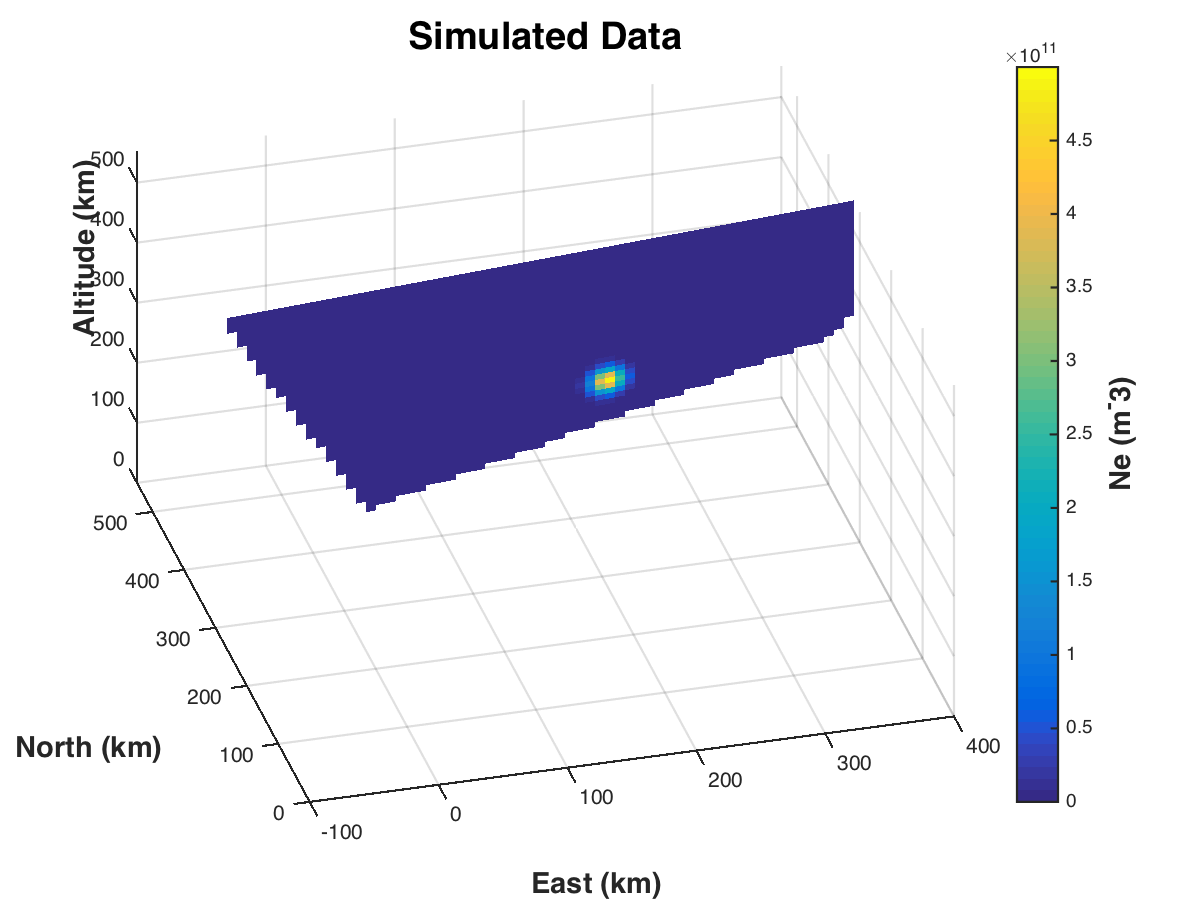
\includegraphics[width=3.5in]{simdataplaneorig}
	\caption{A possible distribution of electron density with a Gaussian shaped enhancement that has a max of 5x10$^{11}$ m$^{-3}$  a standard deviations of 12.7 km along the vertical direction and 8.5 km along the horizontal direction. The center of this plotted at the point $\mathbf{r}=[ 225\text{km}, 225 \text{km},335\text{km}]^T$. It is assumed that the density is constant along the direction orthogonal to the plane of motion.}
	\label{fig:simdataplaneorig}
\end{figure}

Applying the space time ambiguity in Figure \ref{fig:rambplane} along with an assumed motion of 500 m/s, which again suggested by the data in Figure \ref{fig:realdataplane3points}, the distribution in Figure \ref{fig:simdataplane} is created. This seems to suggest that the features seen in Figure \ref{fig:realdataplane} could be from physical phenomena that is much smaller than what is shown in the interpolated image. 

\begin{figure}[h!]
	\centering
	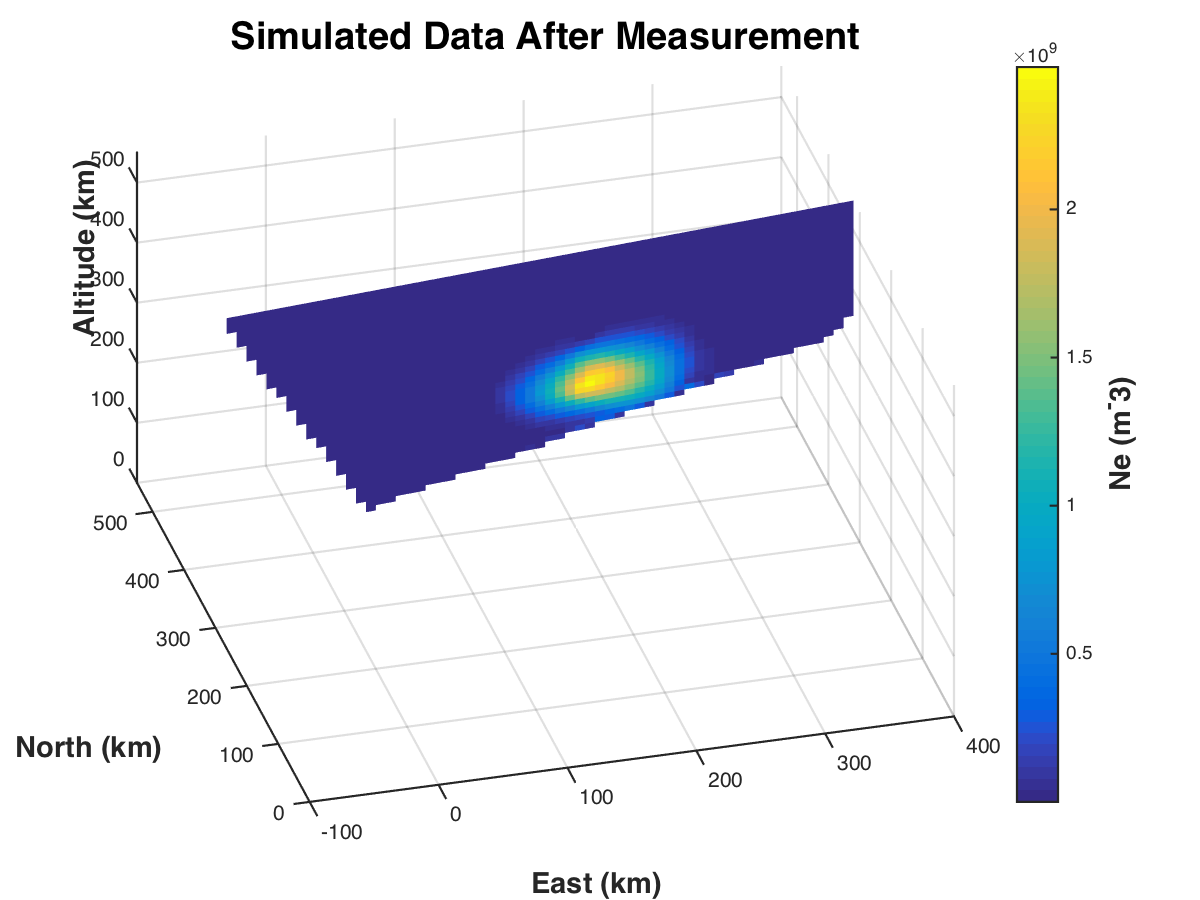
\includegraphics[width=3.5in]{simdataplane}
	\caption{The same feature from Figure \ref{fig:simdataplaneorig} after applying the effect the spatial ambiguity seen in \ref{fig:rambplane} and 500 m/s motion over the two minute integration period.}
	\label{fig:simdataplane}
\end{figure}

\section{Summary}

The use of the Space-Time Ambiguity function as a kernel of Fridholm integral equation is the theoretical framework of this thesis. The process for the estimation of the ACFs fits very well within this mathematical structure. This structure though, is not rigid and can be adapted to the situation that a researcher may face when performing ISR experiments by taking advantage of the fact that the ambiguity kernel is a set of separable functions. The ambiguity can be used similar as a blurring kernel if there is plasma motion which can allow one to set of different possible features, thus creating an ill-posed inverse problem. Lastly, the impact of the ambiguity function can be demonstrated in experiments where real data is used.

Ambiguity function can greatly augment the features seen in the ISR data. The changes one sees are also highly dependent on the interpolation scheme beam pattern and motion of the plasma during the integration time. It is utmost importance that researchers take this impact into account when analyzing ISR data and experiments. The following chapters will show a tool to help predict the impact of the ambiguity and a set of algorithms to reduce its impact.
\cleardoublepage

% -------------------------------------
% CHAPTER 4: STISRS
% -------------------------------------
\chapter{ISR Simulation}
\label{chapter:stisrs}
\thispagestyle{myheadings}

% set this to the location of the figures for this chapter. it may
% also want to be ../Figures/2_Body/ or something. make sure that
% it has a trailing directory separator (i.e., '/')!
\graphicspath{{4_STISRS/Figures/}}

%%%%%%%%%%%%%%%%%%%%%%%%%%%%%%%%%%%%%%%%%%%%%%%%%%%%%%%%%%%%%%%%%%%%%%%%%

The following chapter will detail the methodology behind SimISR along with some processed examples. The first section will show how the synthetic data is created at complex voltage level. After which results of these simulations will be shown after the data has been processed as shown in Section \ref{section:isrproc}. The results will then be interpolated back to the original Cartesian space of the plasma parameters. 

\section{Simulation Methodology}
\label{sec:simmeth}
The SimISR software package allows one to analyze different  experiment scenarios by simulating the ISR measurement process. %The space-time ambiguity is modeled using a coordinate transform and the pulse as a window along range while the statistical error is taken into account by creating complex shaped Gaussian noise.  
% JOHN:   The above  sentence seems unclear.  Is the adjusted version below accurate?  
% Josh: That is correct, although I have to make sure I mention the use of the pulse as a window function that creates the range ambiguity. I believe I do this later on but I have to check.
The space-time ambiguity is modeled through a three-dimensional blurring kernel along with appropriate coordinate transformations to account for target variation during radar acquisition.   The statistical error is taken into account by creating complex shaped Gaussian noise.    
In what follows we begin with a description of construction of spectral filters designed to create the noise-like signal received in ISR experiments. This is followed by description of the process of creating complex receiver voltage data. The last portion will detail the processing used to create statistical estimates of ACFs.

\subsection{Creating Filters}

The simulator takes as input a discretized set of ionosphere state parameters in Cartesian coordinates which can vary in time.  This corresponds to the true field we seek to reconstruct. The first step in the simulator is to create theoretical ISR spectra at each point from the prescribed parameters. For details on calculating these spectra from the intrinsic plasma parameters see, e.g., \cite{kudeki:milla:1} and \cite{kudeki:milla:2}. 

Once the spectra have been created, the simulator transforms the resulting values to a radar-centered spherical coordinate system. This coordinate change acts as a linear operator in spatial dimensions, and the spectra are accordingly weighted and averaged. The weighting in azimuth and elevation is determined by the antenna beam pattern, while the weighting in range (i.e. along beam) is simply a binary test of whether the spectra are within the range gate. If there are no spectra within the range gate, a nearest neighbor rule is used which selects the closest point in Cartesian space. This method to create the spectra for each point is an acceptable approximation because spatial correlations between the electron density fluctuations will be on the order of the Debye length \cite{farley1969} which is, in nearly all practical cases, significantly smaller than the beam width or range gate size. This is same as making the assumption of wide-sense stationarity with uncorrelated scattering (WSSUS)\cite{Kailath:1962jx}. The algorithm implementing spatial sampling is shown in the simplified diagram in Figure \ref{fig:beamdia}.

\begin{figure}[!t]
\centering
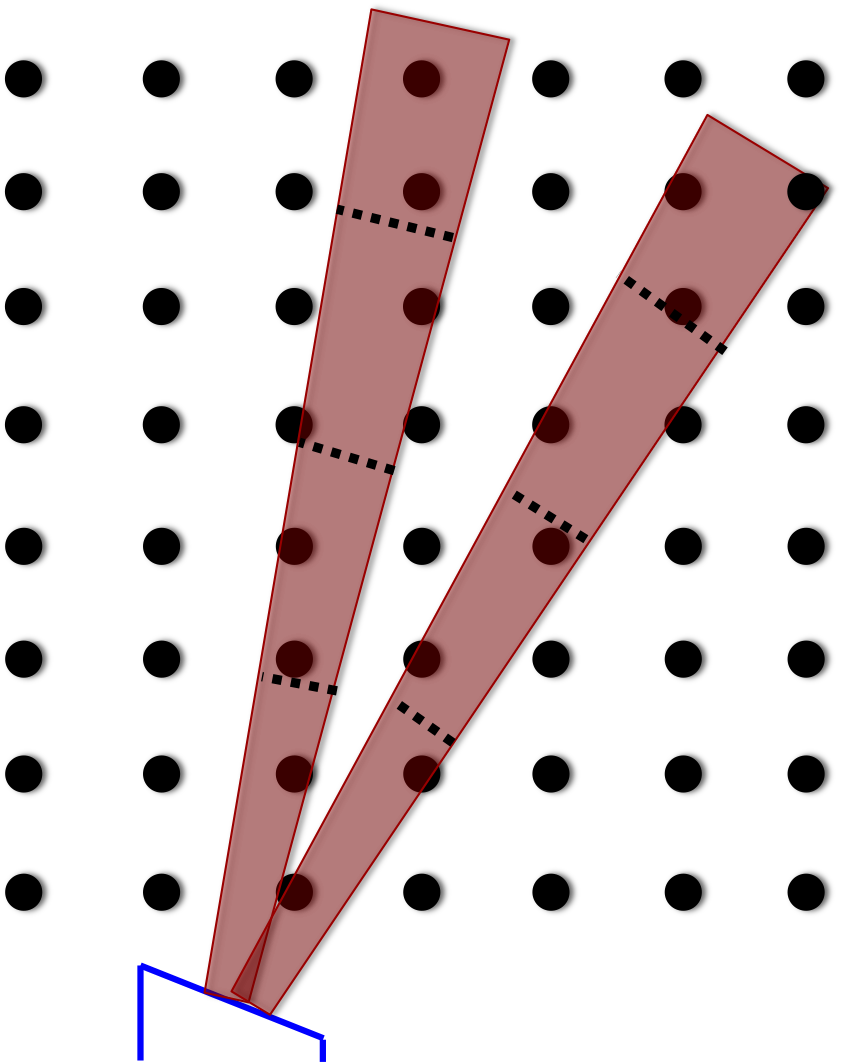
\includegraphics[width=2in]{beamsampling}
\caption{Each point is a from a discrete sampling of a Cartesian space. The beams are broken up into range gates, separated by the dotted lines, and the parameters at each point overlapping within these gates are averaged.}
\label{fig:beamdia}
\end{figure}
 
% Once the spectrum at the specific point in range and angle space has been determined, the filter $H_m(\omega)$, is created by simply taking the square root of the spectrum, $S_m(\omega | \: \bm{\theta})$,

% \begin{equation}
% \label{eq1}
% H_m(\omega) = \sqrt{S_m(\omega | \: \bm{\theta})}.
% \end{equation}

Once the theoretical spectrum for a given scattering volume has been calculated, an appropriate spectral shaping filter is created. The method to create the filter given a desired spectrum or ACF can be done in a number of ways \cite{Kasdin:1995wi}. The implementation in SimISR creates an infinite impulse response filter in order to ensure a causal, minimum phase filter. 
%% PJE: Why does SimISR pick an IIR filter, which is not guaranteed to have a linear phase response across the passband (i.e. constant delay)?  Might be worth a comment here.
%% JPS: This creates a causal, minimum phase filter. It may not be linear phase but its not necessarily need in this application as we are not worried about dispersion of the input signal. The filters just need to be stable and the causality allows one to use the minimum phase assumption to justify stability.
The coefficients are determined using the ACF by solving the following set of equations,

\begin{equation}
\label{eq:filtereq}
\begin{bmatrix} R_m(0) & R_m(1)& \cdots & R_m(L-1) \\ R_m(L-1) & R_m(0)& \cdots & R_m(L-2)\\ \vdots & &\ddots  & \vdots \\  R_m(1) & R_m(2) & \cdots & R_m(0) \end{bmatrix} \left[ \begin{array}{c} a_1\\ a_2\\\vdots \\ a_L \end{array} \right]=\left[ \begin{array}{c} R_m(1) \\ R_m(2)\\ \vdots \\R_m(L) \end{array} \right]
\end{equation}

\noindent where $R_m(l)$ are the ACF values, $L$ is the desired length of the filter, and $ a_i$ are the set of filter coefficients. The filter then takes the form in the frequency domain as the following,

\begin{equation}
\label{eq:filtz}
H_m(z) = \frac{G}{1-\displaystyle \sum_{l=1}^{L} a_l z^{-l}}.
\end{equation}
\noindent The gain term $G$ is used to make sure the noise has the correct variance. This can be calculated as 

\begin{equation}
\label{eq:gainterm}
G=\sqrt{\displaystyle \sum_{l=0}^L -a_l R_m(l)},
\end{equation}

\noindent where $a_0=-1$. This method has been used in similar ways in other contexts--e.g., the creation of vocoders for speech processing applications, as it creates causal and stable filters \cite{rabinerdigitalspeech}.
%\noindent The term $ \bm{\theta}$ refers to the plasma parameters needed to make the spectrum. This filter then is used to create the synthetic IQ data.

\subsection{Simulated Complex Voltage Creation}

The algorithm used to create sampled complex receiver voltages employs a complex white Gaussian noise (CWGN) process (``plant") that is spectrally shaped at its output using a time domain filter. As stated in the previous subsection, each point in space and time will have a separate noise plant and filter which is derived from the plasma and radar parameters parameters. Figure \ref{fig:IQdiagram} presents a representative example. 

\begin{figure}[h!]
\centering

\includegraphics[width=4in]{diagrampart}
\caption{Diagram for complex receiver voltage simulator signal flow.}
\label{fig:IQdiagram}
\end{figure}

The creation of one set of complex receiver voltage data can be represented by

\begin{equation}
\label{eq2}
y_m (k)= s(k)\left[h_m(k)*w(k)\right],
\end{equation}
 
\noindent where $s(k)$ is the overall transmitted pulse envelope, $h_m(k)$ is the time domain representation of the filter in Equation \ref{eq:filtz} and $w(k)\sim CN(0,\mathbf{I})$ or CWGN noise process. The pulse shape acts as a window function, since the plasma will only reflect energy during the time it is illuminated by the radar signal. 
%The application of this filter is actually done in the frequency domain. This is possible because the Discrete Fourier Transform (DFT) of a vector of CWGN is also CWGN. The only difference is that there is a change in the variance, which is tied to the number of points used in the DFT \cite{kayvol1}. With this in mind Equation \ref{eq2} can be implemented as the following,

%\begin{equation}
%\label{eq:fftfilt}
%y_m (k)= s(k)\displaystyle \sum_{i=0}^{K-1}e^{j\omega_ik}\left[ \sqrt{S_m(\omega_i | \: \bm{\theta})}w(\omega_i)\right],
%\end{equation}
%
%\noindent where $\omega_i$ is the frequency variable, $w(\omega_i) \sim CN(0,\mathbf{I})$ and $K$ is the number of points used for the DFT \cite{michellnoisesim1981}.

After the data for each range gate $y_m(k)$ is created, the received signal's power spectrum can be calculated from ISR plasma scattering theory as 

\begin{equation}
\label{eq3}
P_r = \frac{\left(c\Delta T\right) G \lambda^2}{2(4\pi)^2}\frac{P_t }{R^2}\frac{\sigma_e N_e}{(1+k^2\lambda_D^2),(1+k^2\lambda_D^2 + T_r)},
\end{equation}
 
 \noindent where $P_r$ is the power received in Watts (W), $k$ is the wavenumber of the radar in meters (m), $c$ is the speed of light in m/s, $\Delta T$ is the along-range gate extent in seconds, $G$ is the gain of the antenna, $P_t$ is the power of the transmitter in W, $\sigma_e$ is the electron radar cross section in $m^2$,  $\lambda_D$ is the Debye length in m, $N_e$ is the electron density in m$^{-3}$, and $T_r$ is the electron to ion temperature ratio.
  
The received signal power calculated at each range gate using Equation~\ref{eq3} is used as a scaling constant for each $y_m(k)$ series.  A delayed and summed operator yields a model of the received radar scatter signal:
 
\begin{equation}
\label{eq4}
x(n) = \displaystyle\sum\limits_{m =0}^{M-1} \alpha(m)y_m(n-m),
\end{equation}

\noindent where $\alpha(m) = \sqrt{P_r(m)}/\widehat{\sigma}_y$ and $\widehat{\sigma}_y$ is the estimate of the standard deviation of $y_m(k)$. Lastly, to model total noise from the radar system and environment, an additive CWGN process is included, creating the final simulated complex receiver voltage sequence

\begin{equation}
\label{eq:addnoise}
x_f(n) = x(n) +\sqrt{\frac{k_bT_{sys}B}{2}} w(n), \quad w(k)\sim CN(0,\mathbf{I})
\end{equation}

\noindent where $k_b$ is Boltzmann's constant, $T_{sys}$ is the system temperature and $B$ is the system bandwidth.
A full diagram of the model can be seen in Figure \ref{fig:isrdiag}.

\begin{figure}[!h]
\centering

\includegraphics[width=5.5in]{diagram}
\caption{ISR simulation diagram.}
\label{fig:isrdiag}
\end{figure}
\section{Simulation Examples}
\label{sec:simex}

The framework for SimISR allows exploration of a number of aspects of ISR processing. Within the scope of this article, we will focus on four application examples.

The first example compares the output of SimISR with a set of relatively quiet data from the PFISR system. The next case demonstrates how the simulator can be used for Monte Carlo estimates of ISR spectra. In this case, we hold all of the plasma parameters constant and determine how the distribution of the measured parameters evolve. The next example uses a simple altitude distribution of ionospheric plasma parameters to show the impact of the forward model of the ISR on a basic measurement of electron density. This is intended to illustrate that basic ambiguities inherent in ISR measurements can give the appearance of a change in morphology of the plasma phenomena when none truly exists. Finally, the output of a fully consistent multi-fluid ionosphere model is used as input to the ISR simulator and is applied in two use cases relevant to experiment planning, one varying over two spatial dimensions and another varying in all three spatial dimensions. The results of these use cases illustrate an inherent tradeoff in experiment construction between reducing statistical fluctuations in the measurement and increasing distortion in the final reconstruction. 

\subsection{Real Data Comparison}

The first example shows PFISR data compared to SimISR. This comparison is made up of an altitude profile taken from PFISR during a quiescent period during the day. An input set of parameters was created using analytic funtions that resemble the data from the radar. A Chapman function for the electron density; arctan functions for the ion and electron temperatures; and constant of zero for the ion velocities.

The chosen parameters for the inputs can be seen in Figure \ref{fig:simisrparamcomp} as the green lines. The collected PFISR data can be seen in blue and the SimISR output in red. The plots show that the PFISR and SimISR data show similar variability within the parameters.


\begin{figure}[h!]
\centering
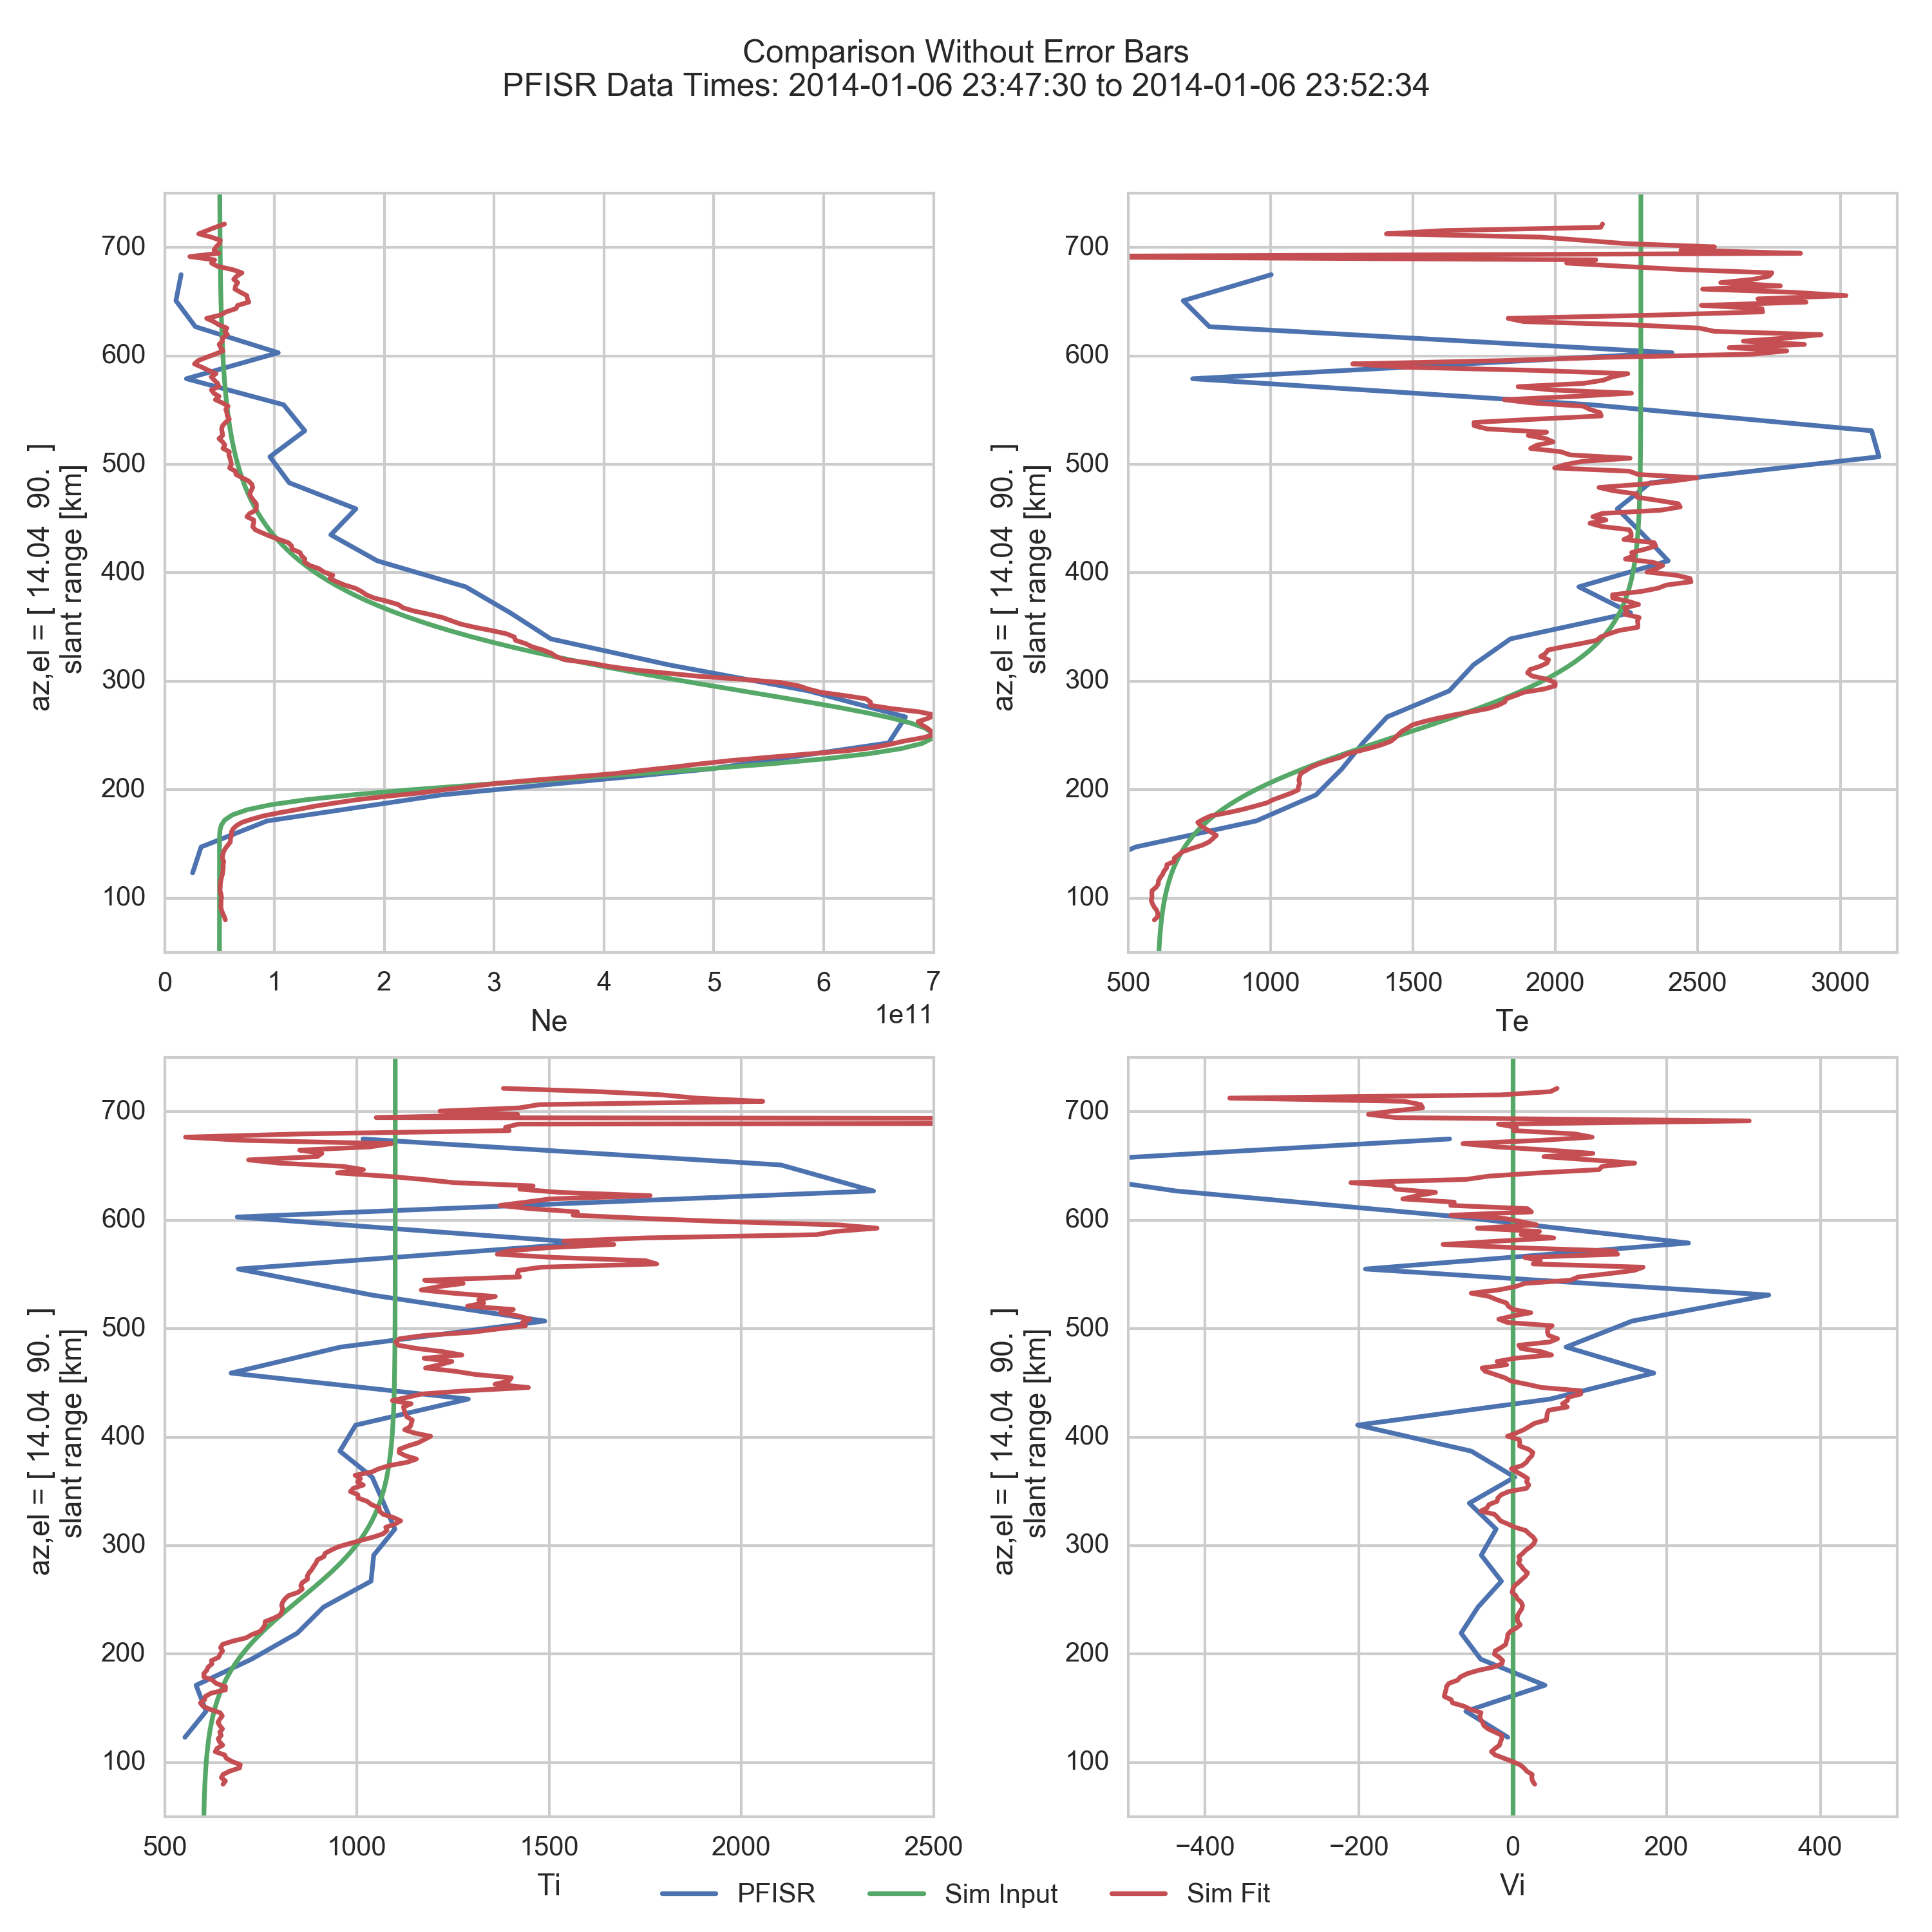
\includegraphics[width=4.5in]{Paramcomp}
\caption{Comparison of real data from PFISR with SimISR data and a possible input parameter distribution.}
\label{fig:simisrparamcomp}
\end{figure}

A version of Figure \ref{fig:simisrparamcomp} can be seen with error bars in Figure \ref{fig:simisrparamcompeb}. The error bars in the SimISR parameters seem to be much small than those from PFISR. This could be due to a number of reasons including slightly different fitting algorithms.

\begin{figure}[h!]
\centering
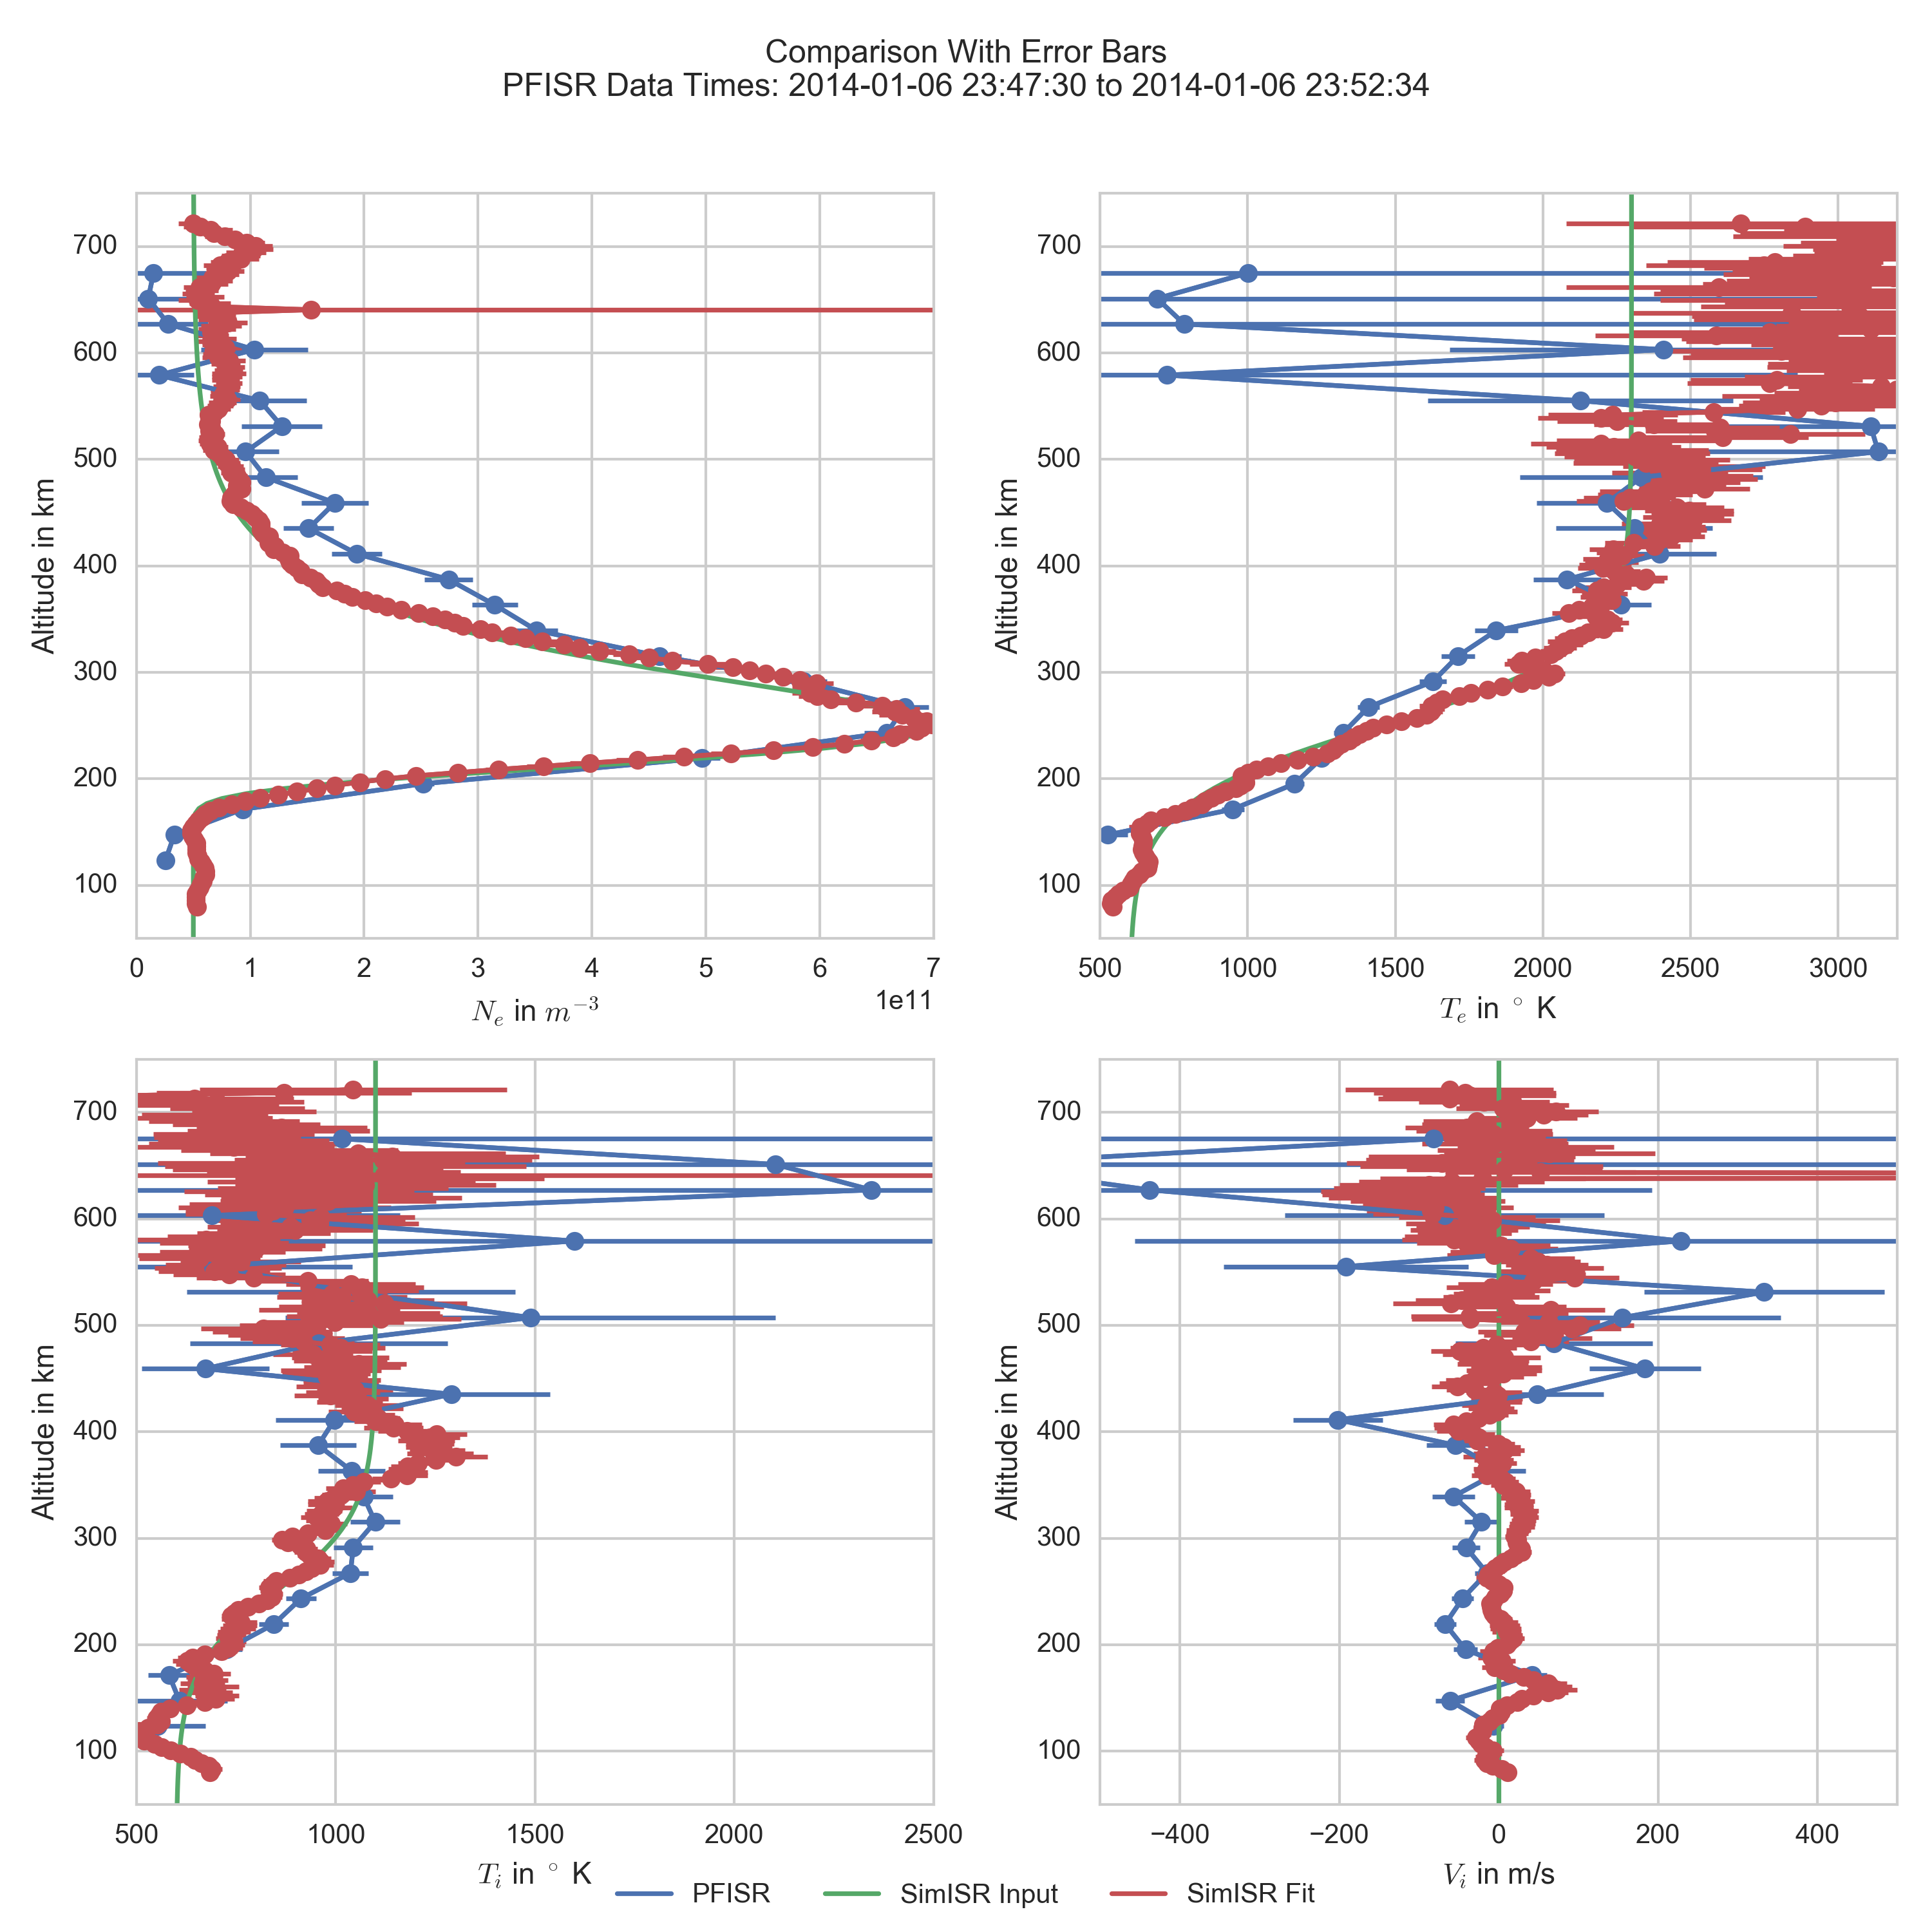
\includegraphics[width=4.5in]{Paramcompeb}
\caption{Comparison of real data from PFISR with SimISR data and a possible input parameter distribution along with error bars.}
\label{fig:simisrparamcompeb}
\end{figure}

Lastly a comparison of example ACFs and spectra are shown in Figure \ref{fig:simisrspectcom}. This shows relatively good correspondence between PFISR and SimISR. 

\begin{figure}[h!]
\centering
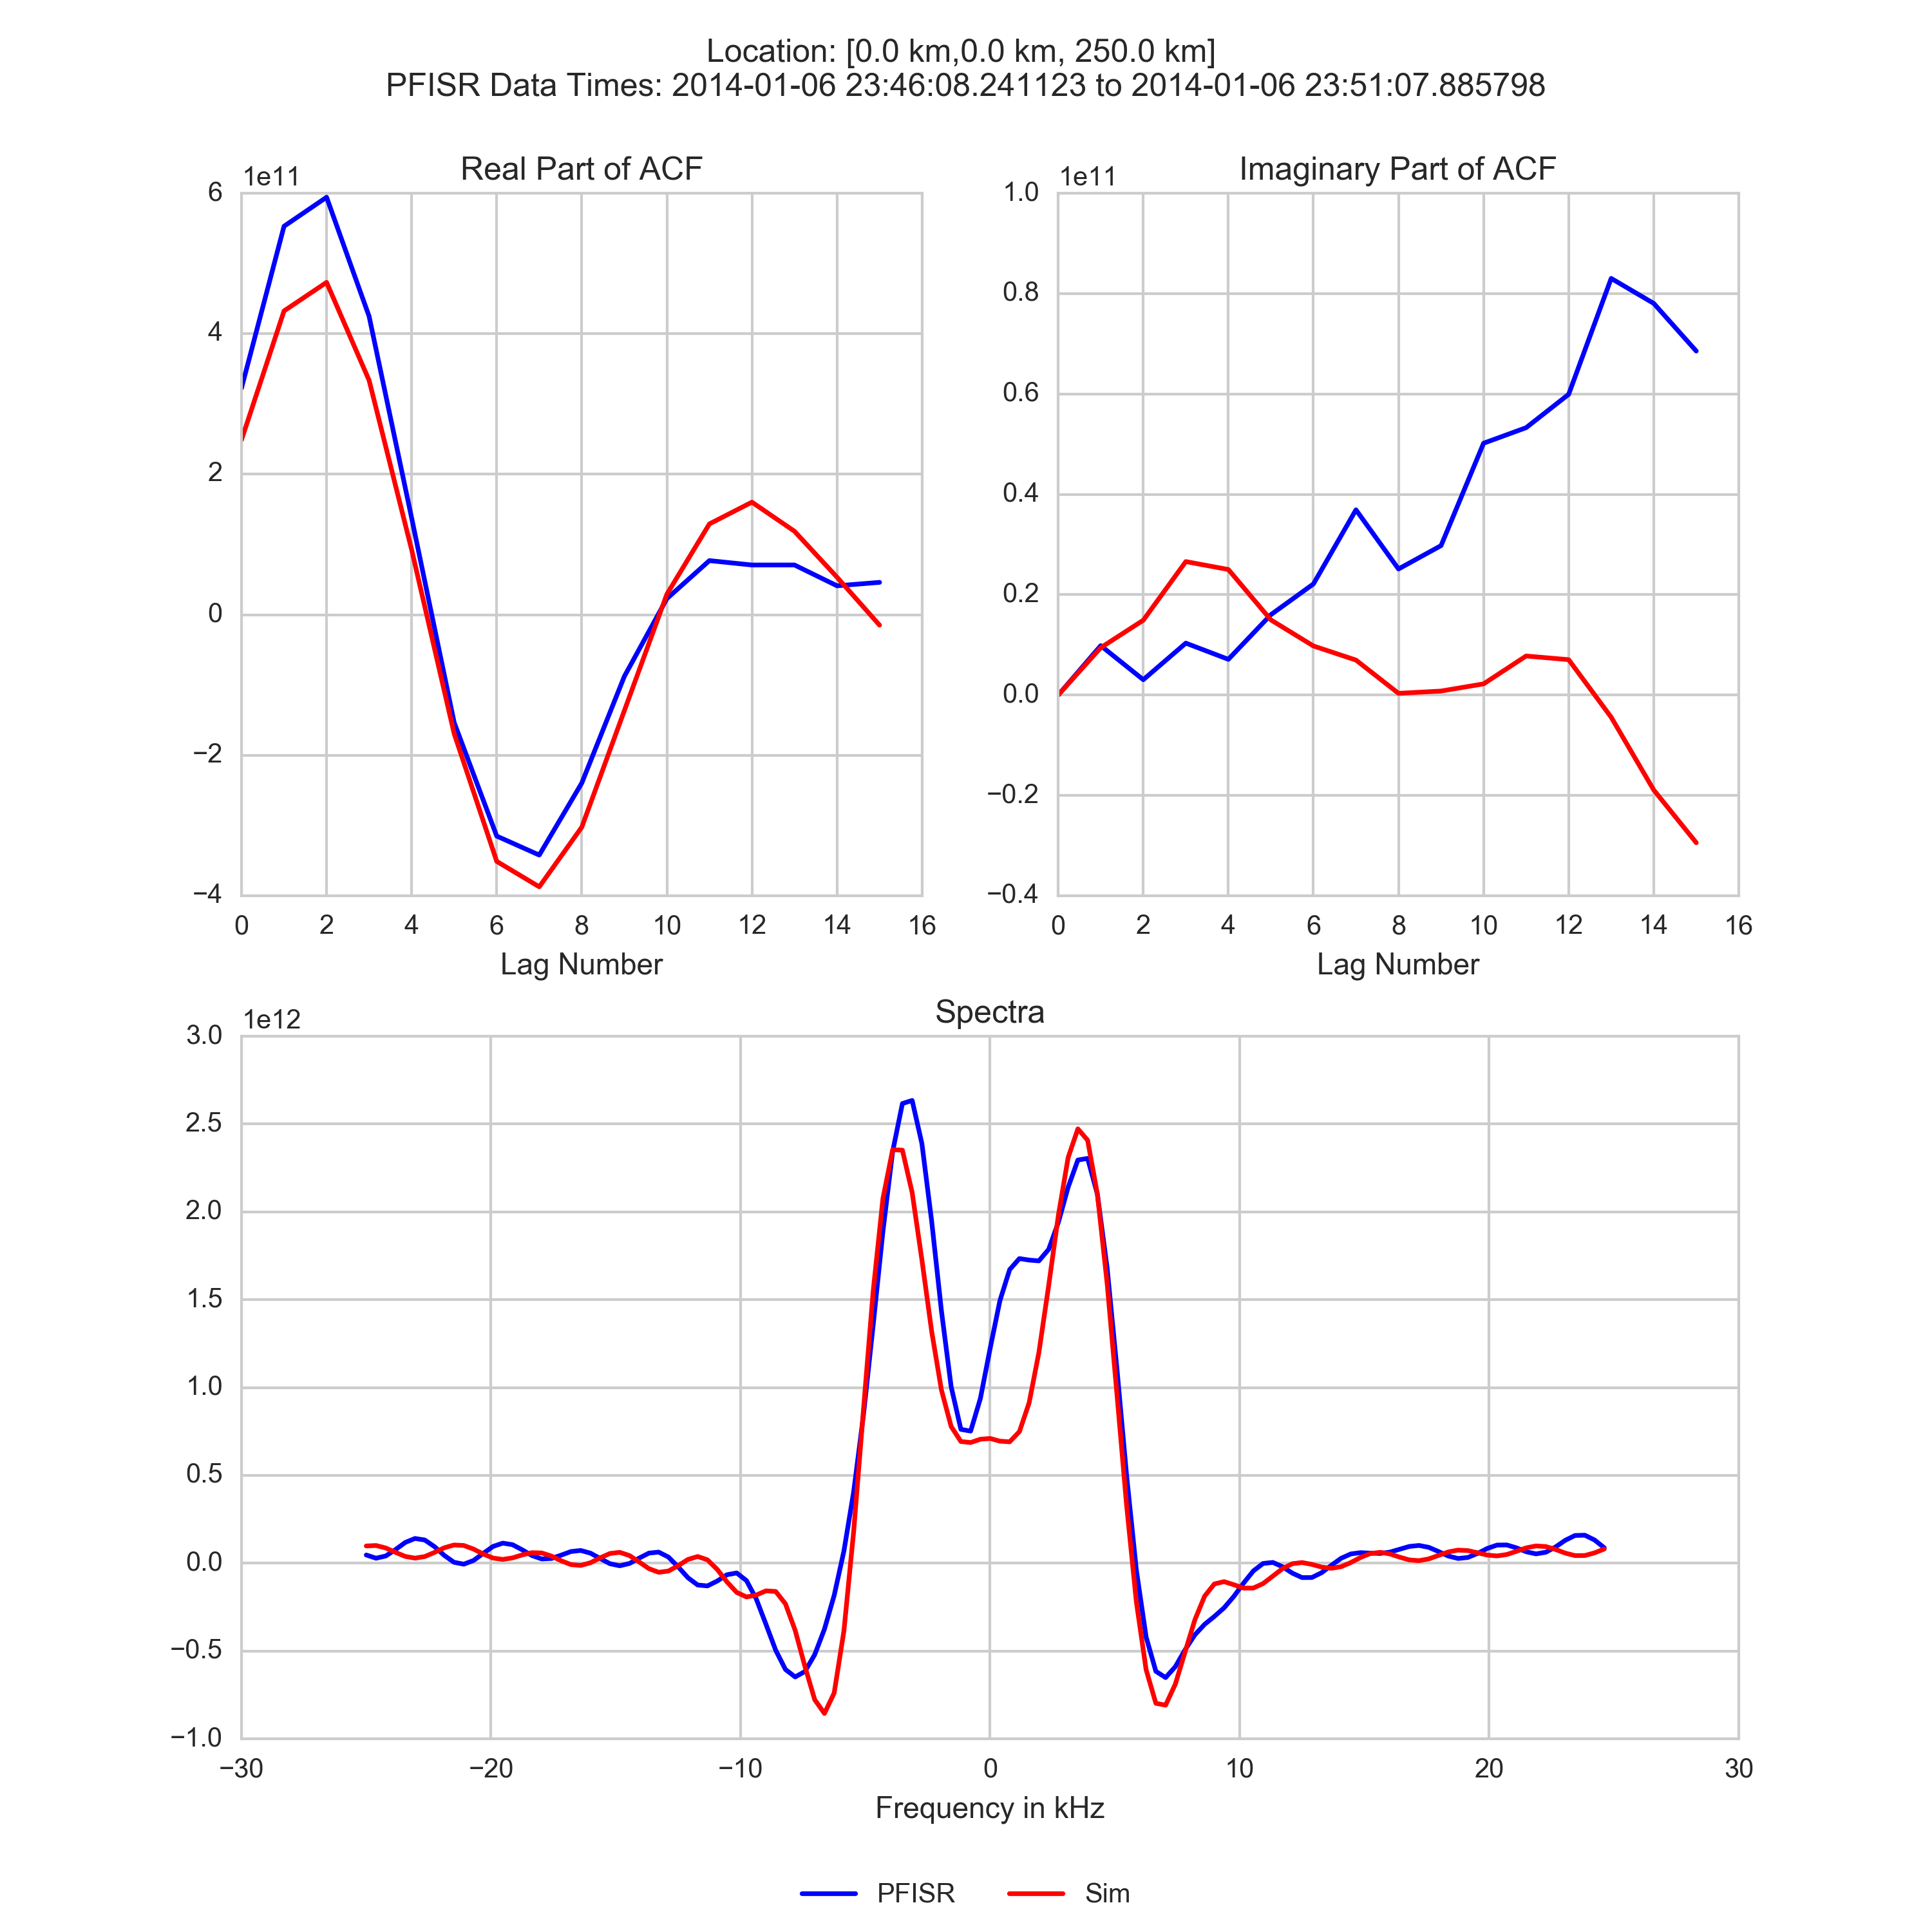
\includegraphics[width=4.5in]{speccomp}
\caption{Comparison of ACFs and spectra from PFISR with SimISR.}
\label{fig:simisrspectcom}
\end{figure}

\subsection{Monte Carlo Example}

It is often necessary to obtain a large number of sensor measurements for a statistical study or for creating of a training data set for a pattern recognition algorithm. This can be a very burdensome search and classification task for the researcher if the input set must be drawn from actual sensor measurements. However, a number of useful cases exist where SimISR can be profitably employed to create a synthetic data set instead, saving considerable work over case assembly from a real ISR data based training set.  We explore one such example in this section.

% JOHN: you still need to work on this comment by Phil, no?   :
%\pcom{Very awkward and verbose; rewrite}{It is necessary to understand the statistics from the sensors used in scientific studies. In order to do this a large number of measurements must be taken with the sensor. There are issues with this approach in that the inputs can not be controlled so along with any random variation that may be found in the sensor the random variation of the measured process will be included and must be taken into account during the analysis of the data. With the simulator the statistical fluctuations from only the measurement mechanism only can be studied and thus reducing the uncertainty of the measurements.}
% Josh I updated the above paragraph to take care of Phil's comment. The point of the paragraph is I can make a training set instead of working through a data base to collect and classify data. Perhaps I can add a reference to pattern recognition book that talks about training sets.
For this example we show how distributions of plasma parameter measurements change as more pulses are averaged. To do this we created a field of constant plasma parameters typical of the high latitude ionosphere at around 250 km, and performed a Monte Carlo-type simulated statistical experiment using a number of independent realizations. We use the parameters for the Poker Flat AMISR system for this simulation along with the plasma parameter listed in Table \ref{tb:param1}. For a number of independent radar pulse counts, $J$, we used 4,600 realizations of the statistical ISR measurement process in each case to create statistical distributions of measured parameter values. To calculate distributions histograms are created using each of these relations, although some come from the same beam and thus there can be some statistical correlation. The distributions can be seen in Figure \ref{fig:statshistall} which show distributions where 200, 500 and 1000 pulses are used respectively. For a given pulse count $J$, the plasma parameters have a Gaussian-like distribution. As expected the distribution narrows as the number of pulses $J$ is increased. Another observation is that as the number of pulses increases the bias in the measurement is reduced, which could be due to the way that the histograms were calculated.
%% PJE:  However, Figure 5 clearly shows a biased measurement for the 200 pulse case slowly resolving to zero bias in the 500 and 1000 sample cases.  You need to address this behavior here, as a sharp reviewer is going to notice and call it out.  I don't offhand know why that is happening.
%% JPS: Didn't have a great answer, I have a feeling that it might be related to how I calculated the histograms. I took data from all of the beams together so there correlations between some samples. The  
%% PJE: I guess then you need to leave it alone, but I would be prepared for questions.
%% JLS:  So it doesn’t actually resolve to 0, at least in the density histogram.  For large number of pulses there seems to be a second bump at 0.7e11.   Would it be worth looking at some ACF fits for those cases to try and see if there is some obvious explanation?  Are you adding receiver/sky noise for these runs?   Could incorrect noise subtraction, or maybe some coloring in the noise generation, be a cause?  I’m confident that a reviewer will raise this issue, so best to just get our response together now!
\begin{table}[!t]
\centering
\caption{Simulation parameters.}
\label{tb:param1}
\begin{tabular}{ll}
Species & O+ e-\\
$N_e$    & $1\times 10^{11}$ \\
$T_e$      & $2100^o$ K   \\
$T_i$      & $1100^o$ K \\
$V_i$      & $0$ m/s
\end{tabular}
\end{table}

\begin{figure}[!t]
\centering
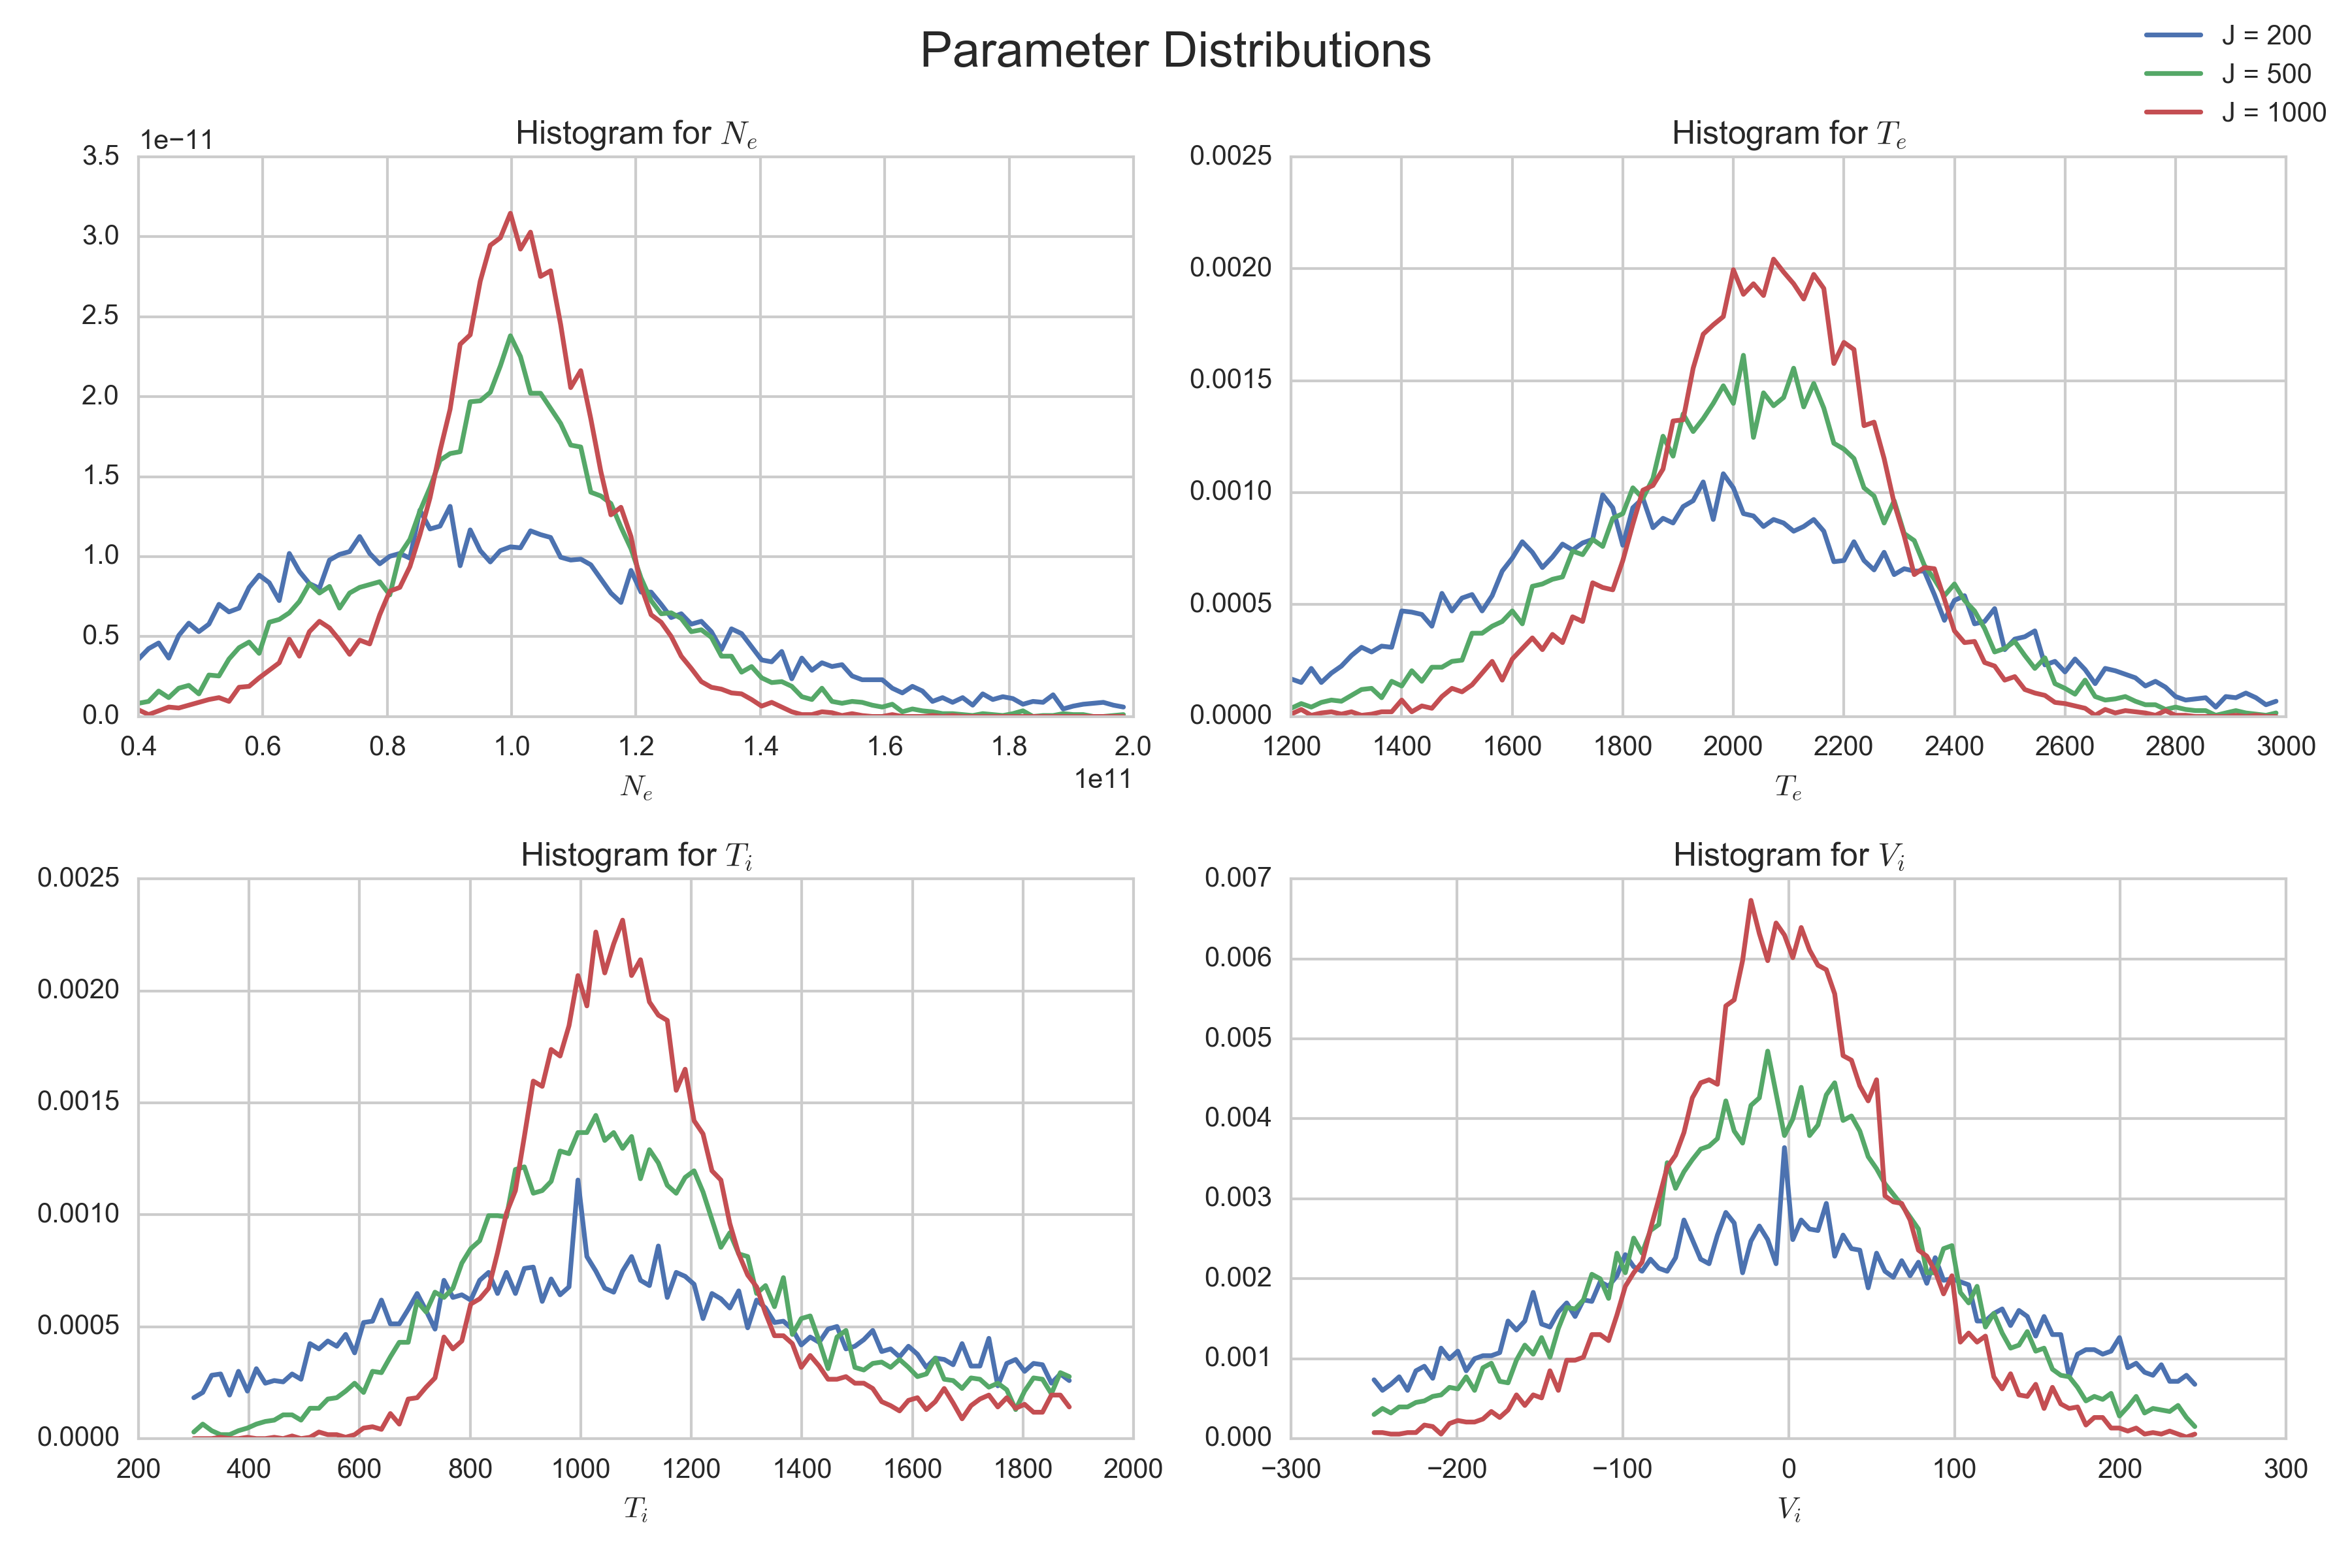
\includegraphics[width=5in]{datahist}
\caption{Normalized histograms of fitted plasma measurements from cases with 200, 500 and 1000 pulses integrated. These are estimates of probability density functions for each of the plasma parameters measurements given the values in Table \ref{tb:param1}.}
\label{fig:statshistall}
\end{figure}

ISR error analysis also benefits from SimISR's ability to generate a large number of samples of fitted parameters. In particiular, ISR measurements need to have estimates of the errors, and accuracy of the estimates of these errors can be explored using SimISR. Using the 1000 pulse case seen in Figure \ref{fig:statshistall}, we can compare simulated output distributions with the actual distribution of parameter values. Figure \ref{fig:statshistsingle} shows a comparison of these two different models using. The first method, represented by the blue line, uses the sample mean and variance calculated from each as the variance and mean for a Normal distribution. The other method, which generated the green line, calculates an average squared error from the true value for each parameter for the variance in a Normal distribution and uses the true value for the mean. 
%% PJE: I'm confused by the logic of this sentence above (also "shows gives" etc?) - please reword.
%% JPS: Just changed 
This example shows that the parameter distributions are well represented by a Gaussian function but that the error estimated from the fit may not give a completely accurate representation of variance of these parameters. 

\begin{figure}[!t]
\centering
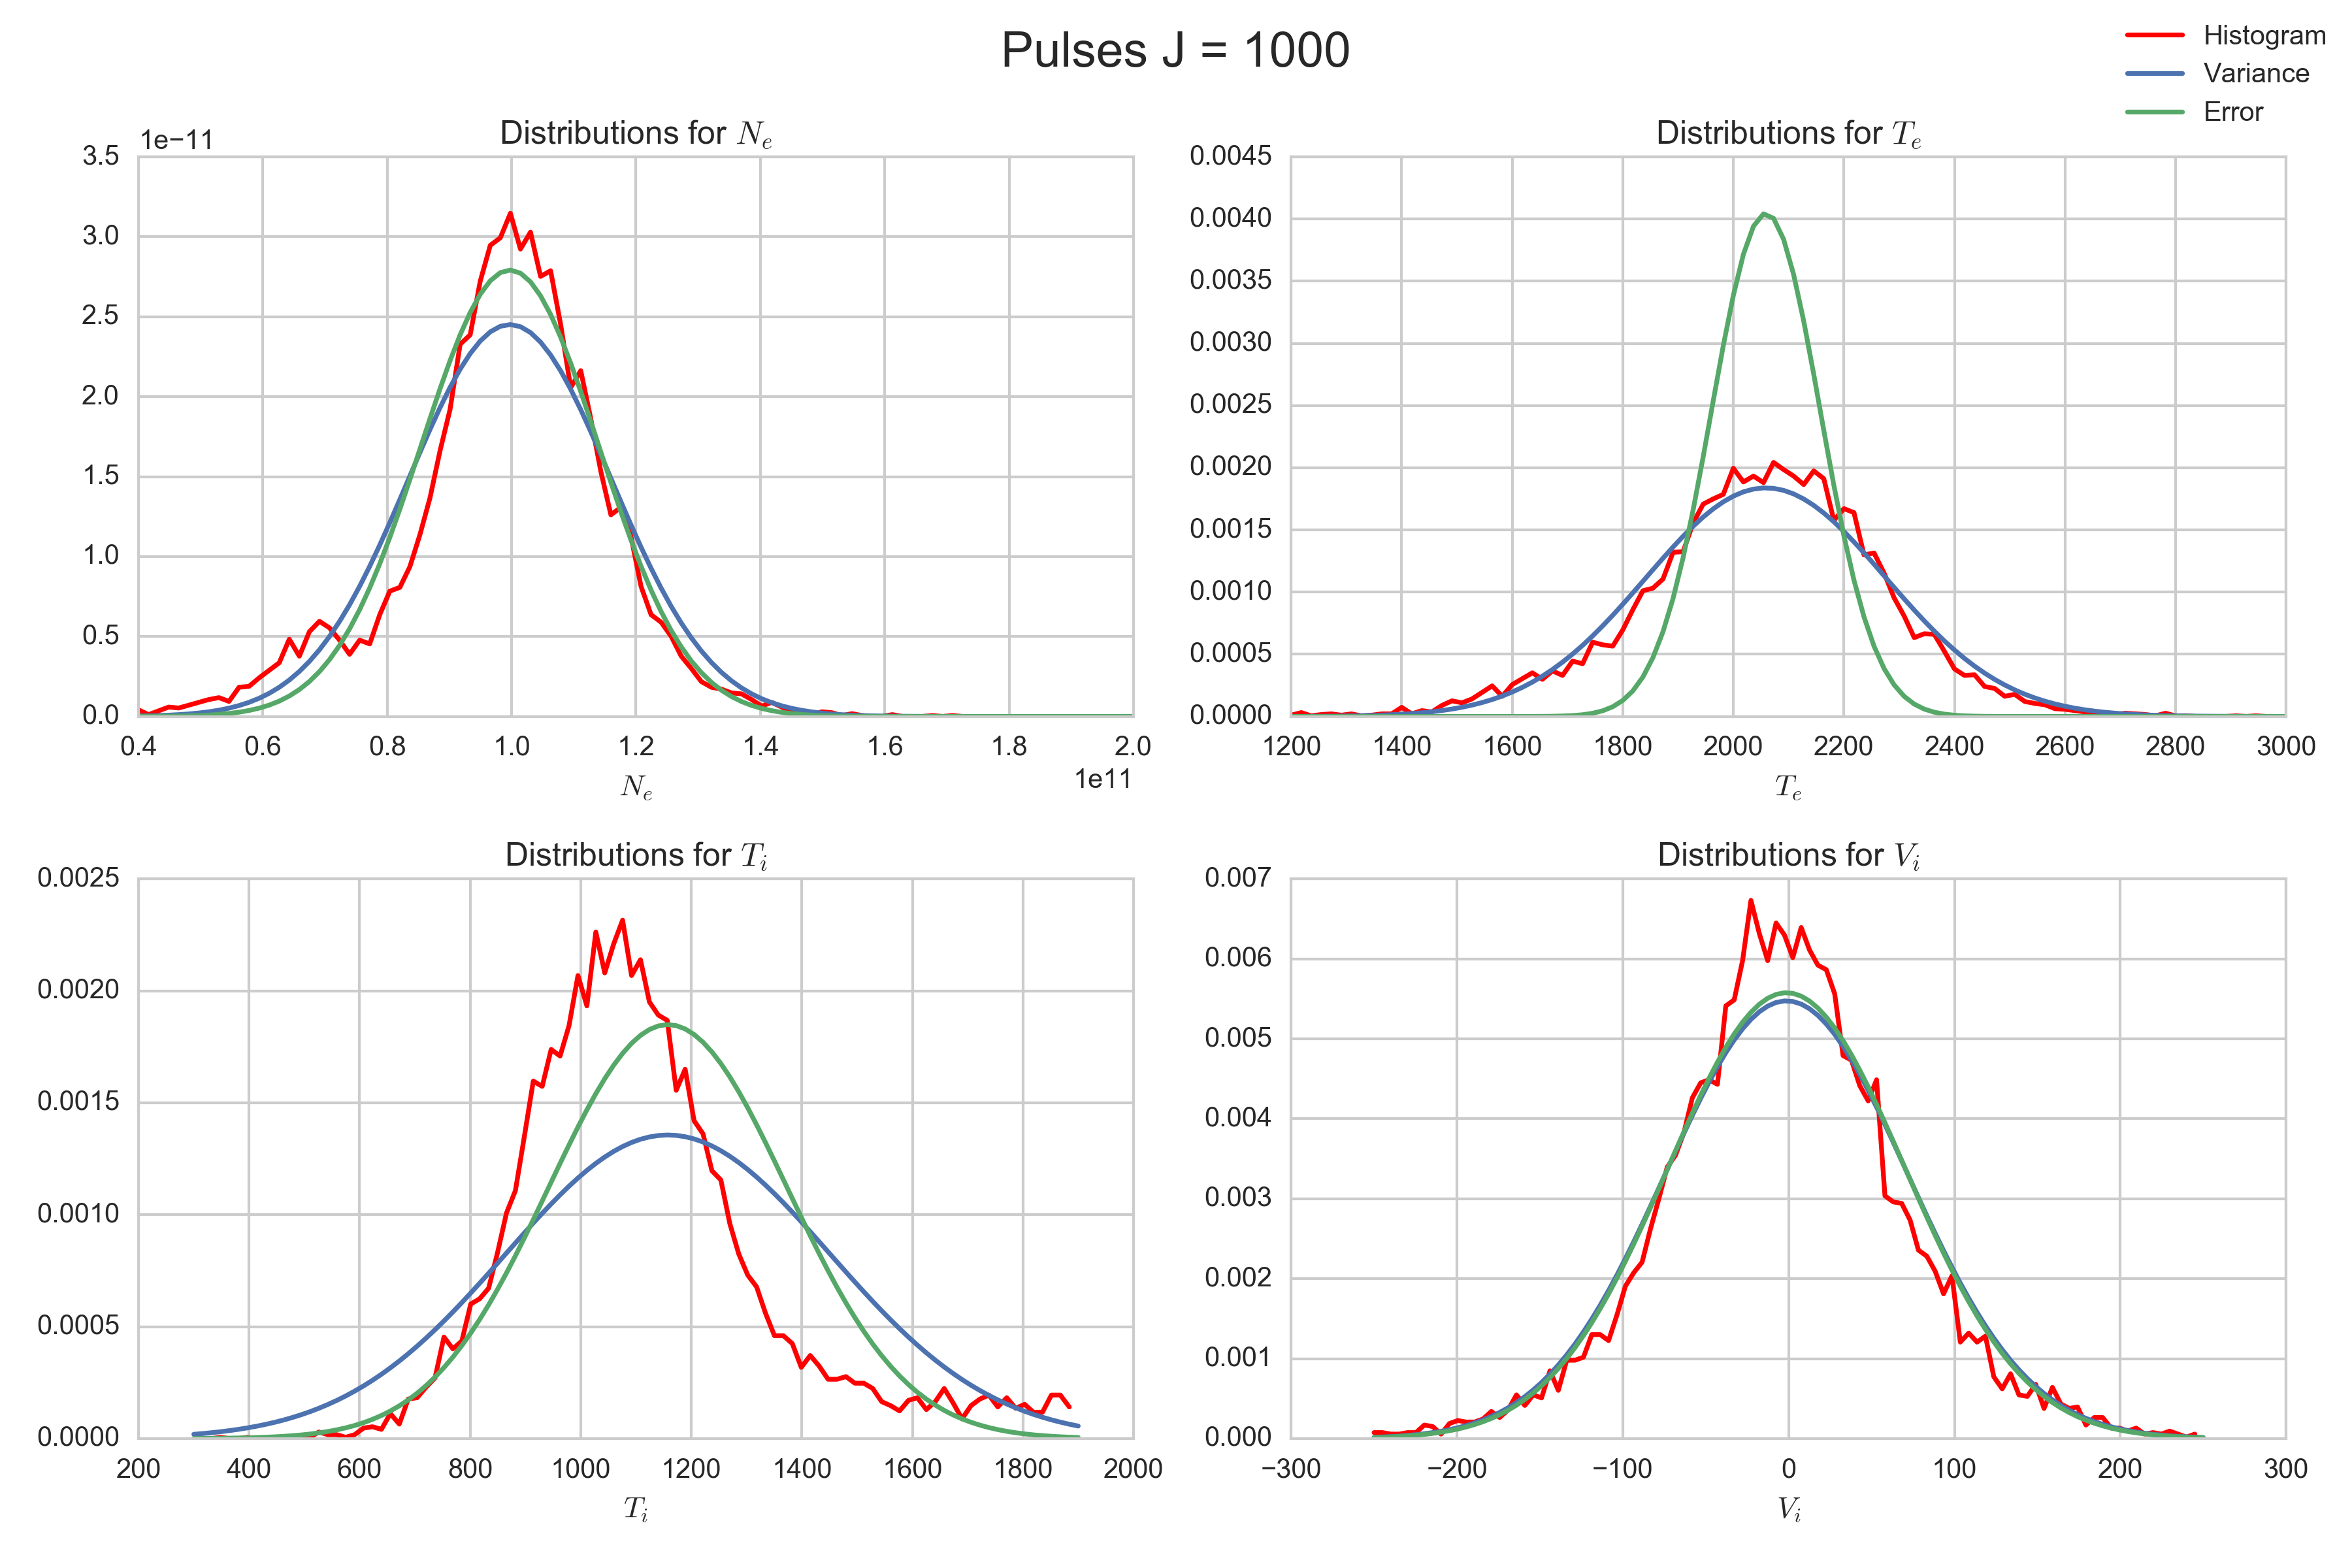
\includegraphics[width=5in]{histsingle}
\caption{Distributions of fitted plasma measurements from cases with 1000 pulses integrated. The red curve shows the actual distribution derived from a histogram of 4600 measurements. The blue curve is a Normal distribution using the MSE from the measurements as the variance and the average parameter value as the mean.  The green curve is a Normal distribution using the average estimate of error squared that comes with the parameter measurement as the variance and the average parameter value as the mean.}
\label{fig:statshistsingle}
\end{figure}


The SimISR tool is useful for identifying situations where assumptions in the parameter fitting break down. For example, a number of studies have explored the case where ISR parameter measurements and spectra show evidence of non-Maxwellian plasma behavior (for AMISR examples see)\cite{Akbari:2012dz,Akbari:2015fv}. Future studies using the simulator could help create a training set that can be used with a pattern recognition algorithm to identify cases where normal fitting procedures may be incorrect due to violation of Maxwellian assumptions.

\subsection{Electron Density Measurement}
An important aspect of experiment design is determining the observability of plasma phenomena with ISR. The simulator can be used to help understand the trade space accompanying a given experimental configuration. With this in mind, we use a simple two dimensional spatial field of ionospheric parameters as an illustrative case study. An all-O$^+$ ionosphere is created with a background electron density that follows a Chapman function with $1\times10^{11}$ m$^{-3}$ as the peak value and a constant electron and ion temperatures of 2000 K and 1500 K respectively. The background ionosphere is depicted in Figure \ref{fig:background1}.

\begin{figure}[!t]
\centering
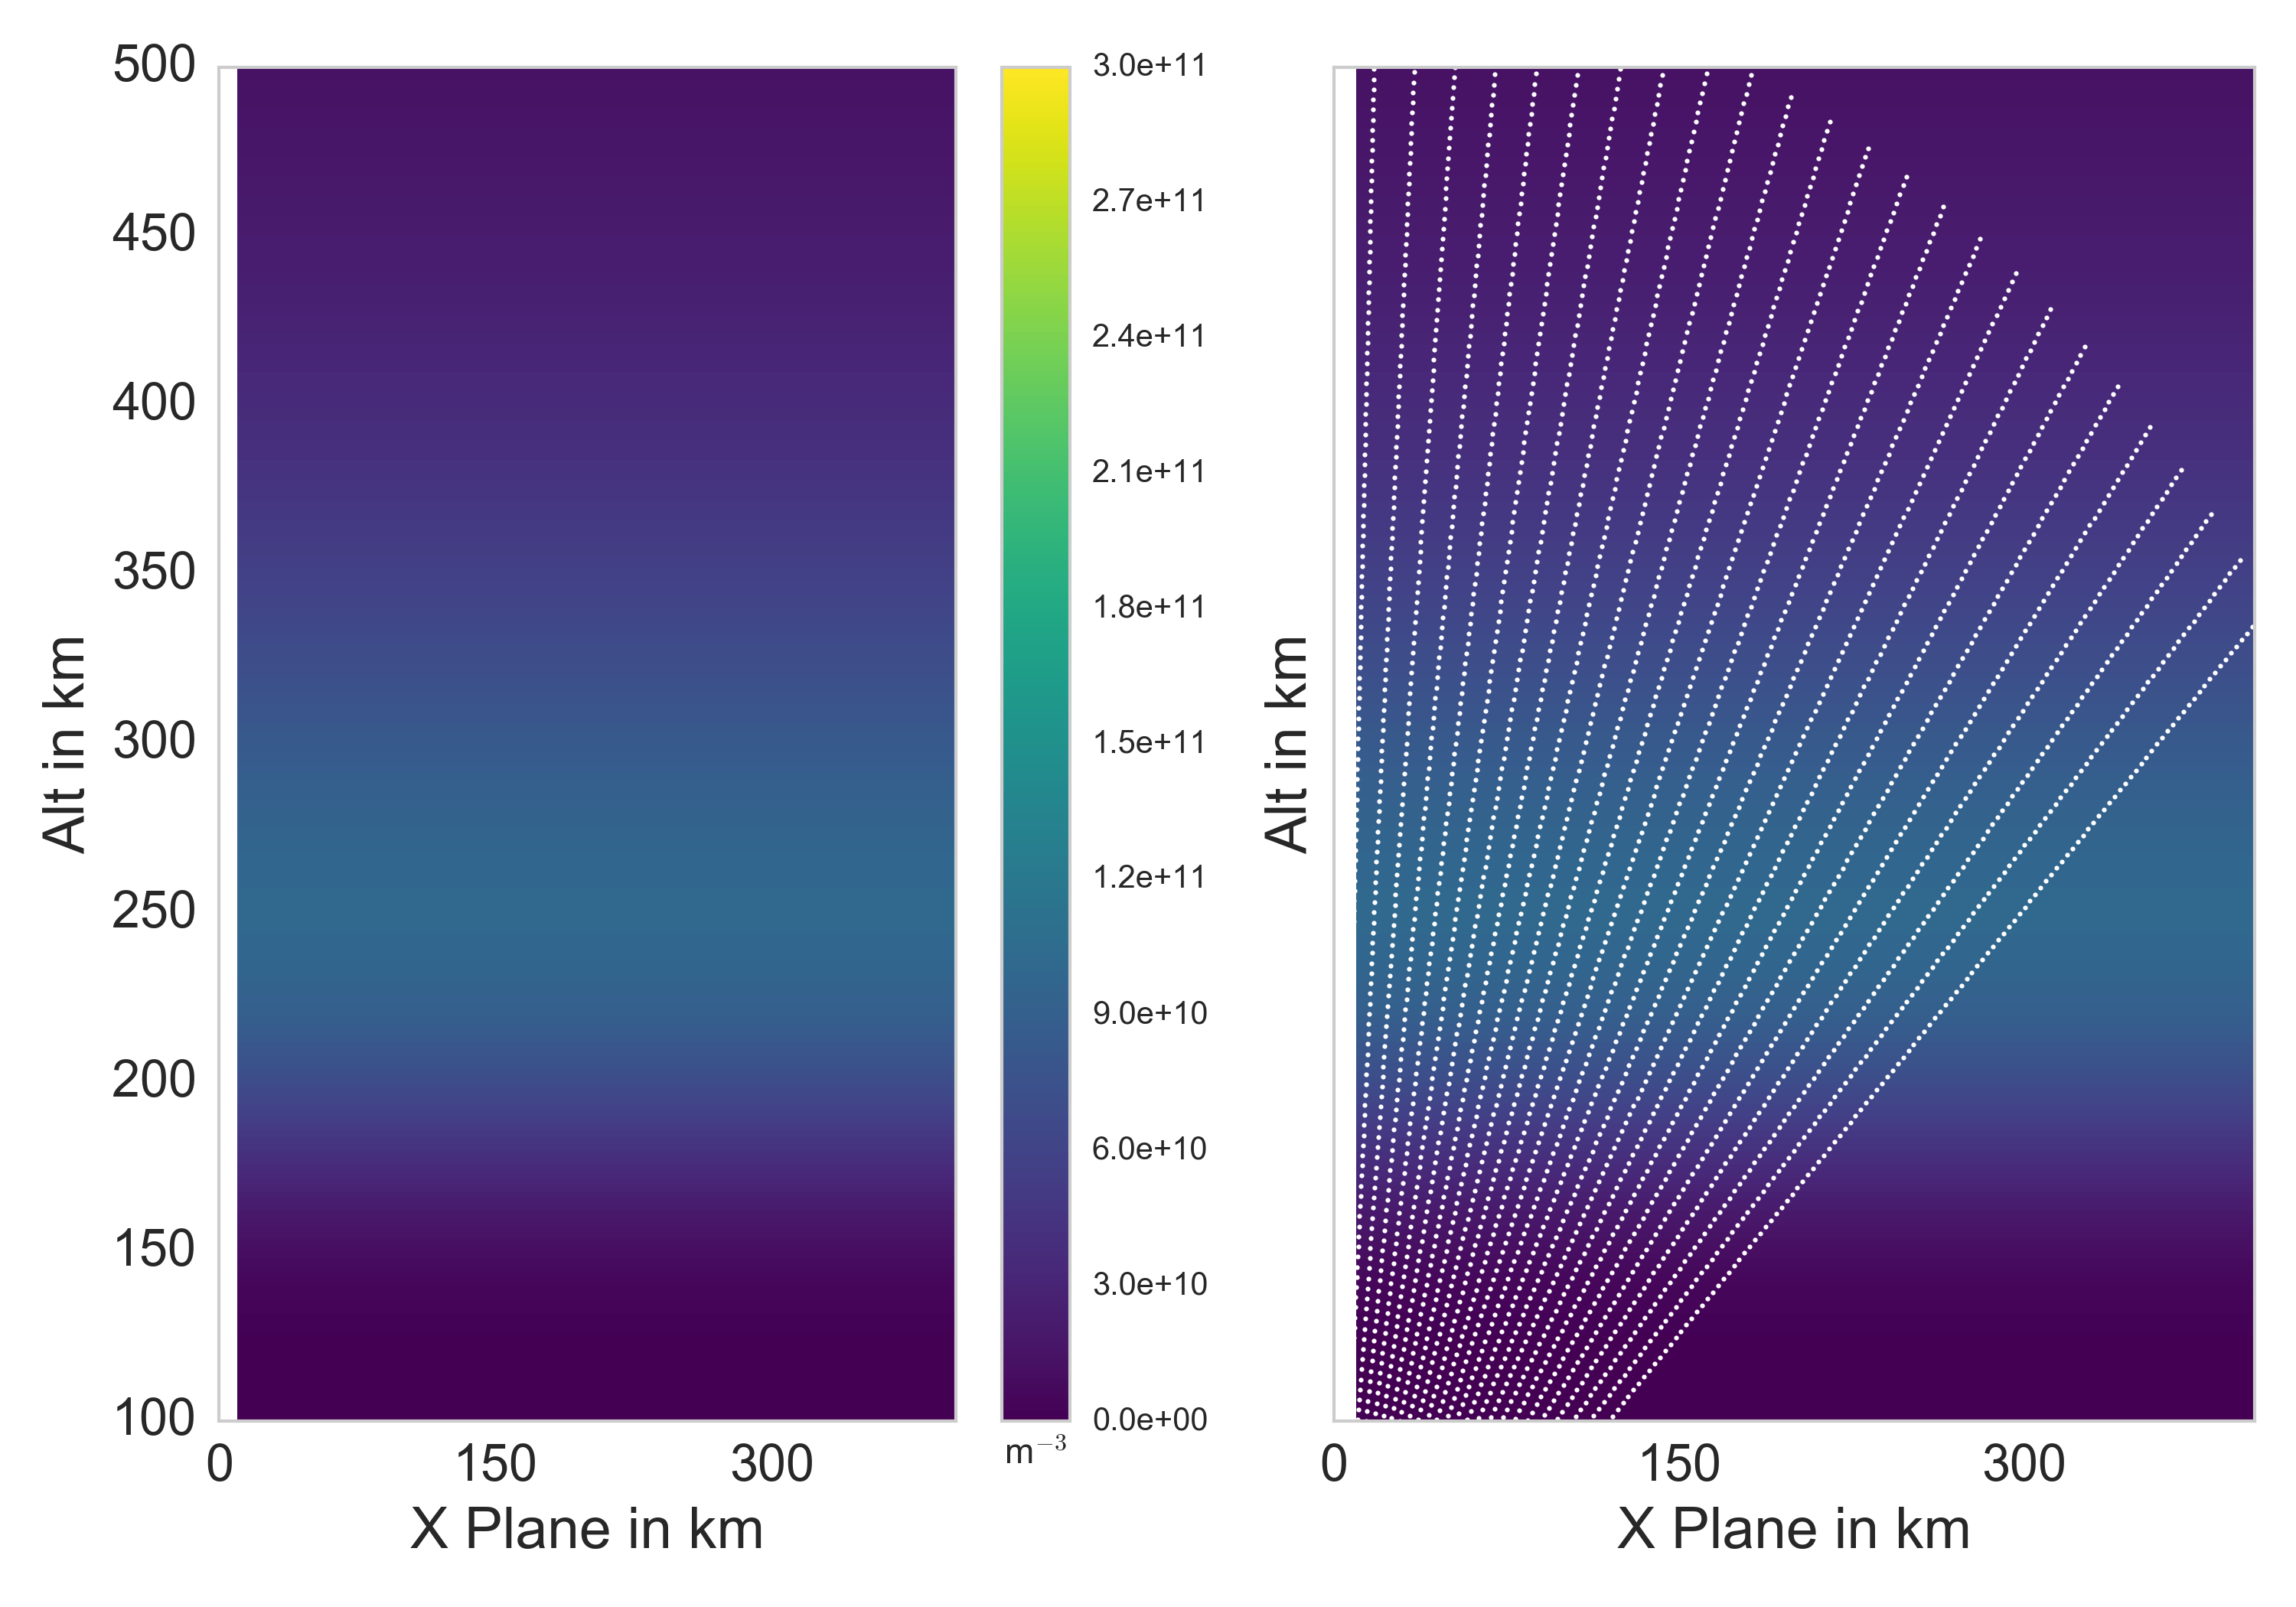
\includegraphics[width=3.5in]{backgroundandsamp}
\caption{Contour of background $N_e$ for simulations and the spatial sampling pattern}
% JOHN:  you don't need both of these panels, just the one on the right along with the colorbar.   Also, you should reduce the number of labels on colorbar, increase the font, and absorb exponent into units (which are not given).  Also there is no indication of what scalar is being plotted.   Typically you would write parameter/units above the colorbar:   $N_e (10^{10}$m$^{-3})$.   This comment goes for other plots too.
% Josh: I've updated the figures as you suggested.
% MZ - why run the colorbar out to 30 instead of the max density (~1.5e11) for this field?  Maybe because you want to keep the same colorbar for all density plots?
\label{fig:background1}
\end{figure}

%For these simulations we want to show how ambiguities could arise when trying to image just simple electron density enhancements with the beam pattern shown in the right panel of Figure \ref{fig:background1},
We first explore how a thin stationary density enhancement is resolved with the radar beam pattern shown in Figure \ref{fig:background1}, where each dot is a range gate in one of the 25 beams used. In Figure~\ref{fig:stationaryall}a, a thin density enhancement 2 km in width and 5 times the background is placed in the radar field of view. The enhancement is at the resolution limit of the original Cartesian grid, a delta function in the x direction.  The fitted electron density results from our simulation, without any additional averaging beyond the processing described in Section \ref{sec:acf},
%JOHN:  I don't know what "results of a single realization of our simulation" means here.  Is this different than "results of our simulation"?
%Josh: No extra averaging of fitted parameters.
are seen in Figure \ref{fig:stationaryall}b and c using 15 and 60 second integration times, corresponding to 60 and 240 pulses per position, respectively. The different integration times show that, although the enhancement is blurred, the variance of the measurement impacts the quality of the reconstruction because of the inherent noise-like nature of of the signal. The expected errors for both of the reconstructions are shown in Figure \ref{fig:errorstationaryall}. As expected, the estimated errors show that uncertainties are larger for the case with fewer pulses (i.e. smaller ensemble average size). 
%JOHN:  I've tried to fix figure referencing in the above since it didn't mesh with what you had.   Also, how are you deriving density, is it just range corrected power here, or full spectrum fitting?  
%Josh: Fitted density, I mention it in the previous paragraph
Because we know the input parameters, we can do a quick comparison using the root mean squared error (RMSE) for each case. By comparing the RMSE between the 15 and 60 second integration cases, we find that the ratio between the two cases is approximately 5.4 in the simulation output.  However, the expected RMSE ratio between the two should be approximately 2 since the variance of the ACFs scales as $1/\sqrt{J}$, where $J$ is the number of pulses. If we instead use a median instead of a mean operator in the error calculation, this ratio becomes 1.55, more in line with the expected statistical error scaling, largely due to the large outliers being disregarded.  Further investigation of the quantitative error discrepancy is a larger effort and beyond the scope of this study.  However, in general, the ratios between the errors and expected errors are relatively close when employing a median estimator that inherently rejects large outliers.
%% PJE: You've left me hanging here though - what does this result mean?  It deserves at least one sentence worth of comment.
%% JPS: Commented further, the behavior of the expected errors and actual errors are relatively close
\begin{figure}[!t]
\centering
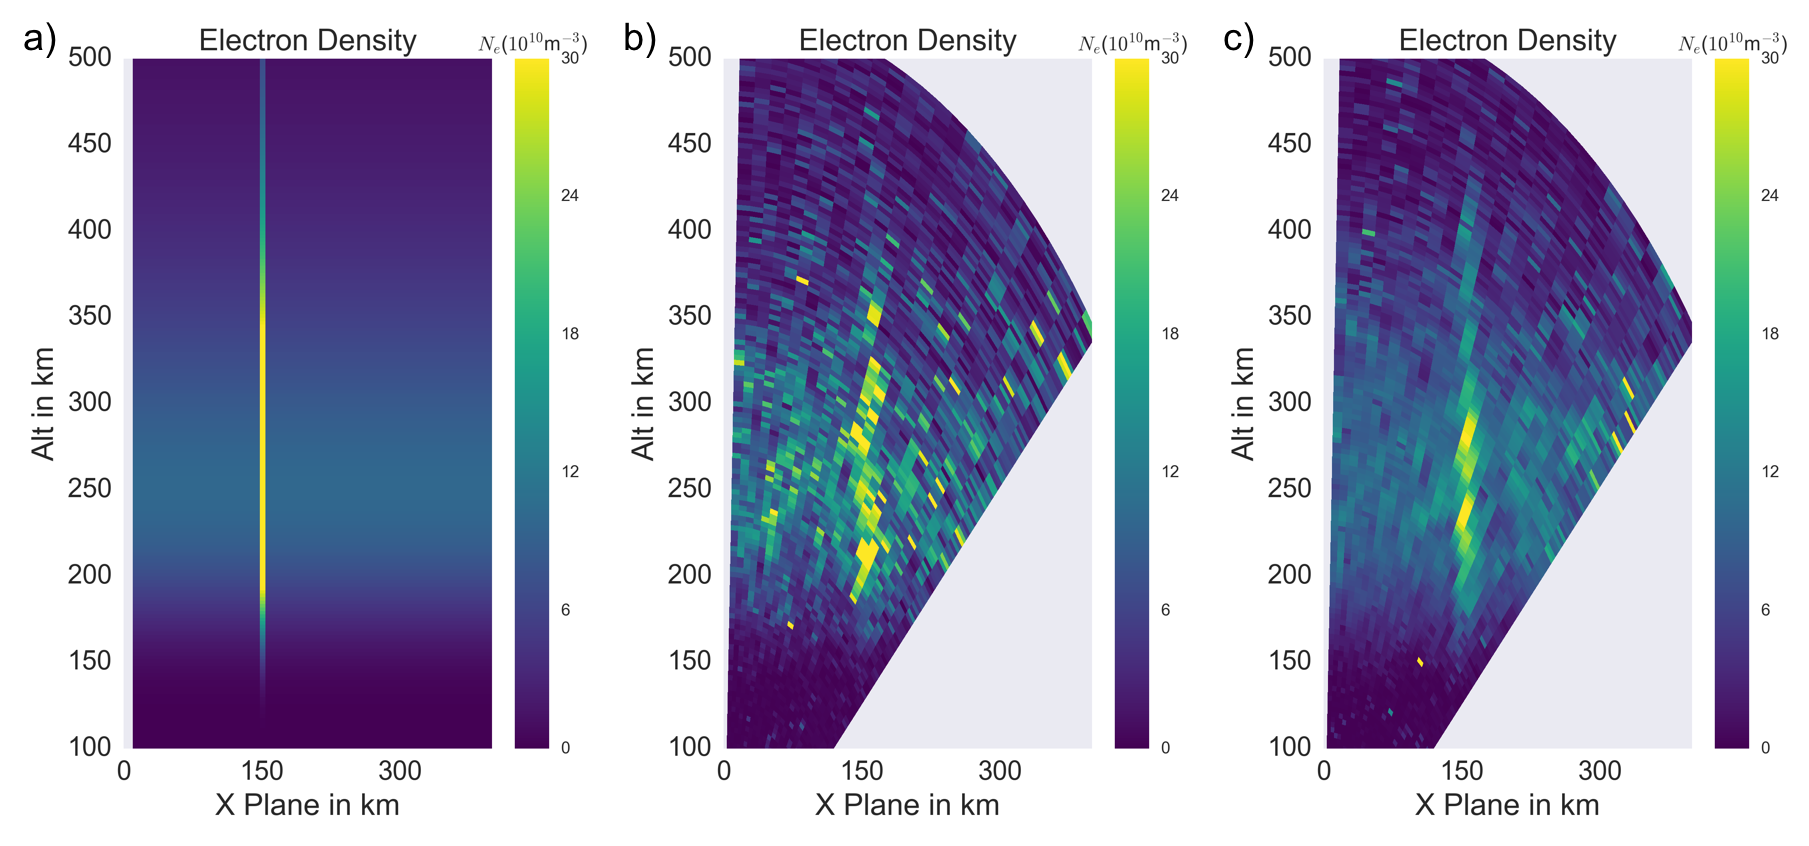
\includegraphics[width=6in]{stationary}
\caption{Results of stationary enhancement simulation. a) Input $N_e$. b) Output of simulator with 15 second integration. c) Output of simulator with 60 second integration.}
\label{fig:stationaryall}
\end{figure}

\begin{figure}[!t]
\centering
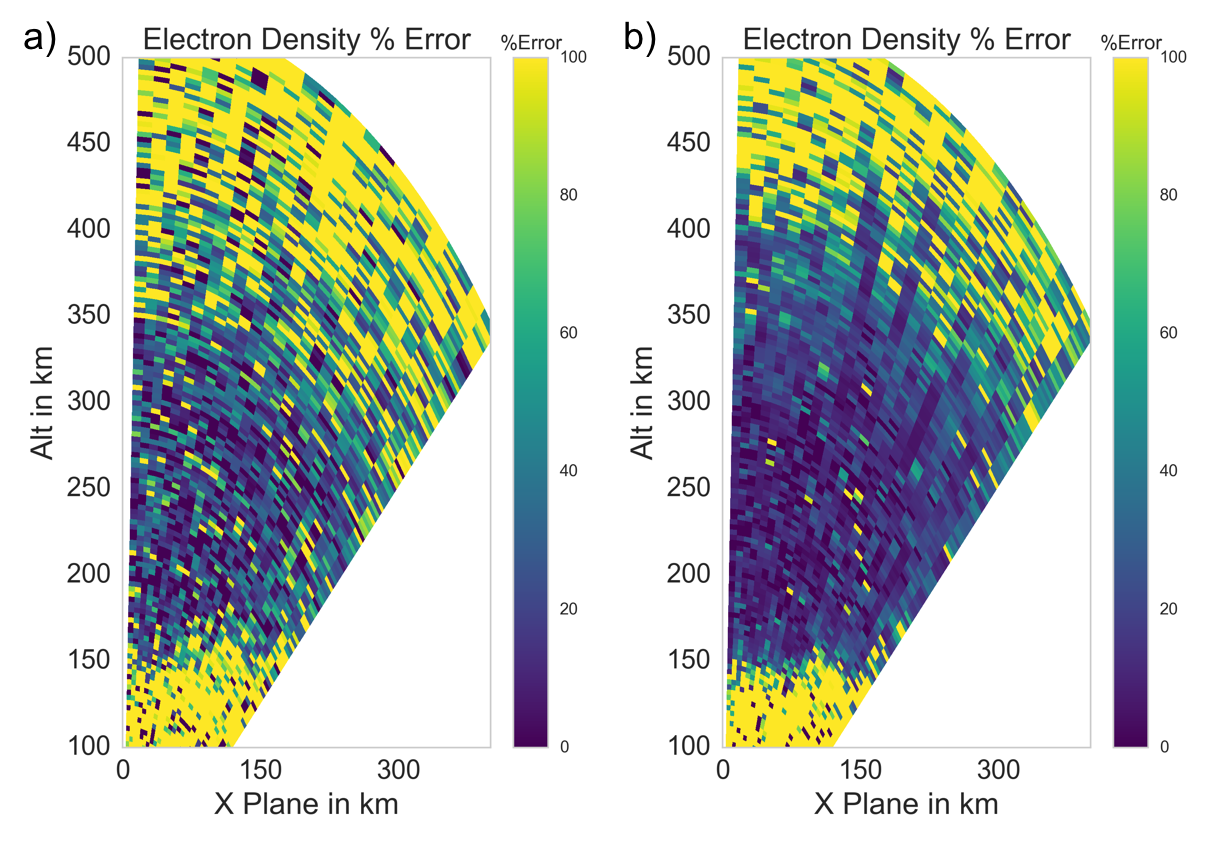
\includegraphics[width=4in]{Errorstationary}
\caption{Standard deviations from Figure \ref{fig:stationaryall}. a)  Estimate from fit for 15 second integration example. b) Estimate from fit for 60 second integration example.}
\label{fig:errorstationaryall}
\end{figure}

The blurring effect seen in this case study is not constant throughout the simulated space due to the way the radar samples the space. This is illustrated in Figures \ref{fig:moving10mins} and \ref{fig:moving14mins}, where as the enhancement moves through the scene at 500 m/s, its apparent size is affected by the orientation of the radar beams. 
%% PJE: please state the motion speed used
%% JPS: Done
As the enhancement becomes parallel to the radar beams, close to 0 km in the X plane,
%% PJE: where does it become parallel?  I cannot see the effect you are talking about here without some circles or arrows or something on the plot.
%% JPS: Done
%% JLS:  Actually the effect is more nuanced than just becoming thinner.   The density column is bifurcated below 200 km (two columns with gap in between).   DO you know why this is?  Is it a consequence of the shape of the ambiguity function, such that the target "fades" as it moves across beams?
its morphology in the reconstruction becomes smaller along the X-axis, as the range ambiguity is much larger than the cross range ambiguity. In both cases the expected errors, shown in panel c in both Figures \ref{fig:moving10mins} and \ref{fig:moving14mins}, give us confidence in these results as they are much lower value than the enhancements and background.
%% PJE: the electron density error plots here have the wrong scaling - everything is very dark color and I can't see any structure in any of them.  Please rescale the color bars.
%% JPS: added statement about errors
%% JLS: Hard to read the scales, but looks like you are using the same range for data and error.  The saturated error pixels don't matter, so why not compress the range so reader can visualize error in vicinity of the features we are trying to reconstruct?
\begin{figure}[!t]
\centering
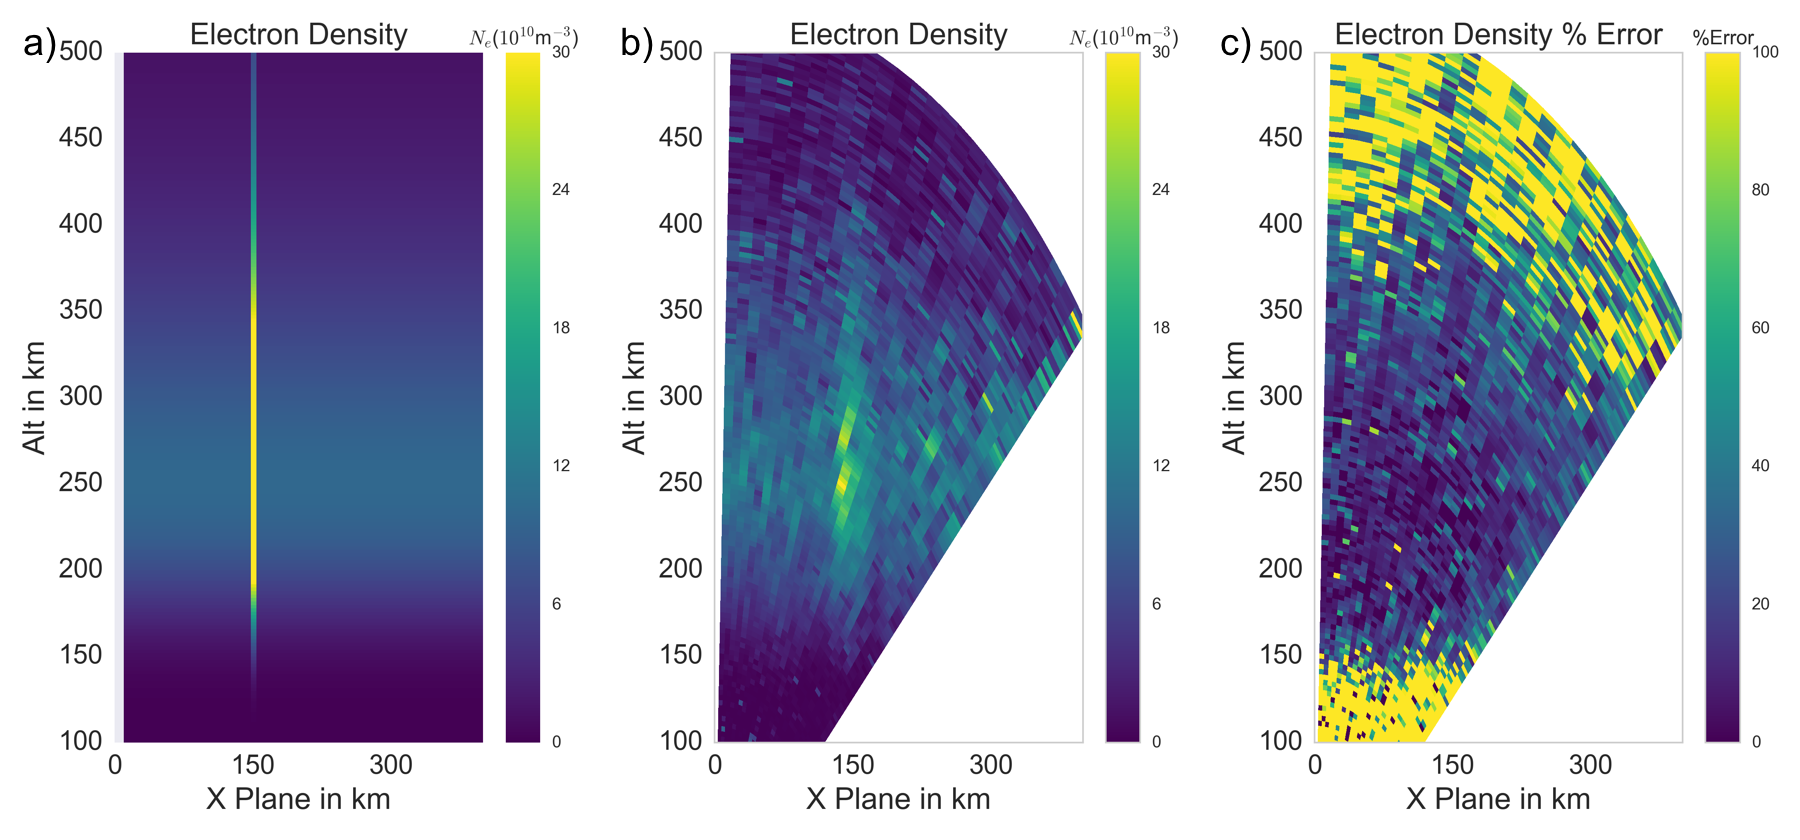
\includegraphics[width=6in]{moving6mins}
\caption{Results of moving enhancement simulation at 600 seconds. a) Input $N_e$. b) Output of simulator with 60 second integration. c) Estimated errors from fit.}
\label{fig:moving10mins}
\end{figure}


\begin{figure}[!t]
\centering
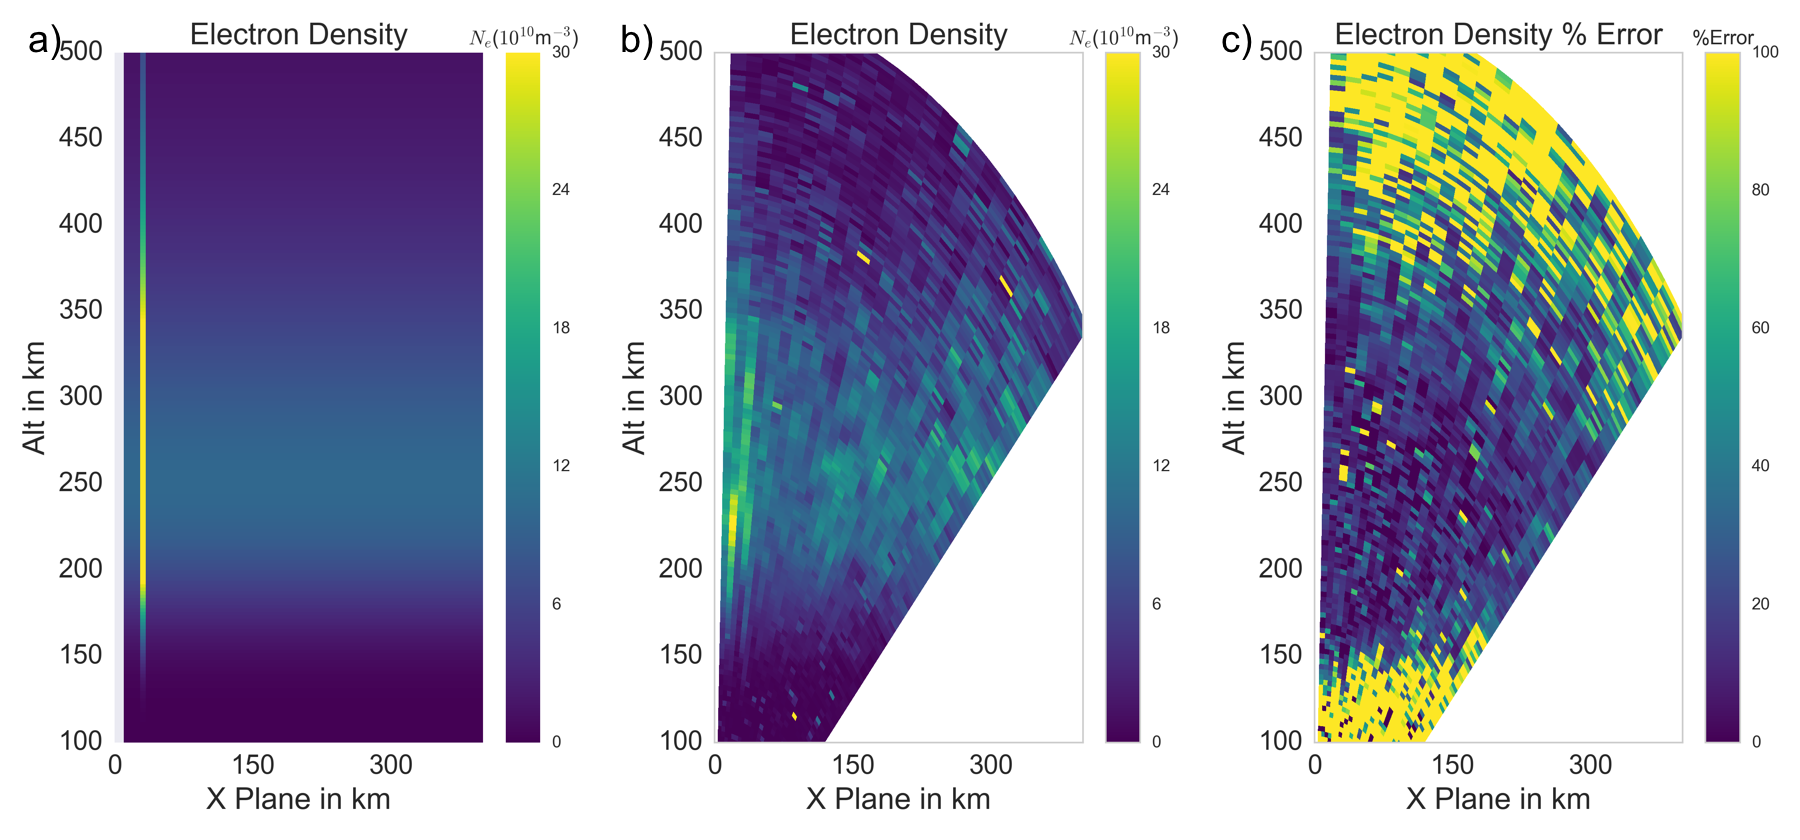
\includegraphics[width=6in]{moving14mins}
\caption{Results of moving enhancement simulation at 840 seconds. a) Input $N_e$. b) Output of simulator with 60 second integration. c) Estimated errors from fit.}
\label{fig:moving14mins}
\end{figure}

This change in the shape of the enhancement can give the impression that its morphology has evolved as it was moving through the field of view of the radar. This could lead to an incorrect interpretation of the physical process taking place, and issue raised by \cite{Dahlgren:2012dq}.   Thus, one must be careful when analyzing these sorts of reconstructions.

Lastly, for this type of simulation, we show an example to demonstrate the situation where a set of two different input parameters can yield qualitatively similar results. For these cases we create electron density enhancements similar to those seen in the high latitude observational study of \cite{Semeter:2005fo} during a poleward boundary intensification event. The sizes of these enhancements are 10 km width and 18 km width. The enhancement in the 10 km width example is 6 times higher than the background while the 18 km width enhancement is 3 times higher than the background.

The input electron density, the fitted electron density and the expected error for the 10 km enhancement can be seen in Figure \ref{fig:moving10all}. The same images for the 18 km wide case can be seen in Figure \ref{fig:moving18all}. Both cases show that electron density enhancements are well above the expected errors.
%% PJE: once again, I cannot see the error morphology here - it just looks like a bunch of pixels at the lowest color level.  Rescale.
%% JPS: I think showing the errors in the same color scale gives the reader an easier time of determining if the results should be trusted. 
%% JLS:  Fine, but all the reader can say from these plots is that the error seems to be below ~12, or ~30%.   DIfficult to discern any color differences below that.
The fitted electron density for both the 10 km enhancement and 18 km enhancement cases show nearly identical results. This simple example demonstrates the possibility to create a non-unique solution in ISR experiments. The results further demonstrate that SimISR can provide useful information in this case, in that it can provide information during the design phase of an experiment that highlight possibilities for ambiguous observational results between two different sets of phenomena. 

\begin{figure}[!t]
\centering
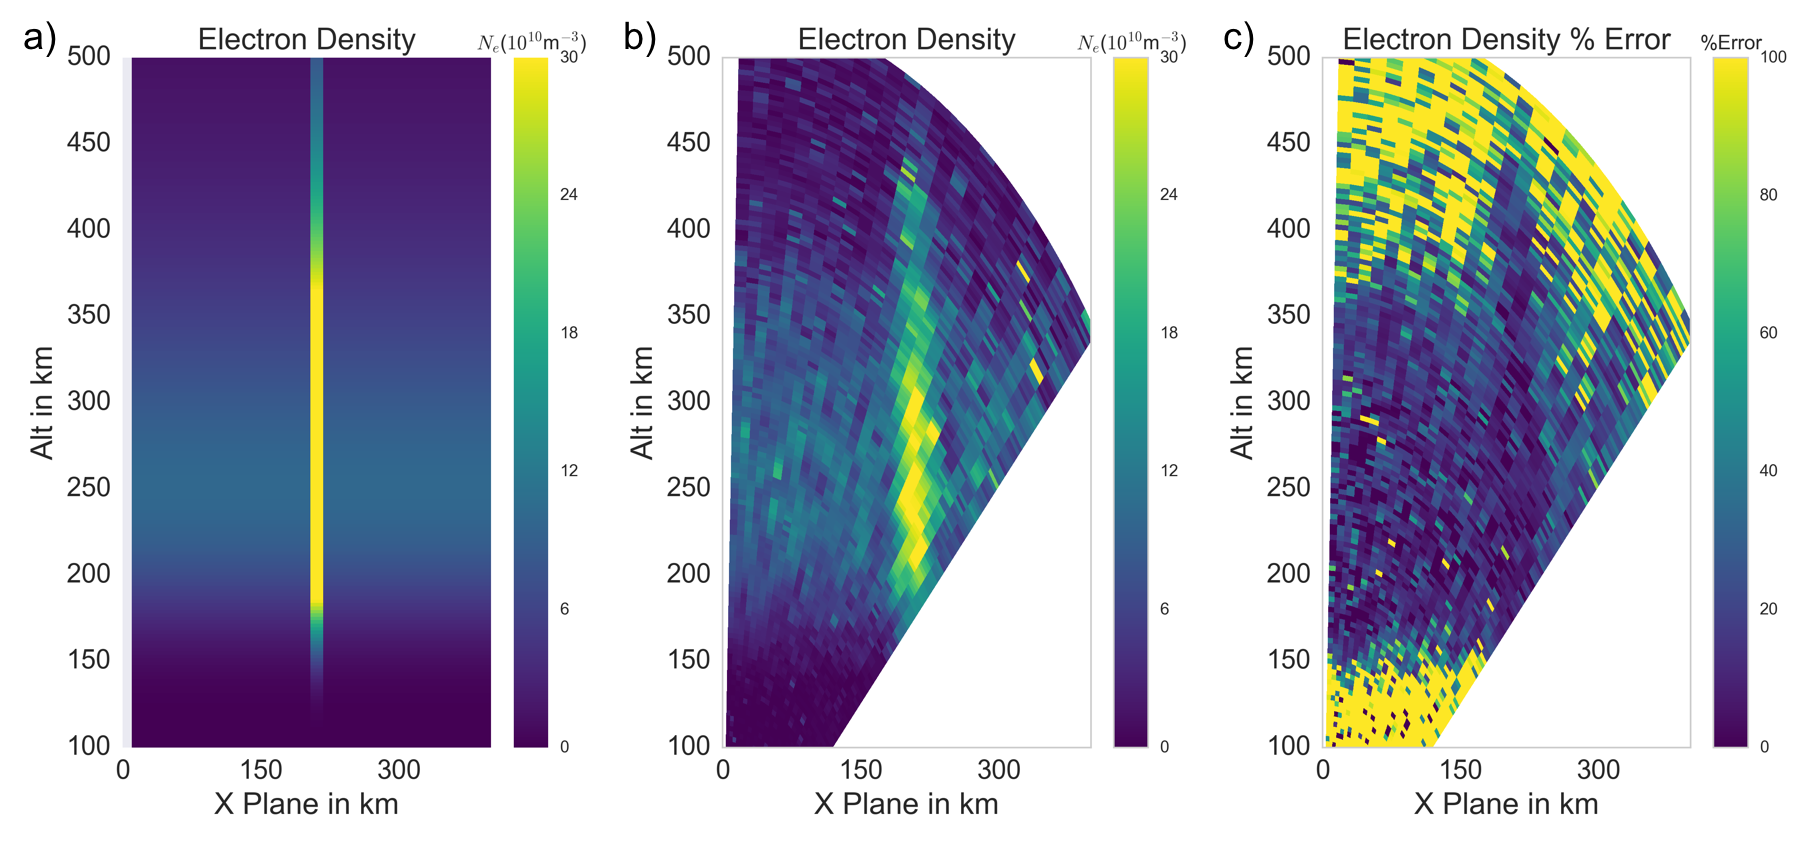
\includegraphics[width=6in]{moving10kminouterr}
\caption{10 km wide enhancement moving simulation at 480 seconds. a) Input $N_e$. a)  b) Fitted $N_e$ with 60 second integration. c) Estimated error from fit.}
\label{fig:moving10all}
\end{figure}

\begin{figure}[!t]
\centering
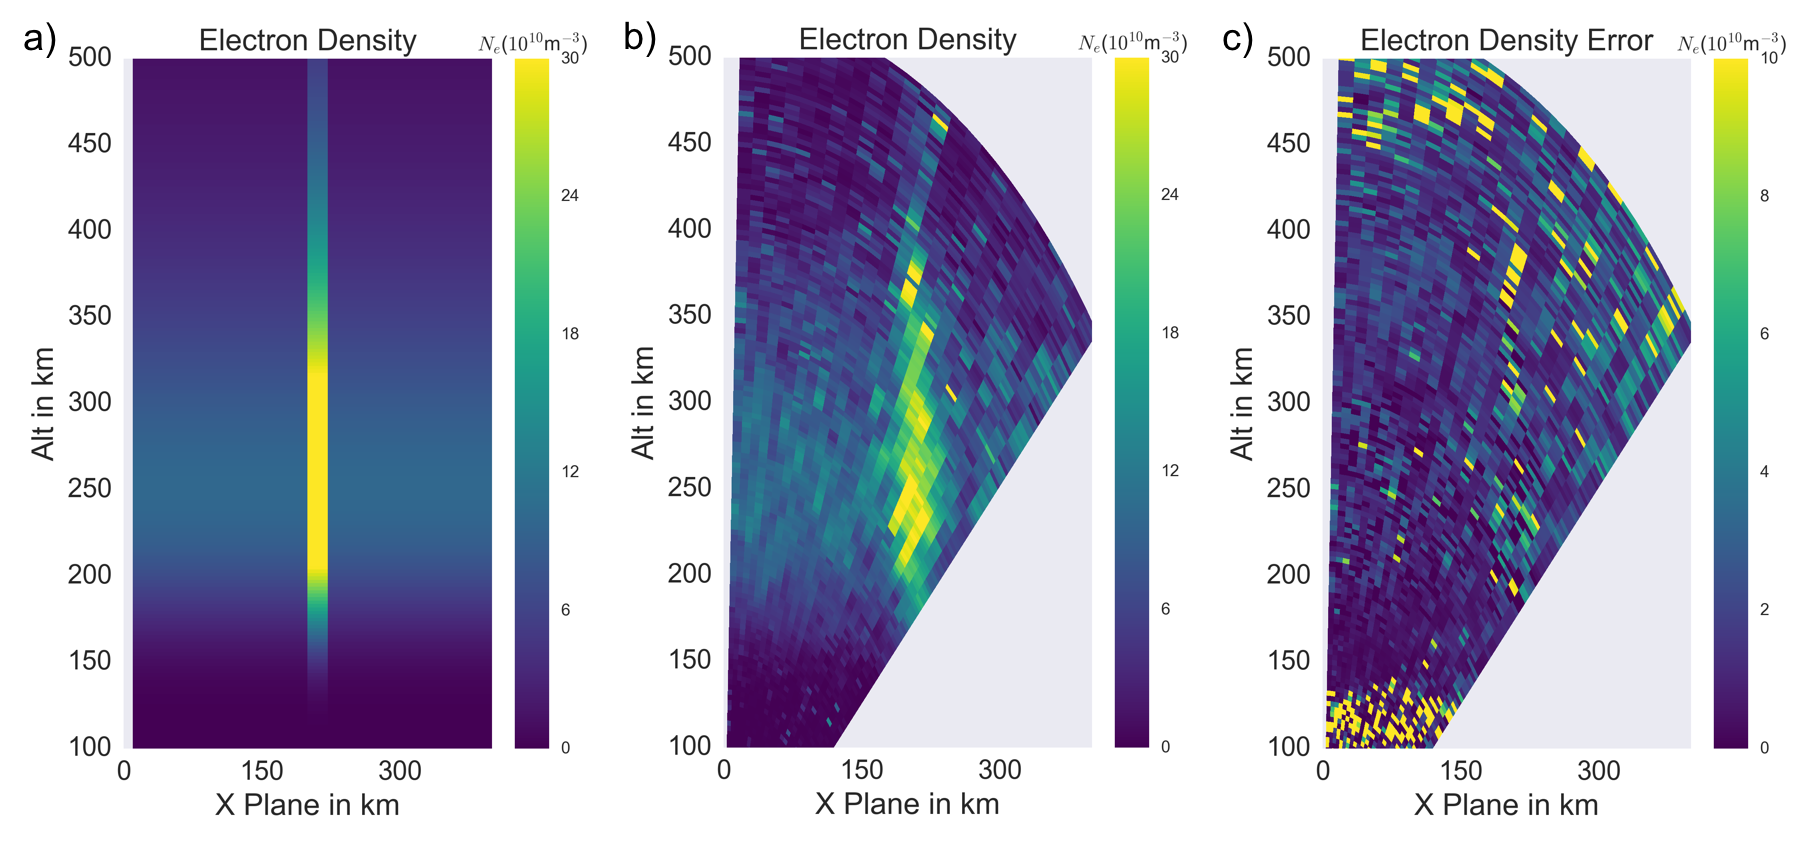
\includegraphics[width=6in]{moving18kminouterr}
\caption{18 km wide enhancement moving simulation at 480 seconds. a) Input $N_e$. a)  b) Fitted $N_e$ with 60 second integration. c) Estimated error from fit.}
\label{fig:moving18all}
\end{figure}

\subsection{Full Parameter Experiment}
\label{sec:fullparam}
Another SimISR use case employs input plasma parameters derived from the multi-fluid model developed by \cite{semeter:plasmatransport2012}. The specific model run was originally used by \cite{Perry:2015jf} to assist in interpreting measurements of polar cap arcs from the Resolute Bay Incoherent Scatter Radar (RISR). Images of the modeled plasma parameters are shown in Figures \ref{fig:plparamst0} and \ref{fig:plparamst60}. The enhancements in electron density, electron temperature, and ion temperature comprise the self-consistent response of the ionosphere to a field-aligned current system with amplitude .875 $\mu$A/m$^2$.  The source is made to move with respect to the radar at a velocity of 200 m/s (a  value inferred from optical forms observed during this event).  A channel of soft electron precipitation (50-500 eV in energy) is added to the upward current channel, with energy flux consistent with the amount of electron heating seen during the event.  A reasonable objective for a multi-beam ISR experiment could be to validate model predictions of conditions leading to the arc-adjacent density depletion seen in panel a of Figure \ref{fig:plparamst60}.  In this specific case SimISR can be used to assess observability of dynamic plasma structuring and establish confidence intervals on the ISR results.  

%MZ - something looks strange in this figure with Ti - is the a species-averaged or composition-corrected value?  Also I would strongly recommend removing N2+ from this figure, since it doesn't matter at all in this event (viz. it is at least 1000 x lower density than dominant species at all alts.).
\begin{figure}[!t]
\centering
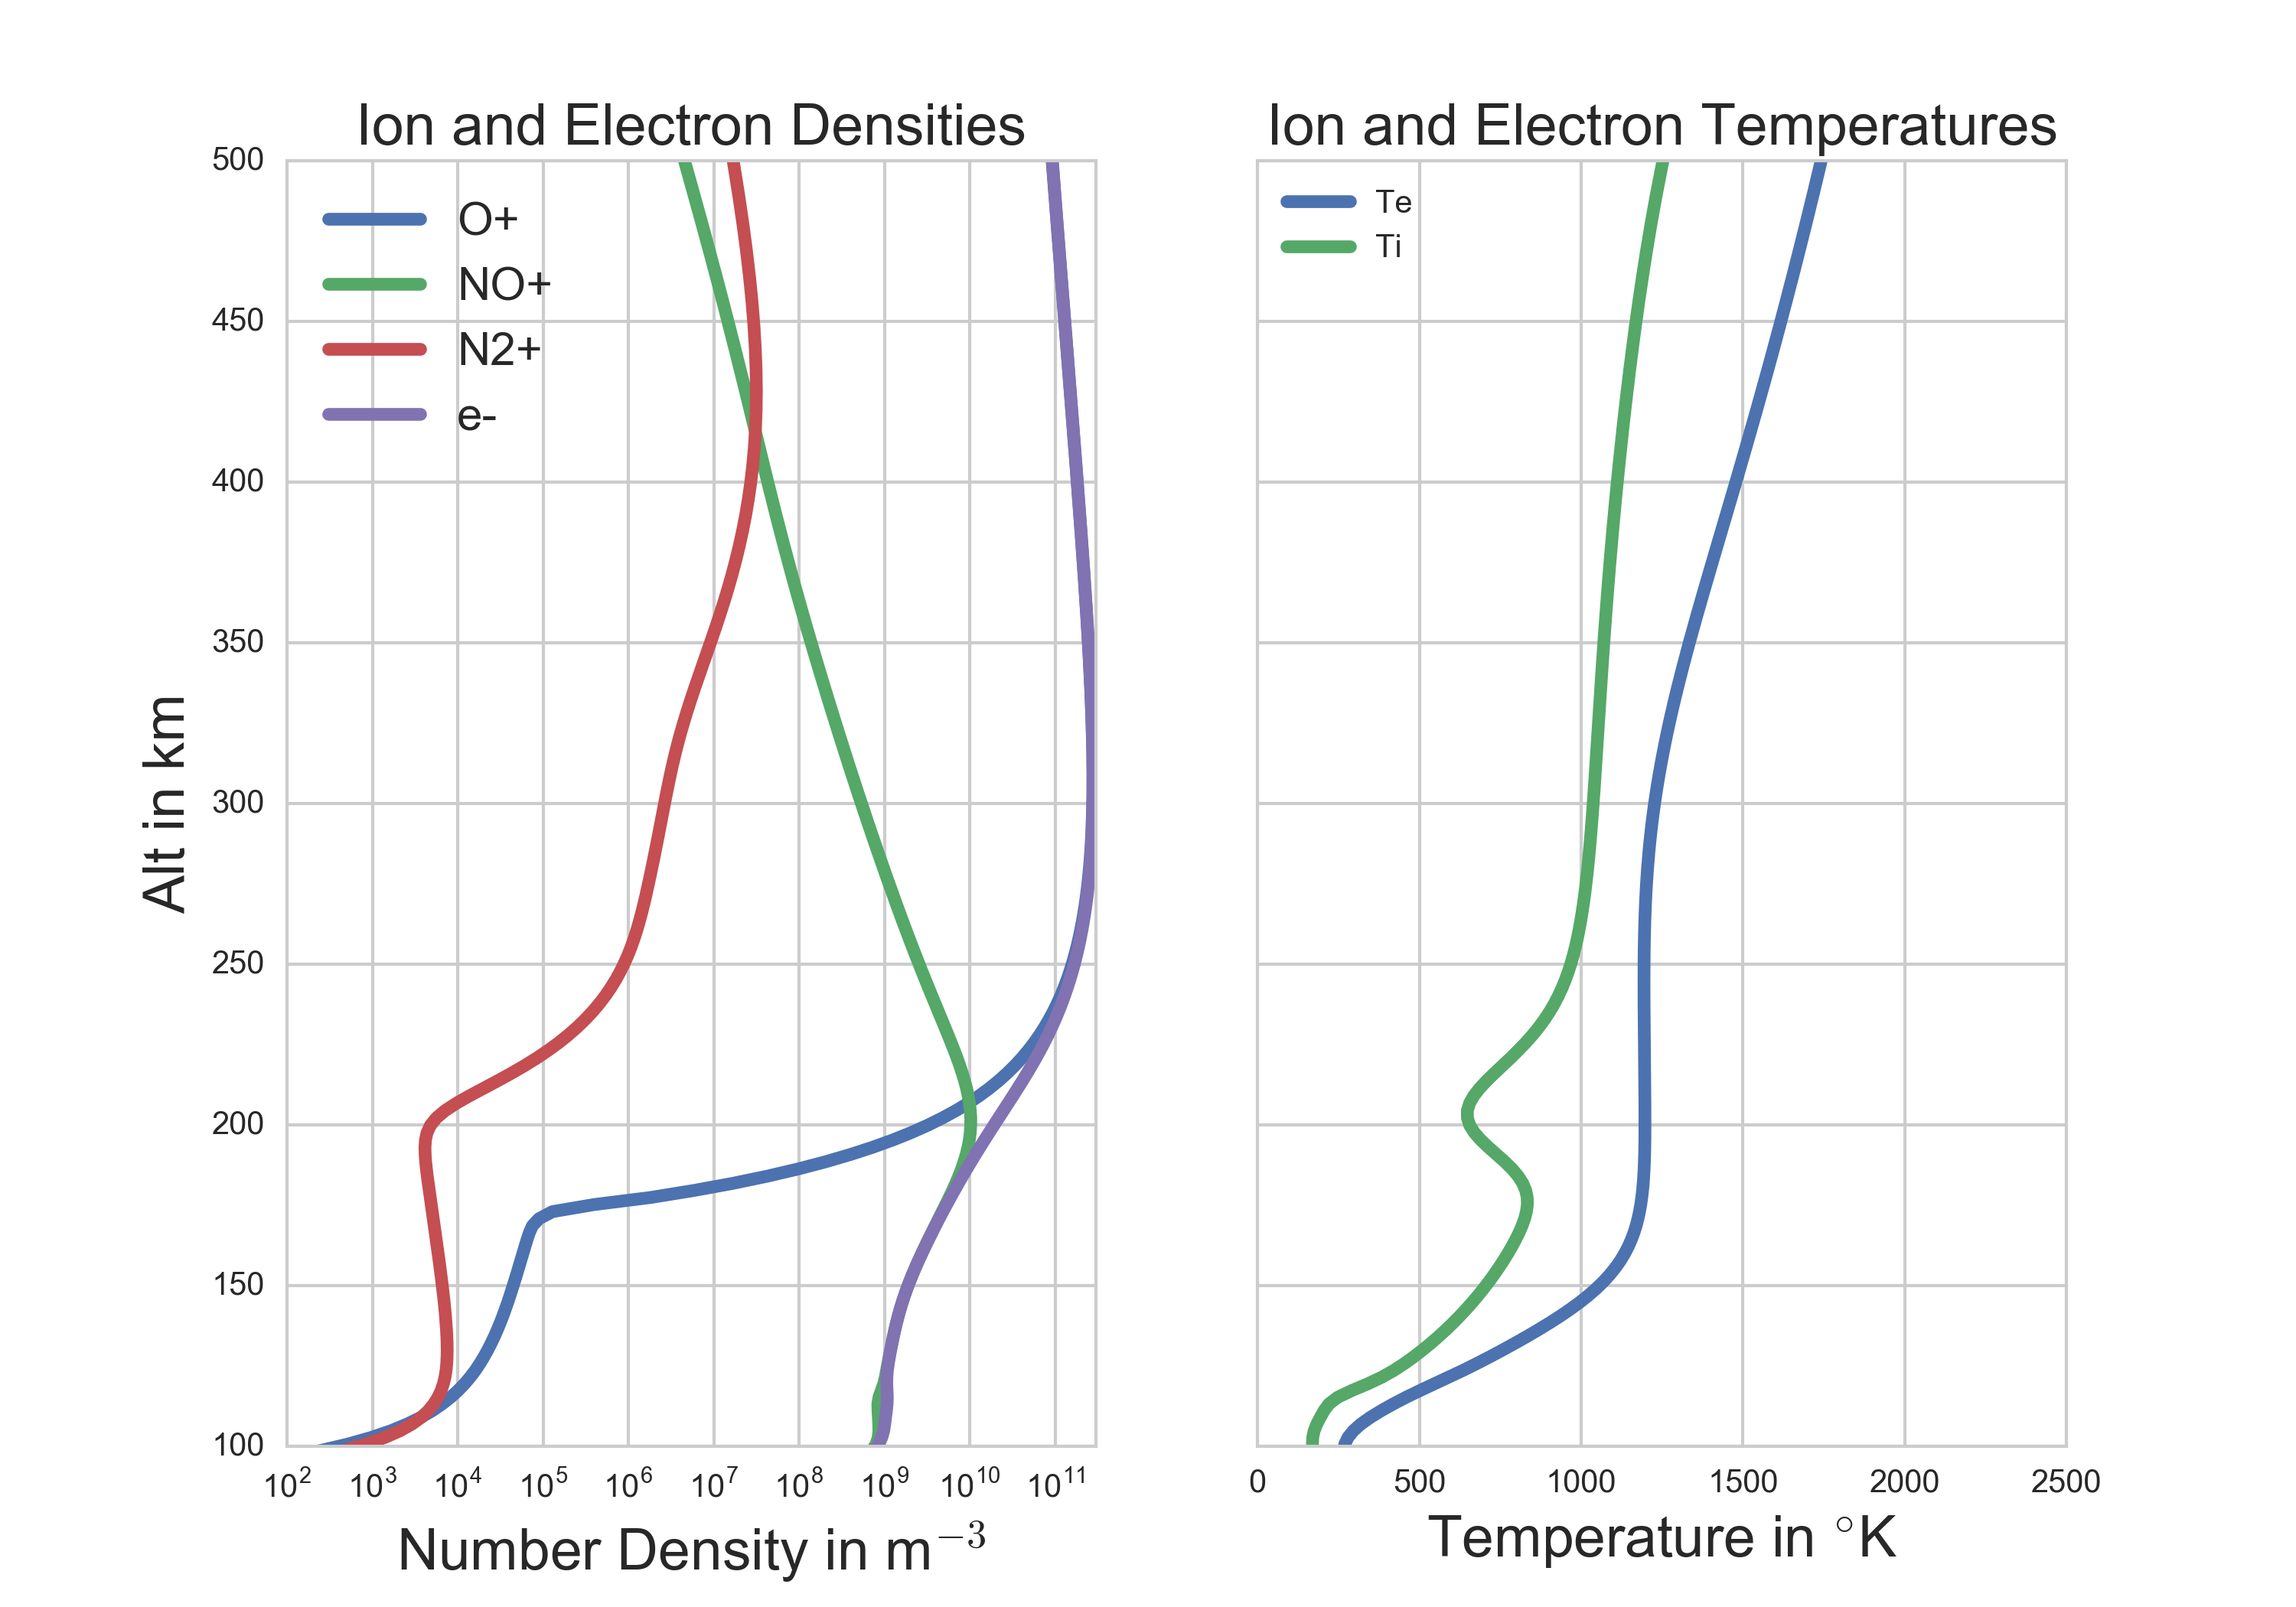
\includegraphics[width=6in]{backgroundallparams}
\caption{Background ionospheric parameters ($N_e$, $T_e$, $T_i$) along with number density of ion species, used for simulations.}
\label{fig:plparamst0}
\end{figure}

%MZ - K or deg. K?  Back in the day they taught us to just use "K", but maybe that has changed...
\begin{figure}[!t]
\centering
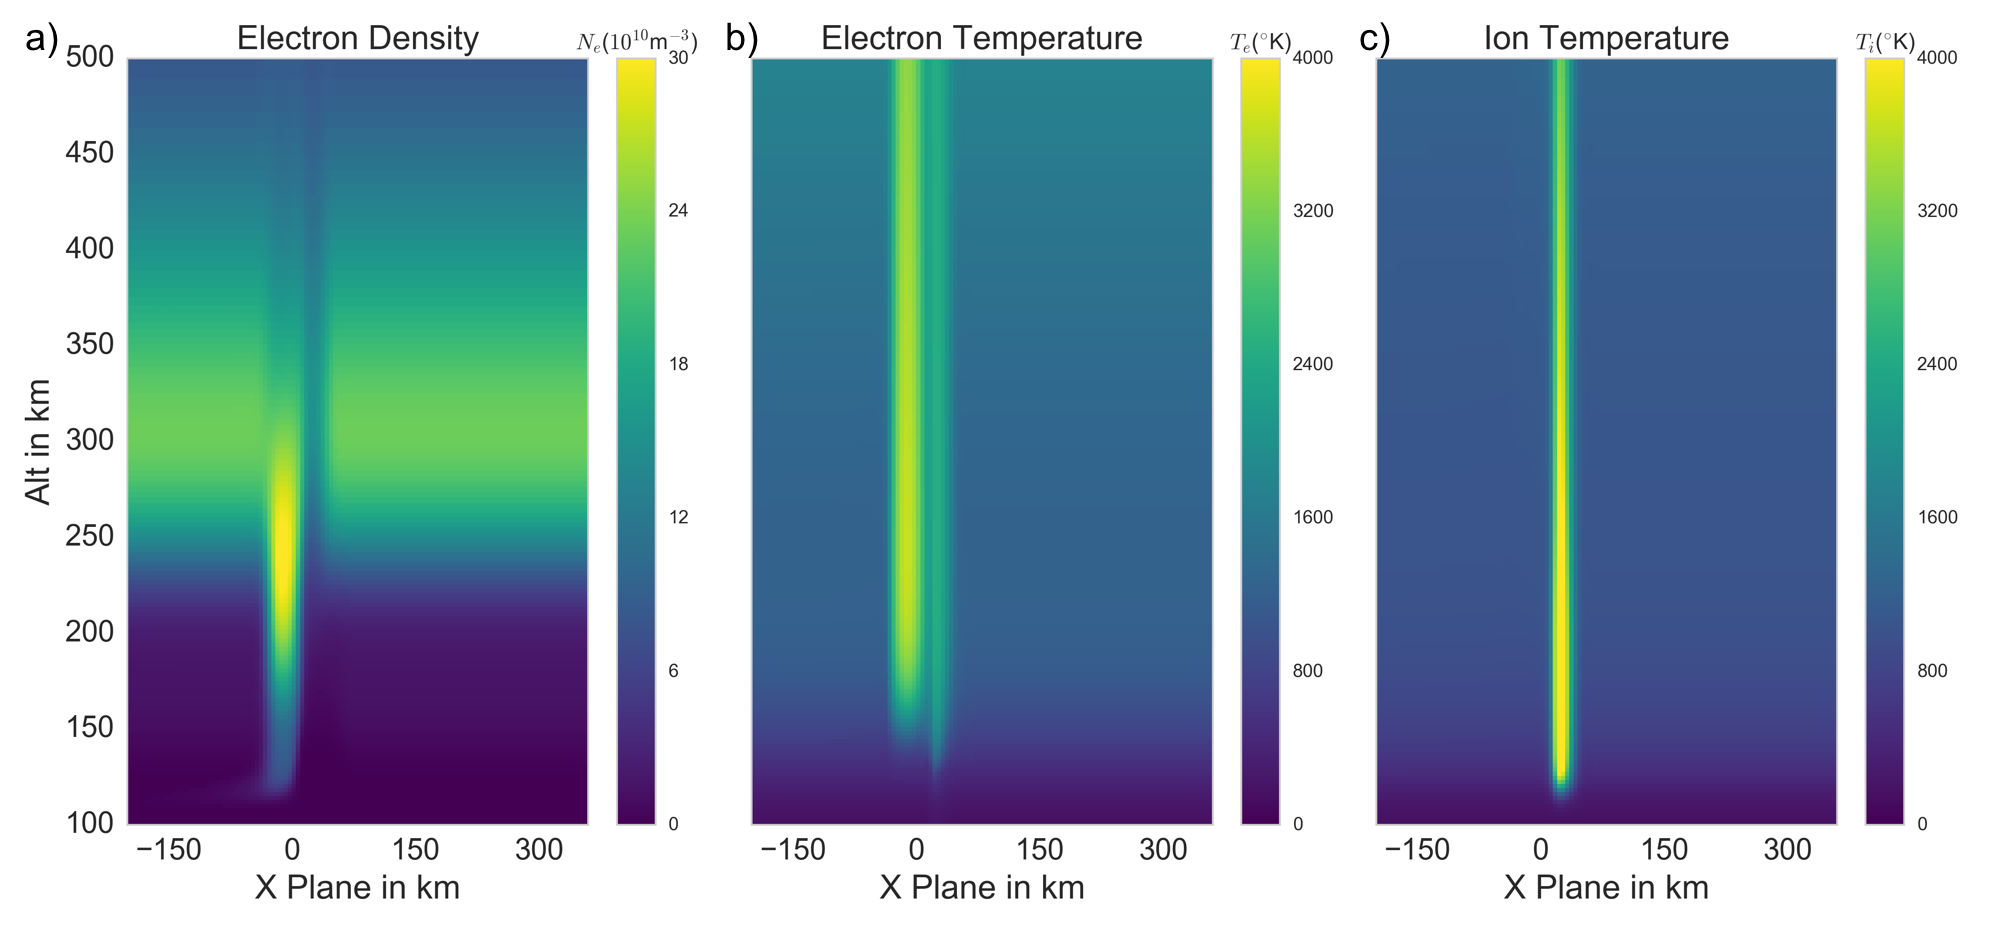
\includegraphics[width=6in]{0960_15_int}
\caption{Perturbations to Figure \ref{fig:plparamst0} due to an imposed current system of .875 $\mu$A/m$^2$ at $t=960$ s, representing an polar cap auroral arc which is sweeping across the field-of-view of the radar at about 200 m/s \cite{Perry:2015jf}.}
\label{fig:plparamst60}
\end{figure}

Using a beam pattern similar to the one seen in the right panel of Figure \ref{fig:background1}, we use SimISR to explore how an electronically scanned ISR may reconstruct this dynamic auroral arc system.  For the purposes of illustration, we use the contrived case where the radar spatial beam pattern is defined to be in the plane of convection.  It is also assumed that the ion species present (particularly their individual masses and relative concentrations) are known. This is a common use case in ISR fitting, as allowing ion concentrations to be free parameters can in some situations allow for non-unique solutions depending on the ion species that are present.  If the fixed, a priori composition ratios between the different ion species are incorrect, this can lead to errors in the final parameter estimates, with ion temperature particularly affected. For the lower F region ionosphere, parameter distortions can occur between 150-250 km where the ionosphere changes from NO$^+$ dominated to O$^+$ dominated \cite{Zettergren:2011ej,Blelly:2010gf}. We also note that as the field aligned current passes through the simulated field, an influx of NO$^+$ appears in the region of rapid ion mass transition for this simulation, potentially violating ion composition assumptions \cite{Perry:2015jf}.
% JOHN:  I can't figure out what the above sentence fragment is supposed to be.
% Josh: I fixed the first sentence of the previous paragraph
% MZ - I'm intrigued by the last sentence.  We do need to explain this a bit better (and I would like to go through the model output from which this is derived to make sure I understand why the model it giving this result)

The output of SimISR in the auroral arc case can be seen in Figure \ref{fig:fplparamst60}. The integration is started at $t=960$ s into the multi-fluid simulation with the plasma parameters shown in Figure \ref{fig:plparamst60}. For this case, a 60 second integration time is used, which for the 27 beam radar experiment set up gives 255 pulses per position. These plasma parameters are linearly interpolated to a Cartesian grid and plotted using the GeoData API \cite{john_swoboda_2016_154533}. Lastly, the expected errors from the fit can be seen in Figure \ref{fig:fplparamst60err}, which are of much lower value that the fitted parameters.
%% PJE: same complaint about expected errors - I can't see anything with the color scale chosen.  Rescale.
%% JPS: See other comments.
We highlight several features in the fitted results. First, the predicted enhancements in electron and ion temperature are clearly observable and well above the expected error. Second, we examine whether the predicted density cavity in the downward field-aligned current region is  detectable. A deepening and broadening region of plasma evacuation is predicted as a self-consistent response to a confined up-down current pair \cite{cran;cavity}.  But it has been unclear whether this prediction can be validated with ISR, since it involves detecting organized channels of reduced backscatter power embedded within a higher density background.
%% PJE: I really don't like the word "coherent" here since it will lead the reader to think of scattering off coherent plasma waves.  I think you should use maybe "organized channels".
%% JPS: Done
%Josh: You didn't have the right citation so I found the best one i could Replaced \cite{write:alfven} with current version
% JOHN:  The Cran-McGreehan paper cited above is the right one, just check that it compiles.
% Josh: It seems to work on my end.
% MZ - I'd be careful attributing the cavities to the Cran/Doe Mechanism.  I think case I think it is a chemical effect (which is, I believe, what Perry et al, 2015 conclude).  However, in general, you would likely not be able to separate the two process with ISR measurements.  
The images shown in Figure \ref{fig:fplparamst60} represent the best case scenario for identifying the presence of this cavity since, at this time, the cavity is nearly co-aligned with one of the beams. 
%For the other cases where the beams are not well aligned with the cavity it becomes much more difficult to observe it due to the range ambiguity being larger than the beam width, making the "filling in" of the evacuated electrons more pronounced. 
Using density measurements alone (panel a) the presence of the cavity is visible, but only marginally so, as it is blended with the adjacent  enhancement produced by the applied precipitation in the upward current channel.  A similar ambiguity exists with the electron temperature result, which could easily be interpreted as purely an effect of heating from soft precipitation.   However, the ion temperature increase in panel b is decidedly narrower than the electron temperature enhancement, offering a possible observable fingerprint for the presence of a confined up-down current pair.  The simulation result illustrates the efficacy of a collective analysis of all plasma state parameters in evaluating the physical mechanism responsible for an observed dynamic.  This is a common approach in data assimilation problems.

%% Fitted Data

\begin{figure}[!t]
\centering
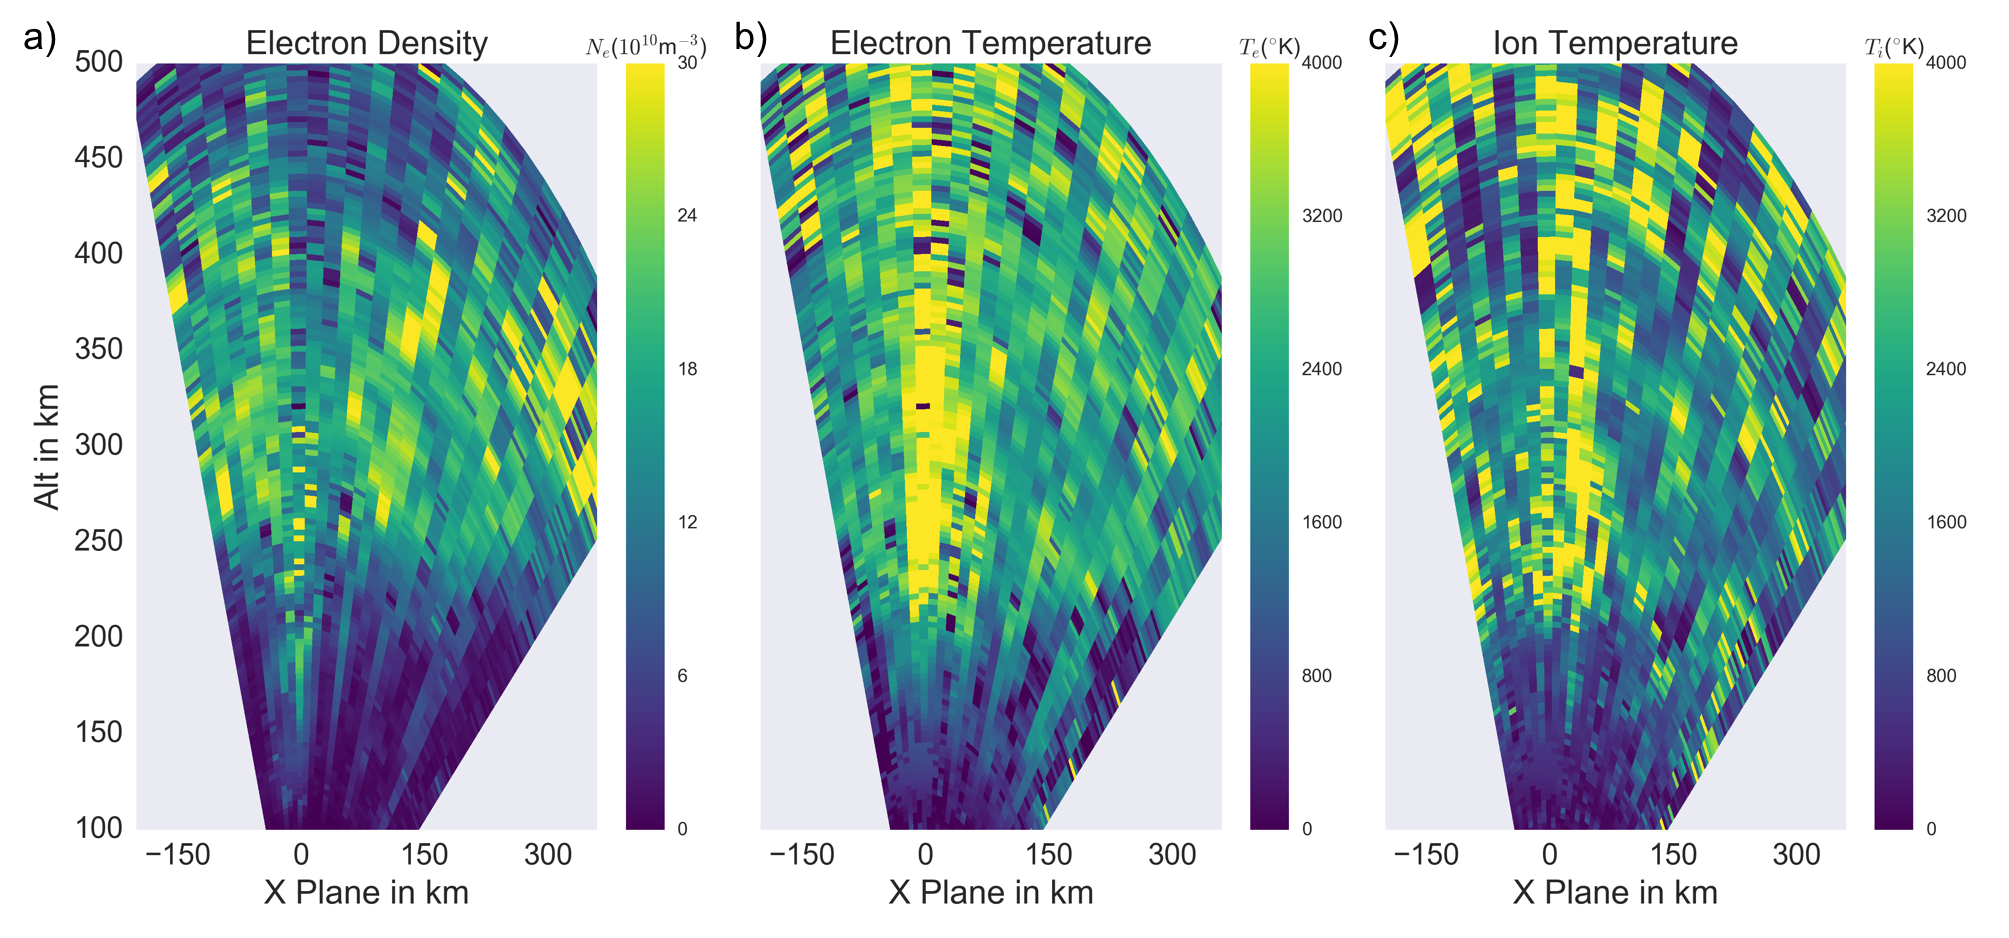
\includegraphics[width=6in]{0960_60_int}
\caption{Fitted Plasma Parameters for the auroral arc case at $t=960$ s with 60 second integration.}
%JOHN:  need to label these A,  B, C
%Josh: I have the parameter type in the title so that should be enough.
\label{fig:fplparamst60}
\end{figure}

\begin{figure}[!t]
\centering
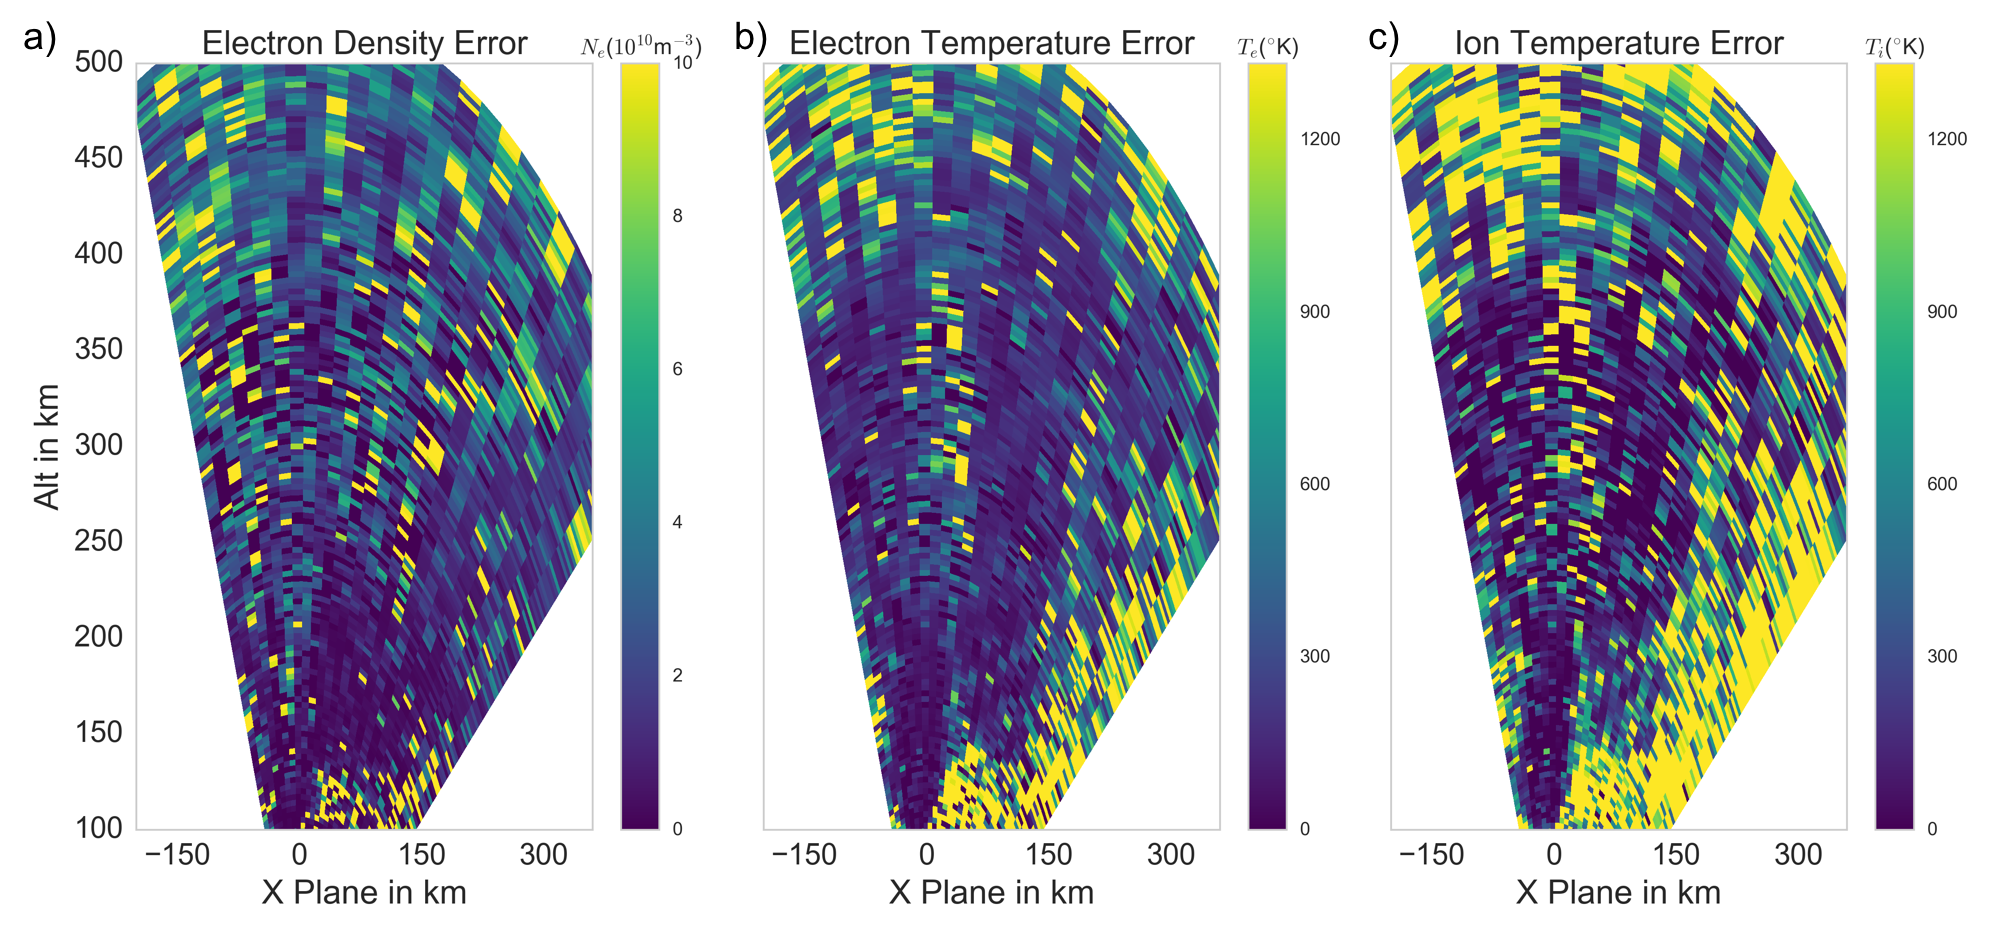
\includegraphics[width=6in]{0960_60_int_err}
\caption{Estimated errors from fitted Plasma Parameters for the auroral arc case at $t=960$ s with 60 second integration.}
\label{fig:fplparamst60err}
\end{figure}

\subsection{Full 3-D Reconstruction}

%JLS:  Rewrote this section
A common application of ESA-based ISR's (PFISR and RISR) is to create three-dimensional time-dependent visualizations of  dynamically evolving parameter fields \cite{Nicolls:2007ie,Semeter2009738,semeter:jgr2010,dahlgren2012di}.   Such results are visually compelling but, as yet, there has been no framework advanced to evaluate uncertainties and potential artifacts in these interpolated views, or to apply these results in a quantitative comparisons with predictions from physical models.  The state of modeling of the coupled magnetosphere-ionosphere system has progressed considerably in recent years. In particular, hybrid fluid-kinetic models are able to make detailed  predictions of small- and meso-scale processes underlying global-scale system behavior \cite{damiano;jgr2005,semeter:plasmatransport2012,akbari:jgr2016}.  Simulation will enable us to do formal hypothesis testing on these predictions, which often involves the detection of subtle space-time variations in a parameter field.

As an example, SimISR was driven using plasma parameters computed from a three-dimensional version of multi-fluid model \cite{zettergren2015dynamics} used to test simISR in the previous section. The parameter distributions represent the self-consistent ionospheric response to a 0.65-$\mu$A/m$^2$ field-aligned current (FAC) that is turned on at model time $t=0$, and remains constant in time.  The Region 1-like FAC creates large enhancements in ion temperature due to frictional heating, and also causes smaller amplitude enhancements (and depletions, as before) in electron density.
%MZ - Just checking this isn't the Perry event anymore, right?  I ask because I think I've sent 3D results from that one as well at some point, but I know I've sent you other stuff, as well.

The spatial domain is sampled using the beam pattern and sampling lattice shown in Figure \ref{fig:3dsampling}. This is a 121 beam pattern similar to the one used by \cite{Semeter:2008hs}. For this simulation the data are integrated over 315 seconds which, with a 8.7 ms IPP and the current beam position, yields 300 pulses per position.
%% PJE: fill in the XXX
%% JPS: Filled in
After the data were fitted, a three-dimensional natural neighbor interpolation was performed \cite{Sukumar:nn2001} and the results
%% PJE: natural neighbors? Do you mean nearest neighbors?
%% JPS: Natural neighbors is another interpolation scheme and we've used it in the past for interpolating 3-D reconstructions.
%% JLS: Added natural neighbor citation
plotted using the GeoData API \cite{john_swoboda_2016_154536}.

\begin{figure}[!t]
\centering
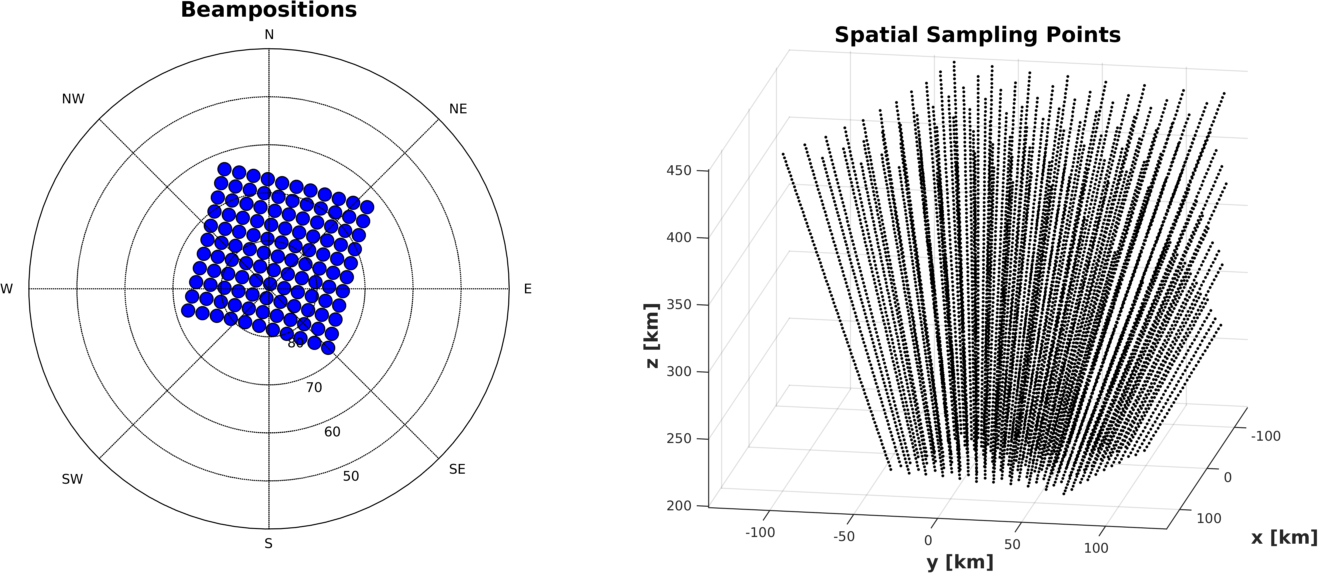
\includegraphics[width=6in]{Sampling3d}
\caption{The beam pattern used in angle space and the resulting 3-D spatial sampling pattern used for the three dimensional SimISR use case simulation.}
\label{fig:3dsampling}
\end{figure}

The input plasma parameters and the results of SimISR simulation are summarized in Figure \ref{fig:3dparams}.  For the selected configuration, the reconstructed density and ion temperature fields capture the predicted spatial variations reasonably well, providing confidence that this experimental configuration would result yield a positive detection of the spatial variations predicted by the applied FAC.  Reconstruction of the electron temperature enhancement (which is derived from a higher-order moment of the ISR spectrum) is less conclusive. This highlights the important point that variance is parameter dependent. In this case, SimISR informs us that, for this FAC and this experimental configuration, a negative result for $T_e$ comparison is not sufficient grounds to discount the model prediction.  A further refinement of the experiment might yield a positive result.

\begin{figure}[!h]
\centering
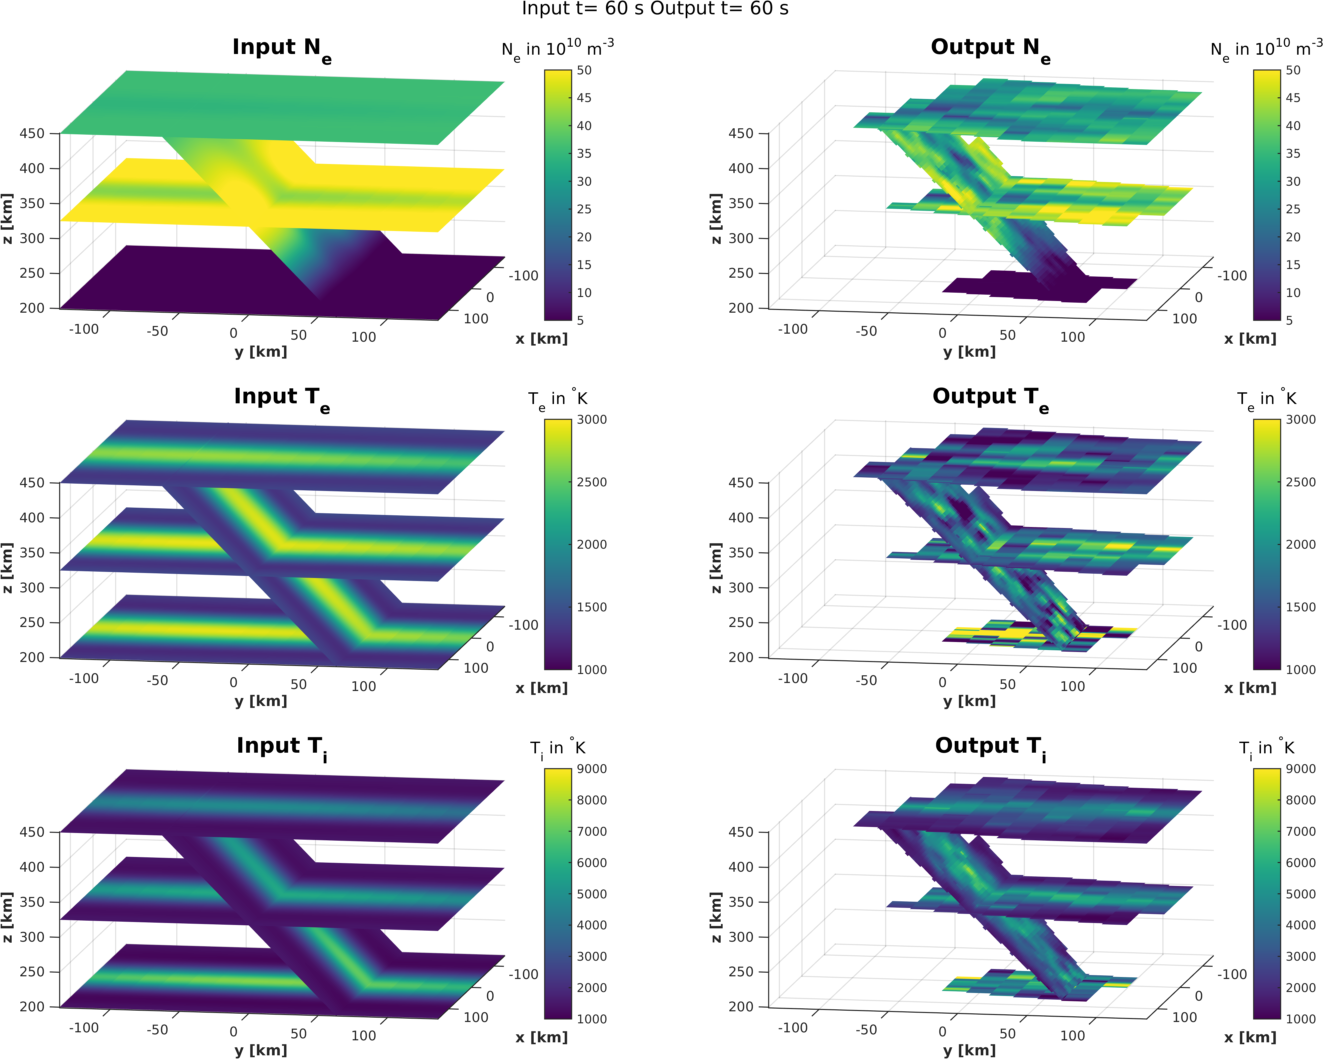
\includegraphics[width=6in]{60_60}
\caption{Input and output of full 3-D reconstruction of plasma parameters.}
\label{fig:3dparams}
\end{figure}

The sampling pattern picked for this simulation was chosen to get as dense a set of non-overlapping beams as possible.  This has been the general objective for several previous volumetric imaging experiments.
%% PJE: is this the main point? Or not?
%% JPS: This mode was designed off of a previous experiment although it is a very dense pattern.
The overall phenomena varies over a much larger area, so there is an obvious trade off between sampling density and the support region. These sorts of simulations can help experiment planners to understand these trade offs and possibly yield to innovative sampling stratagems for specific phenomena. 

\cleardoublepage

% -------------------------------------
% CHAPTER 6: CONCLUSION
% -------------------------------------
\chapter{Conclusions and Future Work}
\label{chapter:Conclusions}
\thispagestyle{myheadings}

% set this to the location of the figures for this chapter. it may
% also want to be ../Figures/2_Body/ or something. make sure that
% it has a trailing directory separator (i.e., '/')!
\graphicspath{{6_Conclusion/Figures/}}
This chapter contains conclusions, discussions and a summery of this dissertation. Part of the discussions will outline future work from the results of the thesis.

This thesis showed the outlined some of the basic theory behind ISR. It then followed with the modeling of the space-time ambiguity function which gives a forward model for ISR systems with electronically scanned arrays. A methodology to simulate complex voltage data for ISR was shown and is available as a software package called SimISR. Lastly using the space-time ambiguity a method to invert ISR data within the frame of reference of moving plasma and improve the resolution of the data has been developed. The inversion method was tested using SimISR in from a set of two-dimensional ionosphere plasma state parameters.

\section{Space-Time Ambiguity Function}
Section \ref{sec:sptimesamp} Section \ref{sec:sptimeamb} Section \ref{sec:frametrans} 
\section{SimISR}
Section \ref{sec:simex} Section \ref{sec:simmeth} Section \ref{sec:simex}
\section{Inversion of ISR Data}
Section \ref{sec:isrlit} Section \ref{sec:isralg} Section \ref{sec:results}
\section{Future Research Directions}

\subsection{Experiment Planning Using SimISR}

\subsection{Training Sets for Parameter Fits}

\subsection{Inversion Techniques}

\cleardoublepage

%\appendix
\begin{appendices}
\chapter{Ionosphere Incoherent Scatter Spectrum}
\label{appendix1}
\thispagestyle{myheadings}
\graphicspath{{Appendix/Figures/}}

%%%%%%%%%%%%%%%%%%%%%%%%%%%%%%%%%%%%%%%%%%%%%%%%%%%%%%%%%%%%%%%%%%%%%%%%%

This is the mathematical basis for calculating incoherent scatter spectrum for a given set of ionosphere state parameters. The appendix uses the methods developed \cite{kudeki:milla:1} and \cite{Kudeki:2006kx}.

\section*{Overall Formulation}
The first step comes from \cite{kudeki:milla:1} where a lumped circuit model is used to describe the spectrum. In it the independent thermal fluctuations of each species of ions and electrons are treated as current sources and the macroscopic conductances are treated as discrete components. The electric field $E$ impinged from the radar acts as a voltage. This lumped circuit model, seen in Figure \ref{fig:circuit}, is derived is taking the scalar component of Ampere's law in the direction of $\mathbf{k}$.  

\begin{equation}
\label{eq:ampere}
-j\mathbf{k} \times \mathbf{H} = \mathbf{J} +j\omega \epsilon_0 \mathbf{E},
\end{equation}

\noindent which then yields,

\begin{equation} 
\label{eq:ampscaler}
0=(\sigma_i +\sigma_e)E +\frac{\omega}{k}e(n_{ti}-n_{te}) +j\omega \epsilon_0 E.
\end{equation}

\begin{figure}[!h]
\centering
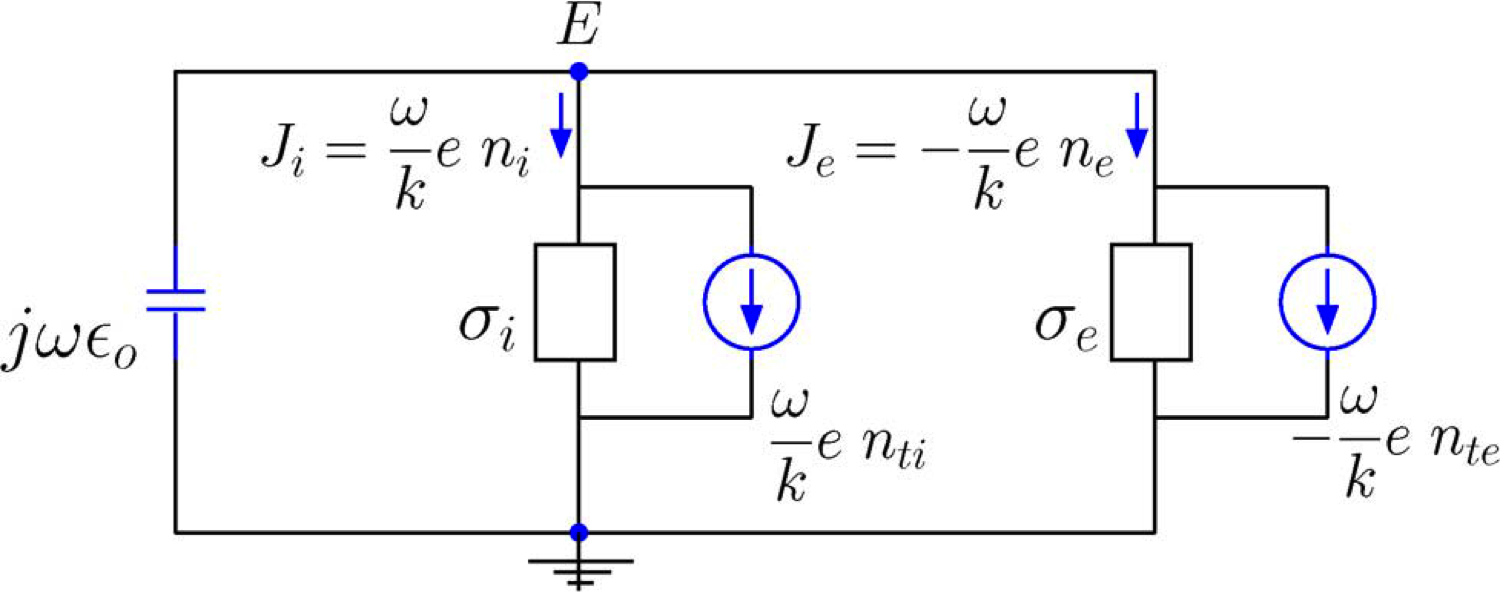
\includegraphics[width=3.0in]{circuit}
% where an .eps filename suffix will be assumed under latex, 
% and a .pdf suffix will be assumed for pdflatex; or what has been declared
% via \DeclareGraphicsExtensions.
\caption{Lumped circuit model seen in  \cite{kudeki:milla:1}.}
\label{fig:circuit}
\end{figure}

\noindent Using the electron current expression, $-\omega k^{-1}en_e = E\sigma_e -\omega k^{-1}en_{te}$, these equations can be rearranged to solve for $n_e$, 

\begin{equation}
\label{eq:neeq}
n_e(\mathbf{k},\omega) =  \frac{(j\omega\epsilon_0 + \sigma_i) n_{te}(\mathbf{k},\omega)}{j\omega\epsilon_0 +\sigma_e+\sigma_i} + \frac{\sigma_en_{ti}(\mathbf{k},\omega)}{j\omega\epsilon_0 +\sigma_e+\sigma_i}.
\end{equation}

\noindent To determine the power spectrum we square and average Equation \ref{eq:neeq} taking into account that the terms $n_{te}$ and $n_{ti}$ are independent of one and other we result in the following
\begin{equation}
\label{mainspeceq}
\langle \left|n_e(\mathbf{k},\omega)\right|^2\rangle = \frac{|j\omega\epsilon_0 + \sigma_i|^2 \langle |n_{te}(\mathbf{k},\omega)|^2\rangle}{|j\omega\epsilon_0 +\sigma_e+\sigma_i|^2} + \frac{| \sigma_e|^2 \langle |n_{ti}(\mathbf{k},\omega)|^2\rangle}{|j\omega\epsilon_0 +\sigma_e+\sigma_i|^2}.
\end{equation}

We can generalize them for multiple ion species by simply summing over the thermal fluctuations and conductances in Equation \ref{eq:ampscaler},

\begin{equation} 
\label{eq:ampscalersum}
0=\left(\displaystyle \sum_k^K\sigma_{ik} +\sigma_e\right)E +\frac{\omega}{k}e\left(\sum_k^Kn_{tik}-n_{te}\right) +j\omega \epsilon_0 E.
\end{equation}

\noindent This then augments the power spectrum in Equation \ref{mainspeceq} to the following

\begin{equation}
\label{eq:sumspeceq}
\displaystyle \langle \left|n_e(\mathbf{k},\omega)\right|^2\rangle = \frac{\left|j\omega\epsilon_0 +  \sum_k^K\sigma_{ik} \right|^2 \langle |n_{te}(\mathbf{k},\omega)|^2\rangle}{\left|j\omega\epsilon_0 +\sigma_e+ \sum_k^K\sigma_{ik} \right|^2} + \frac{| \sigma_e|^2 \left \langle \left|\sum_k^Kn_{tik}(\mathbf{k},\omega)\right|^2\right\rangle}{\left|j\omega\epsilon_0 +\sigma_e+ \sum_k^K\sigma_{ik} \right|^2}.
\end{equation}

%%%%%%%%%%%%%%%%%%%%%%%%%%%%%%%%%%%%%%%%%%%%%%%%%%%%%%%%%%%%%%%%%%%%%%
\section*{Gordeyeve Integrals}
The power spectrum of the thermal fluctuation for each species $s$ can be determined by the following,

\begin{equation}
\label{eq:thermalfl}
\frac{\langle|n_{ts}(\mathbf{k},\omega)|^2\rangle}{N_s} = 2\text{Re}\{J_s(\omega_s)\},
\end{equation}

\noindent where $N_s$ is the average density for the species.  Also the conductance for each species $s$ can be determine from the following,

\begin{equation}
\label{eq:cond}
\frac{\sigma_{s}(\mathbf{k},\omega)}{j\omega\epsilon_0} = \frac{1-j\omega_s J_s(\omega_s)}{k^2\lambda_s^2}
\end{equation}

\noindent where $\omega_s \equiv \omega-\mathbf{k}\cdot\mathbf{V}_s $ is the Doppler shifted frequency and $\lambda_s \equiv \sqrt{\frac{\epsilon_0 KT_s}{N_s q_s^2}}$ is the Debye length for each species.

The $J_s$ terms can be represented as follows

\begin{equation}
\label{eq:gord}
J_s(\omega)\equiv \int_0^\infty \langle e^{j\mathbf{k}\cdot\Delta \mathbf{r}_s}\rangle e^{j\omega\tau}d\tau
\end{equation}

\noindent These terms are known as Gordeyeve integrals, which are the one sided Fourier transforms of the characteristic functions of the particle displacements $\langle e^{j\mathbf{k}\cdot\Delta\mathbf{r}_s}\rangle$.  

The particle displacement function can change depending on magnetic field and collisionality of the plasma. For the high latitude F-region in the ionosphere a case of general importance is one of a non-magnitized and collision less plasma, where $\Delta\mathbf{r} = \mathbf{v}\tau$ where $\tau$ is the time interval. Assuming a Maxwellian the PDF of one dimensional displacement is

\begin{equation}
\label{eq:pdfr}
f(\Delta r) = \frac{1}{\sqrt{2\pi \langle r^2 \rangle}}e^{\frac{-\Delta r^2}{2\langle r^2\rangle}}.
\end{equation}
 
\noindent The variance term $\langle r^2 \rangle$ can be represented as
\begin{equation}
\label{eq:var}
\langle r^2 \rangle = \langle v^2 \rangle \tau^2 = \frac{KT_s}{m_s} \tau^2
\end{equation}
 \noindent where $T_s$ is the temperature of the species, $K$ is Boltzmans constant and $m_s$ is the mass of the species in kg. To simplify notation like in \cite{kudeki:milla:1}, we will refer to $\sqrt{KT_s/m_s}$ as $C$. Which yields the following single particle ACF,
 
 \begin{equation}
\label{eq:pdfall}
\langle e^{j\mathbf{k}\cdot\Delta \mathbf{r}}\rangle= e^{-\frac{1}{2}k^2C^2 \tau^2}.
\end{equation}
 
 To model collisions we use the term $\nu$ as the collision frequency for the species. If $\nu<<kC$ then \ref{eq:pdfall} can be used as the single particle ACF. If not the following must be used.
 
 \begin{equation}
 \label{eq:colspacf}
 \langle e^{j\mathbf{k}\cdot\Delta \mathbf{r}}\rangle = e^{-\frac{k^2C^2}{\nu^2}\left( \nu \tau-1+e^{-\nu\tau}\right)}
 \end{equation}
 
Lastly if one is to add a magnetic field to the equations the single particle ACFs must now take into a account the orientation of the magnetic field. The authors of \cite{kudeki:milla:1} use the convention of breaking up the Bragg vector $\mathbf{k}$ into two components, one parallel to the magnetic field, $k_{\parallel}$ and one perpendicular,$k_{\perp}$, as such, $\mathbf{k}= \hat{b}k_{\parallel}+\hat{p}k_{\perp}$. This yields the following formulation for the single particle ACF,

 \begin{equation}
\label{eq:pdfmag}
\langle e^{j\mathbf{k}\cdot\Delta \mathbf{r}}\rangle= e^{-\frac{1}{2}k_{\parallel}^2C^2 \tau^2}\times e^{-\frac{2k_{\perp}^2C^2}{\Omega^2} \sin^2(\Omega\tau/2)},
\end{equation}

\noindent where the gyro frequency is $\Omega = qB/m$This formulation neglects the effects of collisions which if taken into account yields the following single particle ACF,

\begin{equation}
\label{eq:colspacf}
\langle e^{j\mathbf{k}\cdot\Delta \mathbf{r}}\rangle = e^{-\frac{k_\parallel^2C^2}{\nu^2}\left( \nu \tau-1+e^{-\nu\tau}\right)}\times e^{-\frac{k_\perp^2C^2}{\nu^2+\Omega^2}\left(\cos(2\gamma) + \nu \tau-e^{-\nu\tau}\cos(\Omega\tau-2\gamma)\right)},
\end{equation}
 
\noindent where $\gamma = \tan^{-1}(\nu\Omega)$. The for the case with the magnetic field as one gets closer to being fulling perpendicular to $\mathbf{B}$ the single particle ACFs become much more narrow band, to the point of becoming delta functions in the frequency space. It is necessary to use other methods beyond numerical integration to determine the Gordeyeve Integrals. The authors of \cite{kudeki:milla:2} get around this problem by making a particle in cell simulation to determine the particle statistics. 


%%%%%%%%%%%%%%%%%%%%%%%%%%%%%%%%%%%%%%%%%%%%%%%%%%%%%%%%%%%%%%%%%%%%%%
 \section*{Computational Considerations}
One of the main challenges to calculating the ISR spectrums is calculating the Gordeyeve integrals. The case with no collisions or magnetic fields can be done analytically using Dawsons integral. This can be done using the identity

\begin{equation}
\label{eq:daw1}
jZ(\theta) = \int_0^{\infty} e^{-j\theta t}e^{-\frac{t^2}{4}}dt = \sqrt{\pi}e^{-\theta^2}-j2e^{-\theta^2}\int_0^\theta e^{t^2}dt.
\end{equation}

\noindent Using the terms found in Equation \ref{eq:pdfall}, $\theta=\omega_s/\left(\sqrt{2}kC\right)$ and $t=\sqrt{2}kC\tau$.

For other cases where analytical calculation is not possible a numerical integration scheme from \cite{Ooi:2007jx} is used. It is also possible to use a Chirp-z based algorithm that is shown in \cite{Li:1991gr} from the experiences of the author the first technique converges faster. The technique used in \cite{Ooi:2007jx} changes the variable of integration for integrals of the following form,

\begin{equation}
\label{eq:Sommer}
I=\int_a^b f(z) dz.
\end{equation}

\noindent The technique changes the variable $z$ in the following way,

\begin{equation}
\label{eq:newz}
z = \frac{1}{2}(a+b)+\frac{1}{2} (b-a)\text{Erf}(g(t)),
\end{equation}

\noindent where $g(t)$ is a function that is choosen so  $g(t)\rightarrow\pm \infty$ as $t\rightarrow\pm \infty$ and $Erf(u)$ is 
\begin{equation}
\label{eq:erf1}
\text{Erf}(u) = \frac{2}{\sqrt{\pi}}\int_0^u e^{-t^2}dt.
\end{equation}

\noindent Discretizing and changing variables the integral in Equation \ref{eq:Sommer} becomes the following sum

\begin{equation}
\label{eq:erfsum1}
I=\displaystyle \sum_{n=-N}^N A_nf\left( \frac{1}{2}(a+b)+\frac{1}{2} (b-a)\text{Erf}(g(nh))\right)
\end{equation}

\noindent where,
\begin{equation}
\label{eq:anterm}
A_n = g'(nh)e^{-g(nh)^2}.
\end{equation}

\noindent Like in \cite{Ooi:2007jx}, $g(nh) = \sinh (nh)$ and the grid spacing $h$ is the following,

\begin{equation}
\label{eq:hterm}
h = \frac{1}{N}\ln(1.05\sqrt{2}N).
\end{equation} 


Lastly to avoid cases of divid by zero errors the main equations have to be rearrange slightly. First off because some ion species could have zero density Equation \ref{eq:cond} uses the Debye length of the electron species,$\lambda_e$ as follows

\begin{equation}
\label{eq:condnew}
\frac{\sigma_{s}(\mathbf{k},\omega)}{j\omega\epsilon_0} = \frac{1-j\omega_s J_s(\omega_s)}{k^2\lambda_e^2} \left(\frac{q_sT_eN_s}{q_eT_sN_e}\right).
\end{equation}

Also, to avoid having to more calculations then necessary the $j\omega\epsilon_0$. terms of Equation \ref{eq:sumspeceq} are moved around. Thus it becomes,

\begin{equation}
\label{eq:sumspeceqfinal}
\displaystyle \langle \left|n_e(\mathbf{k},\omega)\right|^2\rangle =  \frac{\left|1 +  \sum_k^K\frac{\sigma_{ik}}{j\omega\epsilon_0} \right|^2 \langle |n_{te}(\mathbf{k},\omega)|^2\rangle}{\left|1 +\frac{\sigma_e+ \sum_k^K\sigma_{ik}}{j\omega\epsilon_0} \right|^2} + \frac{\left| \frac{\sigma_e}{j\omega\epsilon_0} \right|^2\left \langle \left|\sum_k^Kn_{tik}(\mathbf{k},\omega)\right|^2\right\rangle}{\left|1 +\frac{\sigma_e+ \sum_k^K\sigma_{ik}}{j\omega\epsilon_0} \right|^2}.
\end{equation}

\noindent If the Gordeyeve integrals are substitute in Equation \ref{eq:sumspeceqfinal} it becomes the following.

\begin{equation}
\label{eq:sumspeceqactual}
\begin{split}
\displaystyle \langle \left|n_e(\mathbf{k},\omega)\right|^2\rangle =&  \frac{\left|1 + \sum_s^K  \frac{1-j\omega_s J_s(\omega_s)}{k^2\lambda_e^2} \left(\frac{q_sT_eN_s}{q_eT_sN_e}\right) \right|^2 2N_e\text{Re}\{J_e(\omega_e)\}}{\left|1 + \frac{1-j\omega_e J_e(\omega_e)}{k^2\lambda_e^2}  +\sum_s^K  \frac{1-j\omega_s J_s(\omega_s)}{k^2\lambda_e^2} \left(\frac{q_sT_eN_s}{q_eT_sN_e}\right) \right|^2}       + \\        & \frac{\left| \frac{1-j\omega_s J_e(\omega_e)}{k^2\lambda_e^2} \right|^2\sum_s^K  2N_s\text{Re}\{J_s(\omega_s)\}}{\left|1 + \frac{1-j\omega_e J_e(\omega_e)}{k^2\lambda_e^2}  +\sum_s^K  \frac{1-j\omega_s J_s(\omega_s)}{k^2\lambda_e^2} \left(\frac{q_sT_eN_s}{q_eT_sN_e}\right) \right|^2}.
\end{split}
\end{equation}

\section*{Examples}
We can see in Figure \ref{fig:diffspectrums} examples of ISR spectrums from different ISR systems. The spectrums were generated using the the parameters values $N_e=1\times10^{11}$, $T_e=3000^o$K and $T_i=3000^o$K and the system parameter values seen in Table \ref{tab:ISRsys}. The ion acoustic frequency$f_{ia}$ for each system with the following plasma parameters its wavelength $\lambda$ was calculated using the following formula,

\begin{equation}
\label{eq:iaf}
f_{ia} = \frac{\lambda}{2}\sqrt{\frac{k_bT_e +k_b\gamma_iT_i}{M}},
\end{equation}

\noindent where $M$ is the ion mass in kg, $k_b$ is Botlzmann's constant and $\gamma_i$ is the adiabatic index which is set to 3 in all cases. In most of the cases the familiar double hump spectrum is visible. The only exception to this is Jicamarca, where the system's k-vector is very close to being perpendicular to the earths magnetic field. This also impacts the amount of time it takes to calculate the spectrum because as the k-vector gets closer to being perpendicular to magnetic field the Gordeyeve integral will take longer to converge.
\begin{figure}[!h]
\centering
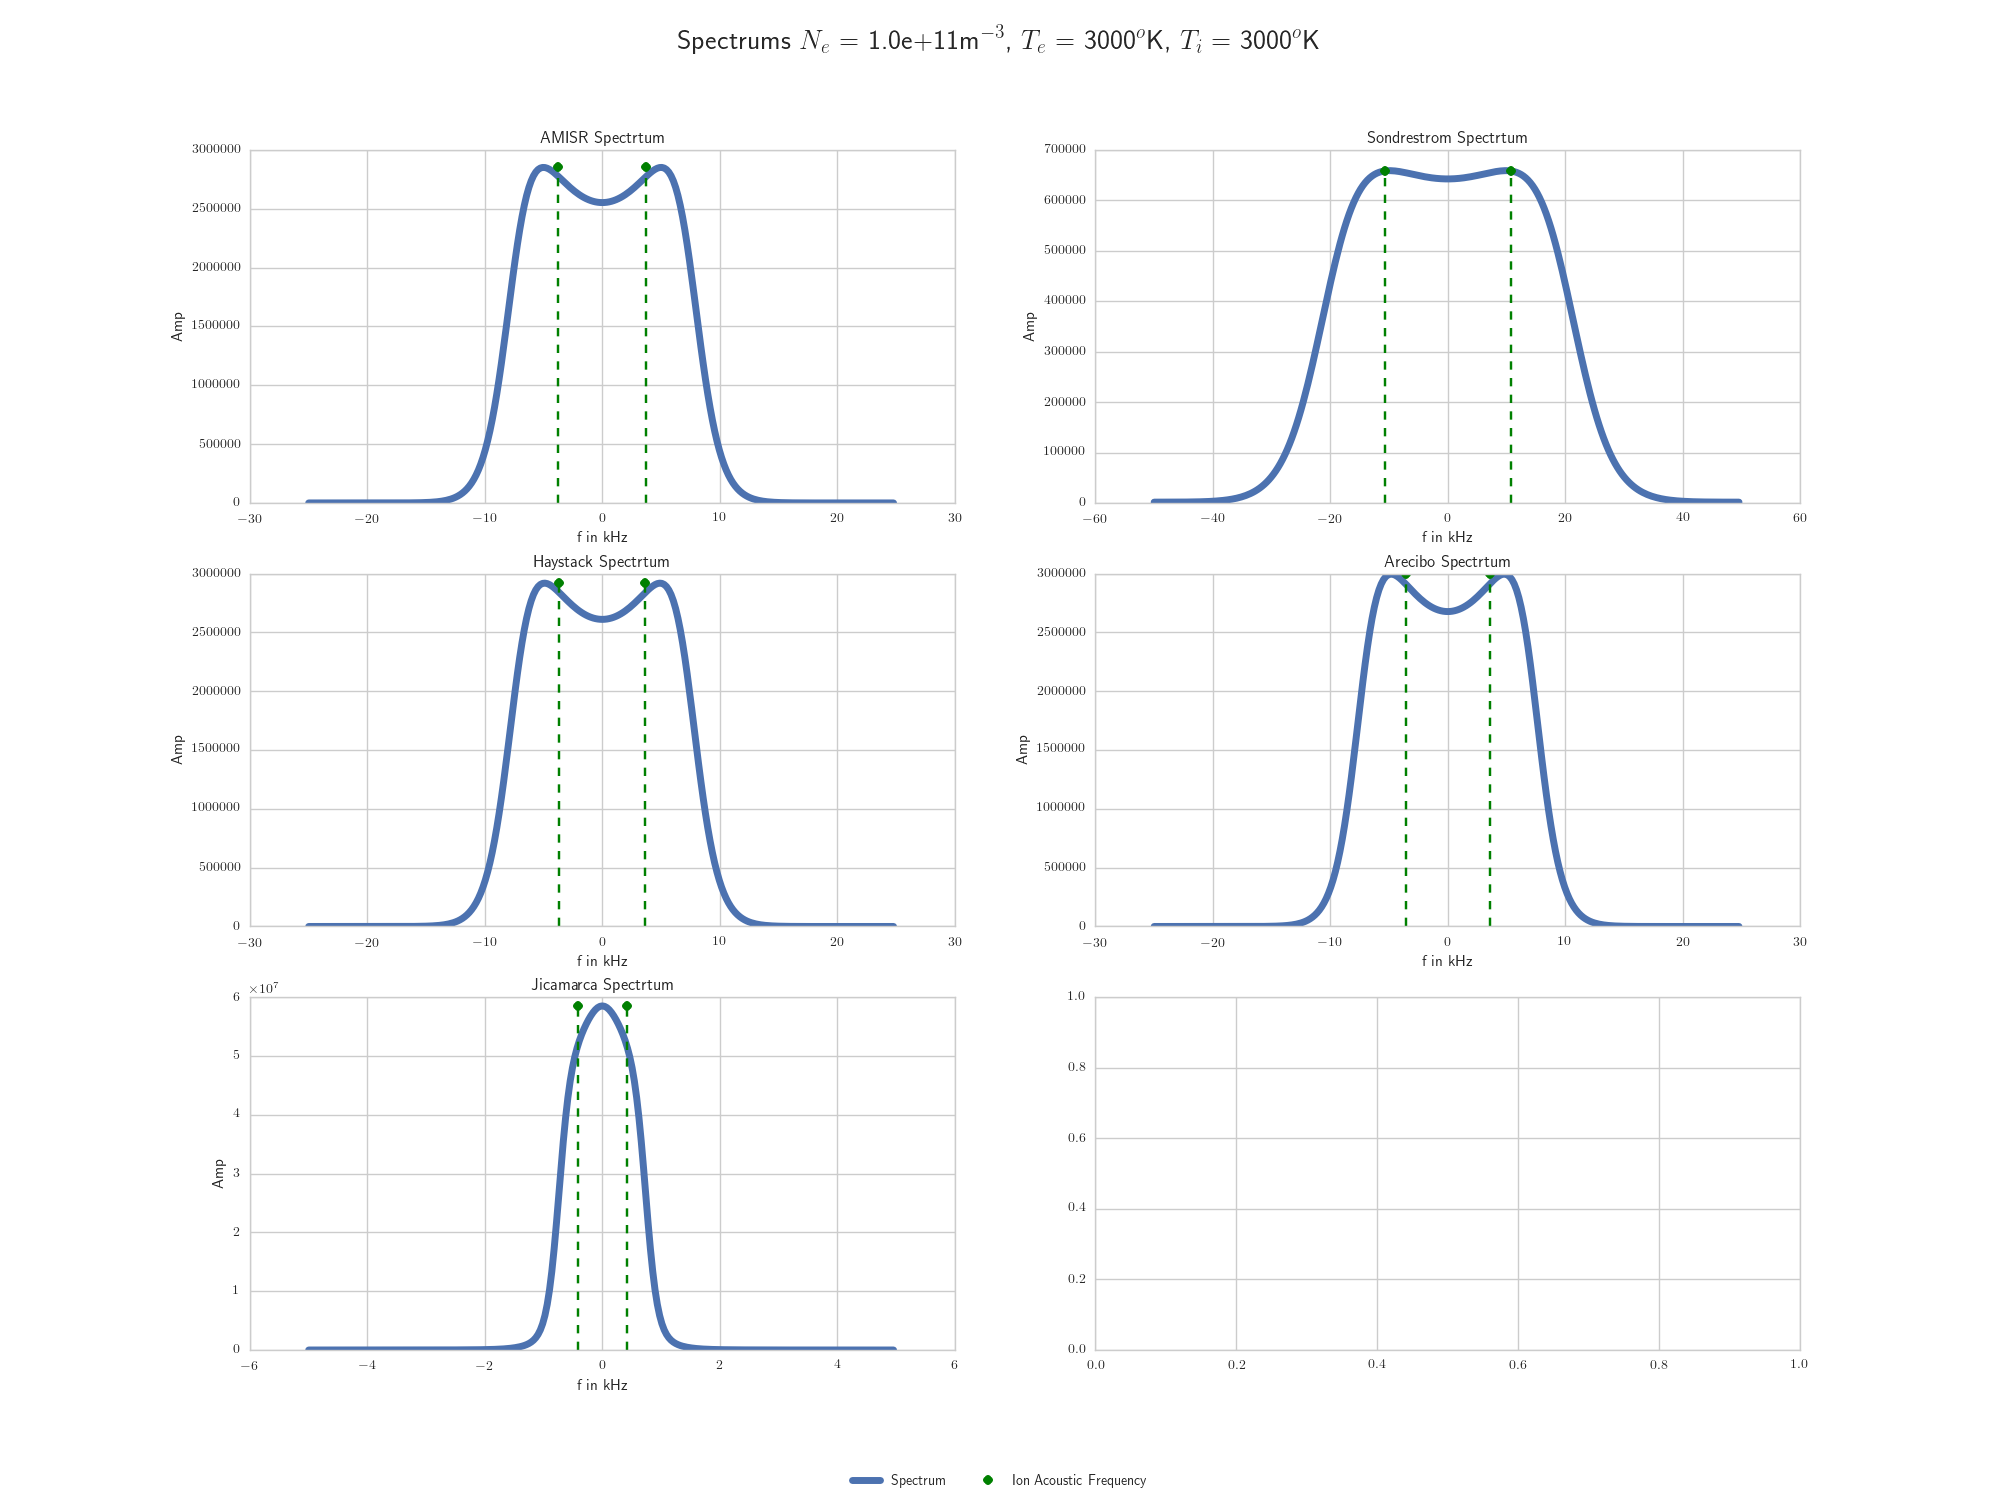
\includegraphics[width=7.0in]{DifferentSystems}

\caption{Spectrums From Different ISR Systems}
\label{fig:diffspectrums}
\end{figure}


\begin{table}[!h]
\centering
\caption{ISR System Parameters}
\label{tab:ISRsys}
\begin{tabular}{lllll}
System Name & $f_0$ in MHz & $f_s$ in kHz & $\alpha$ in $^o$ &  \\
AMISR       & 449          & 50           & 70               &  \\
Sondrestrom & 1290         & 100          & 80               &  \\
Haystack    & 440          & 50           & 65               &  \\
Arecibo     & 430          & 50           & 45               &  \\
Jicamarca   & 50           & 10           & 1                & 
\end{tabular}
\end{table}
\end{appendices}
%==========================================================================%
% Bibliography
\newpage
\singlespace
\bibliographystyle{apalike}

% each subdirectory can have its own BiBTeX file
\bibliography{BibTex/litreview.bib}
\cleardoublepage

%==========================================================================%
% Curriculum Vitae
\addcontentsline{toc}{chapter}{Curriculum Vitae}

\thispagestyle{empty}

\begin{center}
{\LARGE {\bf CURRICULUM VITAE}}\\
\vspace{0.5in}
{\large {\bf John Swoboda}}
\end{center}

\section*{EDUCATION}{\sl PhD,} Electrical Engineering, Fall 2016; Expected \\
                      % \sl will be bold italic in New Century Schoolbook (or
	              % any postscript font) and just slanted in
		      %	Computer Modern (default) font
                GPA 3.90/4.00 \\
                Boston University, Boston, MA
	       

{\sl Master of Science,} Electrical Engineering, May 2008 \\
                      % \sl will be bold italic in New Century Schoolbook (or
	              % any postscript font) and just slanted in
		      %	Computer Modern (default) font
                 GPA 3.71/4.00\\
                Thesis Title: Reconstruction of Tomographic Images Corrupted by a Slice Sensitivity Profile With Applications to The Inspection of Manufactured Items\\
 {\sl Bachelor of Science,} Electrical \& Computer Systems Engineering, May 2007  \\
                GPA: 3.74/4.00\\
                Rensselaer Polytechnic Institute, Troy, NY, \\
                
 
 

 
\section*{RELEVENT \\ EXPERIENCE}
 {\sl Research Assistant} \hfill            September 2012 - Present \\
                Electrical Engineering Department, Boston University 
                 \begin{itemize}  \itemsep -2pt %reduce space between items
                 \item Performed data fusion and analysis from varied sensor types for geophysical research.
                 \item Created theoretical frame work for incoherent scatter radar data processing.
                 \item Developed simulations, algorithms for incoherent scatter radar systems.
                 \end{itemize} 

 {\sl Sensor System Engineer} \hfill January 2009 - August 2012\\
                The MITRE Corporation, Bedford MA 
                 	\begin{itemize}  \itemsep -2pt %reduce space between items
                	\item Developed new algorithms for experimental radar systems.
                	\item Created full signal processing level emulations and simulations of radar systems.
                \end{itemize}
 
                {\sl Research Assistant} \hfill            May 2009 - January 2009 \\
                Electrical Engineering Department, Rensselaer Polytechnic Institute 
                 \begin{itemize}  \itemsep -2pt %reduce space between items
                 \item Developed signal processing algorithms applied to image formation radar.
                 \end{itemize} 
                {\sl Research Engineering Intern} \hfill        May 2007 - May 2008\\
                Lickenbrock Technologies, Troy NY
                  \begin{itemize}
                   \item Developed signal processing algorithms for the deblurring of tomographic images.
                   \end{itemize} 
\section*{COMPUTER \\ SKILLS} {\sl Languages \& Software:} Python, MATLAB, C, C$++$, \LaTeX, Git, Microsoft Office.\\
                {\sl Operating Systems:} Mac OS X, Linux, Windows. 
 
\section*{PUBLICATIONS}   

\begin{itemize}
	\item Swoboda, J., Semeter J., Improvement of Resolution of Incoherent Scatter Radar Using Electronically Scanned Arrays and Inverse Theory, IEEE Symposium on Phased Array Technology, 2016
	\item Swoboda, J., Semeter J., Erickson, P., Zettergren M., Observability of Ionospheric Space-Time Structure with ISR:   A Simulation Study, (To be Submitted). 
	\item Swoboda, J., J. Semeter, and P. Erickson (2015), Space-time ambiguity functions for electronically scanned ISR applications, Radio Sci., 50, 2015. DOI: 10.1002/2014RS005620

	\item Krishnan, V., Swoboda, J., Yarman, C.E., Yazici, B. , Multistatic Synthetic Aperture Radar Image Formation, IEEE Transactions on Image Processing , vol.19, no.5, pp.1290-1306, May 2010
    \item  Swoboda, J., Yarman, C. E., Yazici, B., Bistatic synthetic aperture radar imaging for arbitrary trajectories in the presence of noise and clutter. Proc. SPIE 7307, Airborne Intelligence, Surveillance, Reconnaissance (ISR) Systems and Applications VI, 73070D April 28, 2009 
\end{itemize}
	
\section*{PRESENTATIONS}
\begin{itemize}
	\item Swoboda, J., Hirsch, M.,Semeter, J., GeoData Python Toolset: High Performance Python for Geoscience, CEDAR Workshop, 2016
    \item Swoboda, J.,  Semeter, J., The "Impulse Response" of Electronically Scanned and Dish Based ISR, URSI, 2016
    \item Swoboda, J., Semeter J., Erickson, P., Zettergren M., Impact of the Forward Model of ESA Based ISR on Measurements from HAARP, CEDAR, 2015
	\item Swoboda, J., Semeter J., Erickson, P., Zettergren M., Three Dimensional Ionosphere Reconstruction from Electronically Steerable ISR, MTSSP, 2015
	\item Swoboda, J., Dahlgren, H., Semeter J., Erickson, P., On the Way to Optimal Processing for Multi-beam RISR Experiments, CEDAR, 2014
    \item Swoboda, J., Semeter J., Erickson, P., Simulation of ISR Data and Application to Spatial Sampling of the Ionosphere, URSI, 2015
\end{itemize}

\section*{POSTER \\ PRESENTATIONS}
\begin{itemize}
\item Swoboda, J., Semeter J., Improvement of Resolution of Incoherent Scatter Radar Using Electronically Scanned Arrays and Inverse Theory, NEROC Symposium, 2016
\item Swoboda, J., Semeter J., Improvement of Resolution of Incoherent Scatter Radar Using Electronically Scanned Arrays and Inverse Theory, IEEE Symposium on Phased Array Technology, 2016
\item Swoboda, J.,  Semeter, J., Resolving Cross Range Gradients in the High Latitude Ionosphere, CEDAR Workshop, 2016
\item Swoboda, J., Hirsch, M.,Semeter, J., GeoData: A Generalized Data Analysis Software Suite, CEDAR Workshop, 2015
\item Swoboda, J., Dahlgren, H., Semeter J., Erickson, P., Plasma Motion Induced Artifacts in 3-D Incoherent Scatter Radar, CEDAR, 2014
\end{itemize}

\section*{CODE / DATASETS}
\begin{itemize}
\item J. Swoboda, M. Hirsch, A. Stuhlmacher, G. Starr, and Semeter, J. (2016). GeoData Python [code]. Zenodo. http://doi.org/10.5281/zenodo.154533
\end{itemize}
 

%==========================================================================%
\end{document}
